% Options for packages loaded elsewhere
\PassOptionsToPackage{unicode}{hyperref}
\PassOptionsToPackage{hyphens}{url}
\PassOptionsToPackage{dvipsnames,svgnames,x11names}{xcolor}
%
\documentclass[
  11pt,
  letterpaper,
]{scrreprt}

\usepackage{amsmath,amssymb}
\usepackage{iftex}
\ifPDFTeX
  \usepackage[T1]{fontenc}
  \usepackage[utf8]{inputenc}
  \usepackage{textcomp} % provide euro and other symbols
\else % if luatex or xetex
  \usepackage{unicode-math}
  \defaultfontfeatures{Scale=MatchLowercase}
  \defaultfontfeatures[\rmfamily]{Ligatures=TeX,Scale=1}
\fi
\usepackage{lmodern}
\ifPDFTeX\else  
    % xetex/luatex font selection
  \setmainfont[]{TeX Gyre Pagella}
\fi
% Use upquote if available, for straight quotes in verbatim environments
\IfFileExists{upquote.sty}{\usepackage{upquote}}{}
\IfFileExists{microtype.sty}{% use microtype if available
  \usepackage[]{microtype}
  \UseMicrotypeSet[protrusion]{basicmath} % disable protrusion for tt fonts
}{}
\makeatletter
\@ifundefined{KOMAClassName}{% if non-KOMA class
  \IfFileExists{parskip.sty}{%
    \usepackage{parskip}
  }{% else
    \setlength{\parindent}{0pt}
    \setlength{\parskip}{6pt plus 2pt minus 1pt}}
}{% if KOMA class
  \KOMAoptions{parskip=half}}
\makeatother
\usepackage{xcolor}
\setlength{\emergencystretch}{3em} % prevent overfull lines
\setcounter{secnumdepth}{5}
% Make \paragraph and \subparagraph free-standing
\ifx\paragraph\undefined\else
  \let\oldparagraph\paragraph
  \renewcommand{\paragraph}[1]{\oldparagraph{#1}\mbox{}}
\fi
\ifx\subparagraph\undefined\else
  \let\oldsubparagraph\subparagraph
  \renewcommand{\subparagraph}[1]{\oldsubparagraph{#1}\mbox{}}
\fi


\providecommand{\tightlist}{%
  \setlength{\itemsep}{0pt}\setlength{\parskip}{0pt}}\usepackage{longtable,booktabs,array}
\usepackage{calc} % for calculating minipage widths
% Correct order of tables after \paragraph or \subparagraph
\usepackage{etoolbox}
\makeatletter
\patchcmd\longtable{\par}{\if@noskipsec\mbox{}\fi\par}{}{}
\makeatother
% Allow footnotes in longtable head/foot
\IfFileExists{footnotehyper.sty}{\usepackage{footnotehyper}}{\usepackage{footnote}}
\makesavenoteenv{longtable}
\usepackage{graphicx}
\makeatletter
\def\maxwidth{\ifdim\Gin@nat@width>\linewidth\linewidth\else\Gin@nat@width\fi}
\def\maxheight{\ifdim\Gin@nat@height>\textheight\textheight\else\Gin@nat@height\fi}
\makeatother
% Scale images if necessary, so that they will not overflow the page
% margins by default, and it is still possible to overwrite the defaults
% using explicit options in \includegraphics[width, height, ...]{}
\setkeys{Gin}{width=\maxwidth,height=\maxheight,keepaspectratio}
% Set default figure placement to htbp
\makeatletter
\def\fps@figure{htbp}
\makeatother
% definitions for citeproc citations
\NewDocumentCommand\citeproctext{}{}
\NewDocumentCommand\citeproc{mm}{%
  \begingroup\def\citeproctext{#2}\cite{#1}\endgroup}
\makeatletter
 % allow citations to break across lines
 \let\@cite@ofmt\@firstofone
 % avoid brackets around text for \cite:
 \def\@biblabel#1{}
 \def\@cite#1#2{{#1\if@tempswa , #2\fi}}
\makeatother
\newlength{\cslhangindent}
\setlength{\cslhangindent}{1.5em}
\newlength{\csllabelwidth}
\setlength{\csllabelwidth}{3em}
\newenvironment{CSLReferences}[2] % #1 hanging-indent, #2 entry-spacing
 {\begin{list}{}{%
  \setlength{\itemindent}{0pt}
  \setlength{\leftmargin}{0pt}
  \setlength{\parsep}{0pt}
  % turn on hanging indent if param 1 is 1
  \ifodd #1
   \setlength{\leftmargin}{\cslhangindent}
   \setlength{\itemindent}{-1\cslhangindent}
  \fi
  % set entry spacing
  \setlength{\itemsep}{#2\baselineskip}}}
 {\end{list}}
\usepackage{calc}
\newcommand{\CSLBlock}[1]{\hfill\break\parbox[t]{\linewidth}{\strut\ignorespaces#1\strut}}
\newcommand{\CSLLeftMargin}[1]{\parbox[t]{\csllabelwidth}{\strut#1\strut}}
\newcommand{\CSLRightInline}[1]{\parbox[t]{\linewidth - \csllabelwidth}{\strut#1\strut}}
\newcommand{\CSLIndent}[1]{\hspace{\cslhangindent}#1}


% Wird für die Tabelle im Titelblatt der Experten verwendet:
% Array
\usepackage{array}
% Neue Definition für Tabelleneinträge
% linksbündig mit Breitenangabe
\newcolumntype{L}[1]{>{\raggedright\arraybackslash}p{#1}} 
% zentriert mit Breitenangabe
\newcolumntype{C}[1]{>{\centering\arraybackslash}p{#1}} 
% rechtsbündig mit Breitenangabe
\newcolumntype{R}[1]{>{\raggedleft\arraybackslash}p{#1}} 

\usepackage[a4paper, margin=3cm]{geometry}

% Titles take mainfont
\addtokomafont{disposition}{\rmfamily}





\makeatletter
\@ifpackageloaded{bookmark}{}{\usepackage{bookmark}}
\makeatother
\makeatletter
\@ifpackageloaded{caption}{}{\usepackage{caption}}
\AtBeginDocument{%
\ifdefined\contentsname
  \renewcommand*\contentsname{Inhaltsverzeichnis}
\else
  \newcommand\contentsname{Inhaltsverzeichnis}
\fi
\ifdefined\listfigurename
  \renewcommand*\listfigurename{Abbildungsverzeichnis}
\else
  \newcommand\listfigurename{Abbildungsverzeichnis}
\fi
\ifdefined\listtablename
  \renewcommand*\listtablename{Tabellenverzeichnis}
\else
  \newcommand\listtablename{Tabellenverzeichnis}
\fi
\ifdefined\figurename
  \renewcommand*\figurename{Abbildung}
\else
  \newcommand\figurename{Abbildung}
\fi
\ifdefined\tablename
  \renewcommand*\tablename{Tabelle}
\else
  \newcommand\tablename{Tabelle}
\fi
}
\@ifpackageloaded{float}{}{\usepackage{float}}
\floatstyle{ruled}
\@ifundefined{c@chapter}{\newfloat{codelisting}{h}{lop}}{\newfloat{codelisting}{h}{lop}[chapter]}
\floatname{codelisting}{Listing}
\newcommand*\listoflistings{\listof{codelisting}{Listingverzeichnis}}
\makeatother
\makeatletter
\makeatother
\makeatletter
\@ifpackageloaded{caption}{}{\usepackage{caption}}
\@ifpackageloaded{subcaption}{}{\usepackage{subcaption}}
\makeatother
\ifLuaTeX
\usepackage[bidi=basic]{babel}
\else
\usepackage[bidi=default]{babel}
\fi
\babelprovide[main,import]{ngerman}
\ifPDFTeX
\else
\babelfont{rm}[]{TeX Gyre Pagella}
\fi
% get rid of language-specific shorthands (see #6817):
\let\LanguageShortHands\languageshorthands
\def\languageshorthands#1{}
\ifLuaTeX
  \usepackage{selnolig}  % disable illegal ligatures
\fi
\usepackage{bookmark}

\IfFileExists{xurl.sty}{\usepackage{xurl}}{} % add URL line breaks if available
\urlstyle{same} % disable monospaced font for URLs
\hypersetup{
  pdftitle={Tragverhalten von Stahlbetontragwerken},
  pdfauthor={Pascal Gitz},
  pdflang={de},
  colorlinks=true,
  linkcolor={Black},
  filecolor={Maroon},
  citecolor={Blue},
  urlcolor={Blue},
  pdfcreator={LaTeX via pandoc}}

% TITELBLATT, VERSIONSTABELLE UND SELBSTSTÄNDIGKEITSERKLÄRUNG
%--------------------------------------------------------------------------------------------------------------------


\titlehead{\includegraphics[height=0.5cm]{../imgs/logos/logo-mse}\hfill\includegraphics[height=0.5cm]{../imgs/logos/logo-hslu-en-col} \\ }
\subject{MASTER OF SCIENCE IN ENGINEERING\\Vertiefungsmodul II}
\title{Tragverhalten von Stahlbetontragwerken}

\subtitle
{Modellvorstellungen zur nichtlinearen Verformungsberechnung}

%\thanks{
%Version 1.0
%\hfill \today
%\hfill Hun}


\date{\large Horw, Freitag, 14. Juni 2024}
\author{Pascal Gitz}

\publishers{
	\begin{table}[H]
		\centering
		\begin{tabular}{L{2cm} L{6cm}}
			Advisor: & Prof. FH, Dr. Daniel Heinzmann \\
			Experte: & Dr. Thomas Jäger \\
		\end{tabular}
	\end{table}
}
\begin{document}
\maketitle


Hiermit erkläre ich, dass ich die vorliegende Arbeit selbstständig angefertigt und keine anderen als die angegebenen Hilfsmittel verwendet habe. Sämtliche verwendeten Textausschnitte, Zitate oder Inhalte anderer Verfasser wurden ausdrücklich als solche gekennzeichnet.\\%
%
\\%
%
Horw, 14. Juni 2024 \hfill Pascal Gitz%

\vfill
%\begin{tabular}[h]{llcr} 
    %*Version 2.0 & - Definitives Exemplar & \today & MK \\ 
    %*Version 1.0 & - Prüfungsexemplar & 22. Januar 2021 & MK \\ 
%\end{tabular}\\

% Version 2.0 - Definitives Exemplar \hfill \today \quad \quad \quad \quad \quad MK\\
Version 1.0 - Prüfungsexemplar \hfill 14. Juni 2024 \quad \quad \quad \quad \quad PG\\
Version 0.9 - Entwurf \hfill 07. Juni 2024 \quad \quad \quad \quad \quad PG\\

\newpage

\chapter*{Kurzfassung}

Diese Arbeit ist Teil einer Arbeitsserie, bestehend aus dem Vertiefungsmodul I, dem Vertiefungsmodul II und der Masterthesis. Der Kern dieser Serie ist die Beschreibung von Verformungen im Stahlbetonbau basierend auf mechanischen Modellen. In der ersten Vertiefungsarbeit wurden die Hintergründe der Modelle beleuchtet und mittels Handrechnungen an Versuchen verifiziert. In dieser Arbeit, dem Vertiefungsmodul II, werden die Ansätze aus der Vorarbeit mit kommerziellen Finite-Element-Tools (FE-Tools) kombiniert. Es werden die Softwares AxisVM-X7, RFEM-6 und IDEAStatiCa verwendet.

Eine Modellvorstellung, das Federmodell, wird aufgezeigt. Dabei werden biege- und schubstarre Stäbe in regelmässigen Abständen durch Federn gekoppelt, in denen beliebig nichtlineare Steifigkeitsbeziehungen hinterlegt werden können. Dies ermöglicht die Bestimmung nichtlinearer Verformungen. Die Steifigkeiten werden anhand der Momenten-Krümmungs-Beziehung und anhand der Steifigkeit der Schubbewehrung ermittelt. Das Modell wird an einem Einführungsbeispiel illustriert, wobei analytische Lösungen mit den FE-Ergebnissen verglichen werden. Diese zeigen, dass die Ergebnisse nahezu deckungsgleich und zufriedenstellend sind, mit minimalen numerischen Abweichungen, die auf numerische Approximationen zurückzuführen sind.

Im Anschluss wird das Modell verifiziert. In diesem Kapitel werden die Versuche aus der Vorarbeit mit dem Federmodell nachgerechnet, um identische Ergebnisse wie bei den Handrechnungen zu erzielen. An einem Dreipunktbiegeversuch werden Schub- und Biegeverformungen basierend auf nichtlinearen Stoffgesetzen ermittelt und mit den gemessenen Versuchsresultaten verglichen. Die Ergebnisse sind zufriedenstellend. An einem Vierpunktbiegeversuch werden ebenfalls Biege- und Schubverformungen bestimmt und die Anwendung des Versatzmasses aufgezeigt. Auch hier werden die Modellresultate mit den Versuchsresultaten verglichen, wobei Abweichungen erkennbar sind, die knapp akzeptabel sind. Diese Unterschiede werden auf Unschärfen in den angewendeten Stoffgesetzen zurückgeführt. Im Vergleich mit den Handrechnungen aus der Vorarbeit zeigt das Federmodell jedoch identische Ergebnisse. Die Modellverifizierung wird abschliessend als erfolgreich betrachtet.

Im Kapitel der Modellanwendung wird das Federmodell an einem vorgespannten Träger angewendet. Das Kapitel beginnt mit einer detaillierten Versuchsbeschreibung, gefolgt von der Modellbildung. Die Interpretation der Vorspannung als Einwirkung sowie der Lastfall der Pressenkräfte und das Eigengewicht werden beschrieben. Der Hauptaspekt der Analyse ist die Ermittlung der Momenten-Krümmungs-Beziehung anhand nichtlinearer Stoffgesetze. Mittels einer Querschnittssoftware werden entlang der Stabachse 136 unterschiedliche Querschnitte analysiert. Die numerischen Ergebnisse werden erfolgreich durch Handrechnungen verifiziert. Die Resultate des Modells werden mit den Versuchsmessungen verglichen, wobei ein annähernd deckungsgleicher Verlauf festgestellt wird. Lediglich im Bereich der Traglast sind Unterschiede erkennbar. Das Kapitel endet mit einem Vergleich des Federmodells mit der Compatible Stress Field Method (CSFM). Die CSFM zeigt ähnliche Resultate wie das Federmodell.

\renewcommand*\contentsname{Inhaltsverzeichnis}
{
\hypersetup{linkcolor=}
\setcounter{tocdepth}{1}
\tableofcontents
}
\listoffigures
\bookmarksetup{startatroot}

\chapter{Einleitung}\label{einleitung}

Bereits 1935 wurden in der damaligen SIA 112 Anforderungen an die
Durchbiegung von Stahlbetonbauteilen gestellt. Seither wurde die
Gebrauchstauglichkeit, insbesondere die Verformungen von Tragwerken, zu
einer zentralen Bemessungsgrösse. Trotz dieser elementaren Rolle im
Bemessungsablauf werden Verformungen im Stahlbetonbau in der heutigen
Baupraxis häufig nur mit groben Abschätzungen bewertet. Solche Ansätze
können zu ungenauen Prognosen führen, die sowohl die Sicherheit als auch
die Wirtschaftlichkeit von Bauprojekten beeinträchtigen. Detaillierte
Verformungsberechnungen sind in vielen modernen Statiksoftwares
implementiert und frei anwendbar. Die theoretischen Hintergründe sind
jedoch selten geläufig, und die Tools werden meist als
\emph{``Blackbox''} behandelt.

Das Ziel dieser Arbeitsserie, bestehend aus dem Vertiefungsmodul I
{[}\citeproc{ref-gitz_ansatze_2024}{1}{]}, Vertiefungsmodul II und der
Masterthesis, ist es daher, dem Leser mechanische Modelle zur Bestimmung
von Verformungen umfassend aufzuzeigen. In der Vorarbeit
{[}\citeproc{ref-gitz_ansatze_2024}{1}{]} wurden die mechanischen
Modelle detailliert beschrieben und anhand von experimentellen Versuchen
verifiziert, wobei mehrheitlich auf den Einsatz kommerzieller
Finite-Elemente-Tools (FE-Tools) verzichtet wurde. Der Fokus dieser
Arbeit liegt nun auf der Integration von FE-Tools mit den theoretischen
Grundlagen, um praktisch anwendbare Lösungen zu entwickeln. Verwendet
wird hierbei die 3D Statiksoftware AxisVM-X7 und RFEM-6, sowie die 2D
Detailstatiksoftware IDEAStatiCa. Sämtliche Analysen beziehen sich auf
Stabtragwerke.

Diese Arbeit lässt sich in drei Kernthemen unterteilen. Zuerst wird die
Modellvorstellung zur numerischen Integration kinematischer Grössen
(primär Krümmung und Schiebung) beschrieben und anhand eines
Einführungsbeispiels veranschaulicht, um die theoretischen Grundlagen
klar darzustellen. Anschliessend wird die Modellvorstellung an den
bereits gut verstandenen Versuchen aus dem Vertiefungsmodul I
verifiziert, um die Zuverlässigkeit und Genauigkeit des Modells zu
bestätigen. Abschliessend wird die Anwendung an einem vorgespannten
Träger demonstriert, um die praktische Relevanz und Anwendbarkeit des
entwickelten Modells zu zeigen. Die Arbeit wird mit einem Fazit
abgeschlossen, das eine differenzierte Betrachtung zwischen Rückblick
und Ausblick bietet und damit sowohl die erreichten Ergebnisse
zusammenfasst als auch Erweiterungen aufzeigt.

Durch diese strukturierte Herangehensweise soll ein tieferes Verständnis
für das komplexe Tragverhalten von Stahlbetontragwerken geschaffen
werden. Zudem soll eine zuverlässige Grundlage zur praktischen Anwendung
im konstruktiven Ingenieurbau gelegt werden.

\bookmarksetup{startatroot}

\chapter{Modellvorstellung}\label{modellvorstellung}

Dieses einleitende Kapitel beschreibt das Modell zur numerischen
Integration kinematischer Grössen (Krümmung und Schiebung) und
beleuchtet dessen Grundgedanken. Es wird kurz auf die Implementierung in
einer FE-Software eingegangen. Ein Einführungsbeispiel zeigt die
konzeptionelle Anwendung. Zudem werden erste Vor- und Nachteile der
Modellvorstellung aufgezeigt.

\section{Modellbeschreibung}\label{sec-modellvorstellung}

In der Vertiefungsarbeit I {[}\citeproc{ref-gitz_ansatze_2024}{1}{]}
wurde das nichtlineare Biegeverhalten verschiedener Versuche mittels
numerischer Integration der Krümmungen zufriedenstellend abgebildet. Um
dieses Vorgehen auf statisch unbestimmte Systeme zu erweitern und die
nötige Flexibilität in der Geometrie der Systeme zu erhalten, wird ein
Stabstatikmodell basierend auf diesem Berechnungsansatz erstellt.
Erweitert wird der Ansatz mit der Berücksichtigung der Schiebung. Die
Abbildung~\ref{fig-modell_drehfeder} zeigt die Modellierung eines
einfachen Balkens, bei dem biege- und schubsteife Stäbe mit Federn
gekoppelt sind. Diese Modellierung wird in den folgenden Kapiteln als
Federmodell bezeichnet.

\begin{figure}[H]

\centering{

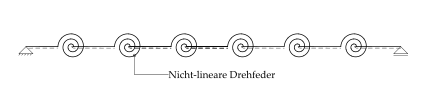
\includegraphics{index_files/mediabag/../imgs/Modell_Drehfeder.pdf}

}

\caption{\label{fig-modell_drehfeder}Federmodell, biege- und schubsteife
Stäbe gekoppelt mit Federn}

\end{figure}%

In dieser Modellierung resultieren sämtliche Verformungen des Systems
aus den Federverbindungen, welche in FE-Softwares als Stabendgelenke
modelliert werden können. Mit der Wahl der entsprechenden
Federcharakteristiken können passende Resultate erzielt werden. Dieser
Ansatz ermöglicht es, der Anzahl an Freiheitsgraden in den
Stabendgelenken entsprechend Steifigkeiten zuzuordnen. Den
Rotationsfreiheitsgraden werden Momenten-Verdrehungs-Beziehungen und den
Translationsfreiheitsgraden Kraft-Verformungs-Beziehungen zugeordnet. In
den betrachteten 3D-Statiksoftwares können den Stabendgelenken Verläufe
mittels eines Diagrammeditors eingegeben werden, die beliebige
nichtlineare Beziehungen abbilden, sofern diese numerisch stabil, sowie
stetig ansteigend sind. Grundsätzlich wird die
Momenten-Verdrehungs-Beziehung (Drehfedercharakteristik) anhand der
Momenten-Krümmungs-Beziehung des Querschnitts hergeleitet.
Schubverformungen lassen sich beispielsweise durch die Bestimmung einer
Kraft-Verformungs-Beziehung in Wirkungsrichtung der Querkraft ermitteln.
Es lässt sich vorwegnehmen, dass die Wahl der Federcharakteristiken die
Krux des Systems darstellt.

Alternativ zur Modellierung mittels Drehfedern lässt sich das Verhalten
der Drehfeder mit einem Wegfederpaar abbilden. Dies erlaubt eine
Modellierung mittels der nichtlinearen Fachwerksstäbe der Software
Statik-9 der Cubus AG. Dieser Ansatz wird nur im Einführungsbeispiel
berücksichtigt.

\begin{figure}[H]

\centering{

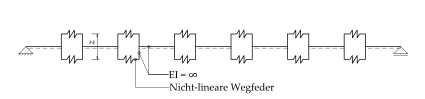
\includegraphics{index_files/mediabag/../imgs/Modell_Wegfeder.pdf}

}

\caption{\label{fig-modell_wegfeder}Federmodell, biege- und schubsteife
Stäbe gekoppelt mit einem Wegfederpaar}

\end{figure}%

\subsection{Modelleigenschaften}\label{modelleigenschaften}

Mit der Modellierung als Federmodell lassen sich beliebig komplexe
Stoffgesetze in einer praxisüblichen Statiksoftware anwenden. Speziell
können Biegeverformungen zuverlässig bestimmt werden, basierend auf der
Momenten-Krümmungs-Beziehung. Zudem lässt sich eine
Momenten-Krümmungs-Beziehung mit einer händischen Querschnittsanalyse
leicht verifizieren. Dies ermöglicht die Überprüfung der Resultate und
steigert so die Zuverlässigkeit der Berechnung. Ein weiterer Kernpunkt
der Modellierung ist die Berücksichtigung der Momentenumlagerung. Durch
die inkrementelle Steigerung der Last beim nichtlinearen
Berechnungsalgorithmus können Momente entsprechend der
beanspruchungsabhängigen Steifigkeit verteilt werden. Bei einem
Zweifeldträger kann beispielsweise die Last nach dem Erreichen des
Biegewiderstand beim Mittelauflager weiter gesteigert werden, sofern
ausreichend Verformungsvermögen vorhanden ist.

Ein konzeptioneller Nachteil der Modellbildung ist die Vielzahl an
Diskretisierungen. Dies gilt allgemein für numerische Lösungen. In
diesem Modell fliesst die Wahl der Elementlänge mit ein. Die
Inkrementgrösse zur Bestimmung der Momenten-Krümmungs-Beziehung, sofern
diese numerisch bestimmt wurde, hat einen Einfluss. Zudem gilt es bei
einer nichtlinearen Berechnung, eine Inkrementgrösse zur Steigerung der
Last im Lösungsalgorithmus zu wählen. Diese Parameter haben einen
Einfluss auf die Resultate und sind sorgfältig zu wählen.

\section{Einführungsbeispiel}\label{einfuxfchrungsbeispiel}

Das Einführungsbeispiel verfolgt das Ziel, das Modellverhalten
nachvollziehbar darzustellen. Dazu werden die Verformungen des fiktiven
Beispiels sowohl analytisch mittels der Arbeitsgleichung als auch
numerisch mit der Statiksoftware AxisVM-X7 ermittelt.

Als Beispiel wurde ein Kragarm gewählt, der mit einer Drehfeder versehen
ist, welche eine nichtlineare Drehfedercharakteristik aufweist. Es
werden zwei Laststufen betrachtet, die so gewählt sind, dass das
nichtlineare Verhalten der Drehfeder deutlich wird. Das statische System
ist in Abbildung~\ref{fig-kragarm-feder} dargestellt.

\begin{figure}[H]

\centering{

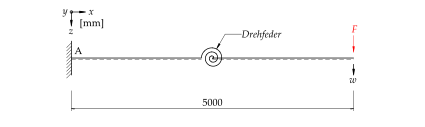
\includegraphics{index_files/mediabag/../imgs/Kragarm_system_Feder.pdf}

}

\caption{\label{fig-kragarm-feder}Statisches System des Kragarms,
versehen mit einer Drehfeder in Trägermitte}

\end{figure}%

Durch den Vergleich der analytischen und numerischen Ergebnisse wird die
Genauigkeit des Federmodells überprüft. Gleichzeitig bietet dieses
Beispiel eine klare und anschauliche Demonstration der
Modellierungsmethode, die im weiteren Verlauf der Arbeit auf komplexere
statische Systeme angewendet wird.

Die folgenden Parameter fliessen in die Berechnungen ein. Beschrieben
sind die Abmessungen und Materialeigenschaften, sowie die beiden
Laststufen \(F_1\) und \(F_2\), wie auch die Federsteifigkeiten
\(k_{\varphi1}\) und \(k_{\varphi2}\).

$$
\begin{aligned}
E &= 10000.0\ \frac{\mathrm{N}}{\mathrm{mm}^{2}} \; 
 &F_{1} &= -10000.0\ \mathrm{N} \; 
 &F_{2} &= -21500.0\ \mathrm{N} \; 
\\[11pt]
 h &= 400.0\ \mathrm{mm} \; 
 &k_{\varphi_{1}} &= 100000.0\ \frac{\mathrm{N} \cdot \mathrm{m}}{\mathrm{rad}} \; 
 &k_{\varphi_{2}} &= 10000.0\ \frac{\mathrm{N} \cdot \mathrm{m}}{\mathrm{rad}} \; 
\\[11pt]
 L &= 5.0\ \mathrm{m} \; 
 &z &= 400.0\ \mathrm{mm} \; 
 &b &= 200.0\ \mathrm{mm} \; 
\\[11pt]
\end{aligned}
$$

Das Beispiel wird mit einem Querschnitt versehen, der lediglich zur
Bestimmung der Biegesteifigkeit und folgend den Biegeverformungen dient.
Alternativ könnte der Kragarm biegestarr modelliert werden, da lediglich
die Verformungen aus der Drehfeder von Belang sind. Der
Rechteckquerschnitt, der für den gesamten Kragarm gilt, ist in
Abbildung~\ref{fig-qs-kragarm} dargestellt. Der Querschnitt ist mit
einem durchwegs linear-elastischem Materialverhalten versehen.

\begin{figure}[H]

\centering{

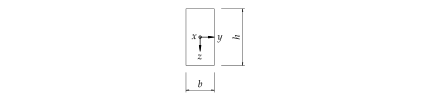
\includegraphics{index_files/mediabag/../imgs/Kragarm_querschnitt.pdf}

}

\caption{\label{fig-qs-kragarm}Rechteckquerschnitt des Kragarms mit
lokalem Koordinatensystem und Abmessungen}

\end{figure}%

Die Drehfedercharakteristik in globaler \(Y\)-Richtung, bezogen auf das
Koordinatensystem in Abbildung~\ref{fig-kragarm-feder}, ist in
Abbildung~\ref{fig-springcharacteristic} zu sehen. Das bilineare
Verhalten gilt für positive und negative Biegemomente und zeigt, wie die
Steifigkeit der Drehfeder sich ändert, wenn das Moment einen bestimmten
Schwellenwert überschreitet.

\begin{figure}[H]

\centering{

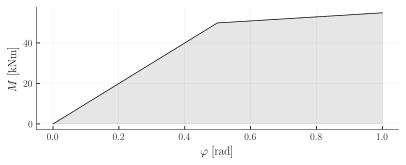
\includegraphics{index_files/mediabag/04_Kragarm_files/figure-pdf/fig-springcharacteristic-output-1.pdf}

}

\caption{\label{fig-springcharacteristic}Charakteristik der Drehfeder
des Kragarms}

\end{figure}%

\subsection{Biegeverformung}\label{biegeverformung}

Zunächst werden die Biegeverformungen mittels der Differentialgleichung
für reine Biegeträger ermittelt. Dabei wird die Drehfeder
vernachlässigt. Das statische System ist in
Abbildung~\ref{fig-kragarm-sys} dargestellt. Dieses Vorgehen führt zu
den Zustandslinien der Schnittgrössen, die in
Abbildung~\ref{fig-skkragarmreal} aufgezeigt sind.

\begin{figure}[H]

\centering{

\includegraphics{index_files/mediabag/../imgs/Kragarm_System.pdf}

}

\caption{\label{fig-kragarm-sys}Statisches System des Kragarms ohne
Drehfeder}

\end{figure}%

\begin{figure}[H]

\centering{

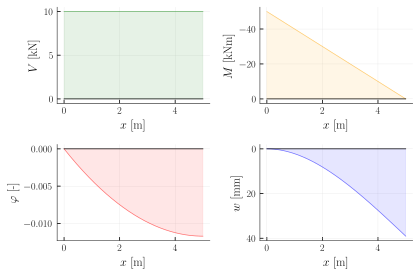
\includegraphics{index_files/mediabag/04_Kragarm_files/figure-pdf/fig-skkragarmreal-output-1.pdf}

}

\caption{\label{fig-skkragarmreal}Schnittkräfte des Systems aus
Abbildung~\ref{fig-kragarm-sys} für die Last \(F_1\)}

\end{figure}%

Die maximale Verformung am Endpunkt des Kragarms ohne Drehfeder beträgt:

$$
\begin{aligned}
w_{EI_{F1}} &= 39.1\ \mathrm{mm} \;
\end{aligned}
$$

Das analoge Vorgehen führt für die Laststufe \(F_2\) zu den
Zustandslinien der Schnittgrössen in der
Abbildung~\ref{fig-skkragarmreal_high}.

\begin{figure}[H]

\centering{

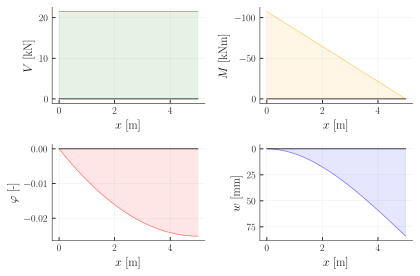
\includegraphics{index_files/mediabag/04_Kragarm_files/figure-pdf/fig-skkragarmreal_high-output-1.pdf}

}

\caption{\label{fig-skkragarmreal_high}Schnittkräfte des Systems aus
Abbildung~\ref{fig-kragarm-sys} für die Last \(F2\)}

\end{figure}%

Diese Darstellung zeigt, wie sich die Schnittgrössen des Kragarms unter
einer erhöhten Last ändern, und bietet eine Vergleichsbasis zur ersten
Laststufe \(F_1\). Da ein durchwegs linear-elastisches Biegeverhalten
vorausgesetzt wird, entspricht der Faktor der Erhöhung der Verformung
dem Quotienten der beiden Laststufen.

\[
\frac{w_{EI_{F2}}}{w_{EI_{F1}}} = \frac{F_2}{F_1}
\]

Dabei beträgt die maximale Biegeverformung am Ende des Kragarms ohne
Drehfeder für die Last \(F_2\):

$$
\begin{aligned}
w_{EI_{F2}} &= 84.0\ \mathrm{mm} \;
\end{aligned}
$$

\subsection{Verformung der Drehfeder}\label{verformung-der-drehfeder}

Zur Bestimmung der Verformung am Ende des Kragarms des Systems mit der
Drehfeder wird die Arbeitsgleichung angewendet. Dazu wird an einem
virtuellen System eine Einzellast eingeführt, an der Stelle an dem die
Verformung bestimmt werden soll. Dargestellt ist dies in
Abbildung~\ref{fig-kragarm-sys-virtuell}.

\begin{figure}[H]

\centering{

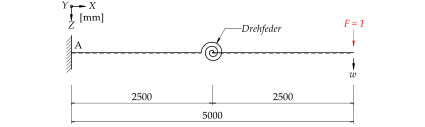
\includegraphics{index_files/mediabag/../imgs/Kragarm_system_feder_virtuell.pdf}

}

\caption{\label{fig-kragarm-sys-virtuell}Statisches System des Kragarms
im virtuellen Kräftezustand}

\end{figure}%

Die entsprechenden Verläufe der Querkraft und des Biegemoments zeigt die
Abbildung~\ref{fig-sk-kragarm-virtuell} für das virtuelle System.

\begin{figure}[H]

\centering{

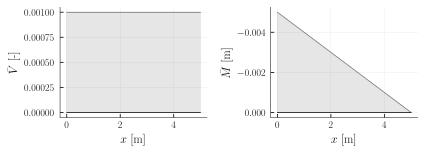
\includegraphics{index_files/mediabag/04_Kragarm_files/figure-pdf/fig-sk-kragarm-virtuell-output-1.pdf}

}

\caption{\label{fig-sk-kragarm-virtuell}Schnittkräfte des virtuellen
Systems aus Abbildung~\ref{fig-kragarm-sys-virtuell}}

\end{figure}%

Bei der Arbeitsgleichung werden lediglich Verdrehungsterme
berücksichtigt. Die Verformung der Drehfeder kann somit mit der
folgenden Gleichung bestimmt werden.

\[
w_{\varphi} = \bar{M} \frac{M}{k_\varphi} = \bar{M} \varphi
\]

Die Verdrehung lässt sich aus der Federcharakteristik mit dem
Biegemoment in Trägermitte bestimmen. Die
Abbildung~\ref{fig-feder-force} zeigt die Position der Laststufen im
Diagramm.

\begin{figure}[H]

\centering{

\includegraphics{index_files/mediabag/04_Kragarm_files/figure-pdf/fig-feder-force-output-1.pdf}

}

\caption{\label{fig-feder-force}Charakteristik der Drehfeder mit
Bestimmung der Verdrehung anhand der Laststufen}

\end{figure}%

Angewendet auf das System der Abbildung~\ref{fig-kragarm-feder} folgen
für die beiden Laststufen die Deformationen der Drehfeder zu:

$$
\begin{aligned}
w_{\varphi_{F1}} &= 625.0\ \mathrm{mm} \; 
 &w_{\varphi_{F2}} &= 2201.3\ \mathrm{mm} \;
\end{aligned}
$$

Dazu gilt es den Anteil aus der Biegeverformung zu addieren. Die totale
Verformung beträgt:

$$
\begin{aligned}
w_{F1} &= w_{\varphi_{F1}} + w_{EI_{F1}}  = 625.0\ \mathrm{mm} + 39.1\ \mathrm{mm} &= 664.1\ \mathrm{mm}  
\\[11pt]
w_{F2} &= w_{\varphi_{F2}} + w_{EI_{F2}}  = 2201.3\ \mathrm{mm} + 84.0\ \mathrm{mm} &= 2285.2\ \mathrm{mm}  
\end{aligned}
$$

\subsection{Stabstatikmodell}\label{stabstatikmodell}

Die analytisch ermittelten Verformungen werden nun mit der Lösung der
Stabstatiksoftware verglichen. Das statische System, gemäss
Abbildung~\ref{fig-kragarm-feder}, wird in der Statiksoftware AxisVM X7
modelliert. Dazu wird die Drehfeder als Federelement modelliert und in
der \(Y\)-Dimension mit der Federcharakteristik versehen. Die
angeschlossenen Stäbe sind mit entsprechendem Querschnitt und der
entsprechenden Biegesteifigkeit modelliert. Die Verformungen in
\(Z\)-Richtung sind in Abbildung~\ref{fig-kragarm-drehfeder-10} und
Abbildung~\ref{fig-kragarm-drehfeder-215} gezeigt.

\begin{figure}[H]

\centering{

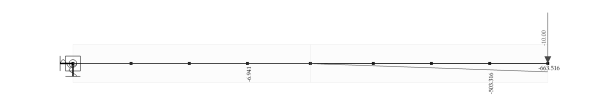
\includegraphics{index_files/mediabag/../imgs/Kragarm_drehfeder_10.pdf}

}

\caption{\label{fig-kragarm-drehfeder-10}Verformungen in \(Z\)-Richtung
für \(F_1\) aus AxisVM-X7 mit dem Federmodell}

\end{figure}%

Das Modell liefert für die Last \(F_1\) die maximale Verformung aus der
Drehfeder und dem Biegestab von:

\[
w_{1,tot,F1} = 663.5 \text{mm}
\]

\begin{figure}[H]

\centering{

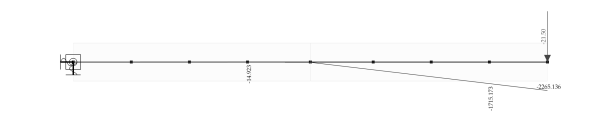
\includegraphics{index_files/mediabag/../imgs/Kragarm_drehfeder_215.pdf}

}

\caption{\label{fig-kragarm-drehfeder-215}Verformungen in \(Z\)-Richtung
für \(F_2\) aus AxisVM-X7 mit dem Federmodell}

\end{figure}%

Für die Last \(F_2\) beträgt die maximale Gesamtverformung:

\[
w_{1,tot,F2} = 2265.1 \text{mm}
\]

Das Modell liefert die annähernd gleichen Resultate wie die
Handrechnung. Die Genauigkeit ist zufriedenstellend.

\subsubsection{Modellierungsalternative
Wegfeder}\label{modellierungsalternative-wegfeder}

Wie bereits in Kapitel~\ref{sec-modellvorstellung} erläutert, lässt sich
das Verhalten der Drehfeder mit einem Wegfederpaar abbilden. Dazu wird
in einem ersten Schritt die Drehfedercharakteristik in eine
Wegfedercharakteristik umgerechnet. Als Grundlage dient die Modellierung
gemäss Abbildung~\ref{fig-verdrehung_verformung}. Die Abbildung zeigt
die kinematische Relation eines reinen Biegeelements.

\begin{figure}[H]

\centering{

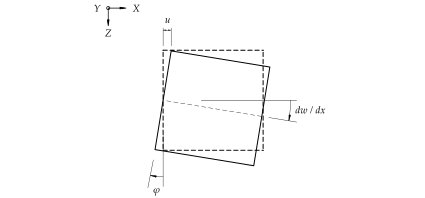
\includegraphics{index_files/mediabag/../imgs/Skizze_Verdrehung_Verformung.pdf}

}

\caption{\label{fig-verdrehung_verformung}Kinematische Relation eines
reinen Biegeelements}

\end{figure}%

Mittels den folgenden Gleichungen lässt sich so die
Wegfedercharakteristik bestimmen. Der Abstand zwischen dem Wegfederpaar
wird mit \(z\) beschrieben.

\[
F = \frac{M}{z}
\]

\[
u = \frac{\tan(\varphi) \cdot z}{2} \simeq \frac{\varphi \cdot z}{2}
\]

Durch die Berücksichtigung der trigonometrischen Funktion ist der
Verlauf nicht exakt bilinear. Die umgerechnete Wegfedercharakteristik
ist in Abbildung~\ref{fig-wegfeder-force} aufgezeigt. Der Verlauf kann
lediglich mit einer begrenzten Anzahl an Punkten im Diagrammeditor von
AxisVM-X7 hinterlegt werden. Dies ist gleichbedeutend mit einer
Diskretisierung des Verlaufs.

\begin{figure}[H]

\centering{

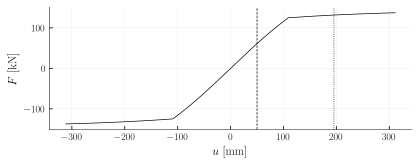
\includegraphics{index_files/mediabag/04_Kragarm_files/figure-pdf/fig-wegfeder-force-output-1.pdf}

}

\caption{\label{fig-wegfeder-force}Charakteristik der Wegfeder,
umgerechnet aus der Drehfedercharakteristik}

\end{figure}%

Die Resultate mit dem Wegfedermodell sind in der
Abbildung~\ref{fig-f1-wegfeder} und Abbildung~\ref{fig-f2-wegfeder}
gezeigt.

\begin{figure}[H]

\centering{

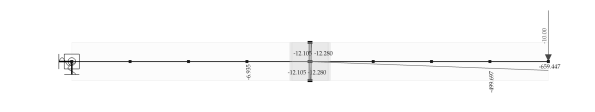
\includegraphics{index_files/mediabag/../imgs/Kragarm_wegfeder_10.pdf}

}

\caption{\label{fig-f1-wegfeder}Verformungen in \(Z\)-Richtung für
\(F_1\) aus AxisVM-X7 mit Wegfedermodell}

\end{figure}%

Die maximale Verformung in \(Z\)-Richtung für die Last \(F_1\)
entspricht:

\[
w_{1,tot,F1} = 659 \text{mm}
\]

Und für die Last \(F_2\):

\[
w_{1,tot,F2} = 2137.8 \text{mm}
\]

\begin{figure}[H]

\centering{

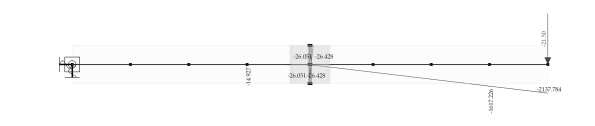
\includegraphics{index_files/mediabag/../imgs/Kragarm_wegfeder_215.pdf}

}

\caption{\label{fig-f2-wegfeder}Verformungen in \(Z\)-Richtung für
\(F_2\) aus AxisVM-X7 mit Wegfedermodell}

\end{figure}%

Die Resultate der Modellierung mittels Wegfedern zeigen Differenzen zu
denen mit der Drehfeder. Dies lässt sich auf die Diskretisierung des
nichtlinearen Verlaufs der Wegfedercharakteristik zurückführen. Eine
Approximation des Verlaufs führt zu beträchtlichen Abweichungen im
Bereich der zweiten Laststufe. Dies ist auf die geringe Neigung, bzw.
auf die Grösse von \(k_{\varphi_2}\) der Drehfedercharakteristik
zurückzuführen.

Das Einführungsbeispiel zeigt wie das Biegeverhalten durch die Drehfeder
beeinflusst wird. Die Verformungsgrösse ist unter Vernachlässigung der
Stabverformungen direkt abhängig von der Federcharakteristik. Dies
ermöglicht eine gezielte Steuerung der Verformungen. Zudem ist die
Nachvollziehbarkeit durch die direkte Abhängigkeit gegeben. Das
nichtlineare Verhalten ist problemlos modellierbar. Ebenfalls
veranschaulicht das Beispiel, speziell die Modellierungsalternative, die
Problematik der Diskterisierung, angesprochen in
Kapitel~\ref{sec-modellvorstellung}.

\bookmarksetup{startatroot}

\chapter{Modellverifizierung}\label{sec-verifizierung}

Das vorangegangen Kapitel beschreibt das Konzept des Federmodells und
liefert anhand des Einführungsbeispiel einen nachvollziehbaren
Berechnungsablauf. Um sich von der Betrachtung eines fiktiven Beispiels
zu lösen, wird in diesem Kapitel die Anwendung des Federmodells auf die
beiden Versuche der Vertiefungsarbeit I
{[}\citeproc{ref-gitz_ansatze_2024}{1}{]} beschrieben. Es sind die
relevanten Versuchsgrundlagen aufgezeigt. Detaillierte Beschriebe sind
aus {[}\citeproc{ref-gitz_ansatze_2024}{1}{]} und der darin verwiesenen
Literatur zu entnehmen.

Der Dreipunkbiegeversuch zeigt die Anwendung des Federmodells zur
Bestimmung der Biegeverformungen und der Schubverformungen. Dabei wird
die Ermittlung der Biege- und Schubsteifigkeit aufgezeigt. Der
Vierpunktbiegeversuch greift dieselben Thematiken auf. Ergänzt wird der
Versuch mit der Modellierung des Versatzmass. Das Versatzmass beschreibt
den Einfluss der Längszugkraft infolge der Querkraft. Es wird erwartet,
dass das Federmodell die gleichen Resultate wie die Berechnungen in der
Vertiefungsarbeit I liefern.

\section{Dreipunktbiegeversuch}\label{dreipunktbiegeversuch}

Der Dreipunktbiegeversuch wurde aus der Versuchsserie
{[}\citeproc{ref-jager_versuche_2006}{2}{]} entnommen. Es handelt sich
um den dritten Versuch der Versuchsserie A in der zweiten
Versuchsanordnung, kurz betitelt mit A3V2. Der Versuch wurde gewählt, da
vor dem Biegeversagen ein deutliches Fliessen der Längsbewehrung
gemessen wurde. Zudem war die saubere Dokumentation ein
ausschlaggebender Faktor.

\subsection{Versuchsbeschrieb}\label{versuchsbeschrieb}

Der Versuchsaufbau ist in der Abbildung~\ref{fig-anordnung_a3v2}
gezeigt. Der Plattenstreifen ist auf einem Punktlager horizontal und
vertikal unverschieblich gelagert. Das zweite Lager bildet eine Presse.
Die Lagerung der Presse gilt als horizontal verschieblich.

\begin{figure}[H]

\centering{

\includegraphics{index_files/mediabag/../imgs/versuchsanordnung_A3V2.pdf}

}

\caption{\label{fig-anordnung_a3v2}Versuchsanordnung des
Dreipunktbiegeversuchs, Zeichnung entnommen aus
{[}\citeproc{ref-jager_versuche_2006}{2}{]}}

\end{figure}%

Der Querschnitt des Plattenstreifens ist in Abbildung~\ref{fig-qs_a3v2}
gezeigt. Das Bewehrungslayout in Querrichtung ist dargestellt. Der
Querschnitt ist mit entsprechenden Abmessungen versehen.

\begin{figure}[H]

\centering{

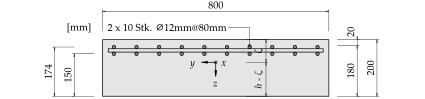
\includegraphics{index_files/mediabag/../imgs/QS_Versuch_A3.pdf}

}

\caption{\label{fig-qs_a3v2}Querschnitt des Dreipunktbiegeversuchs,
Zeichnung entnommen aus {[}\citeproc{ref-gitz_ansatze_2024}{1}{]}}

\end{figure}%

Das Bewehrungslayout in Längsrichtung ist in der
Abbildung~\ref{fig-bewehrung_a3v2} aufgezeigt. Der Plattenstreifen ist
mit einer durchgehenden Längsbewehrung in der Zugzone bewehrt. Verankert
ist die Längsbewehrung mit angeschweissten Platten. Die Schubdübel sind
nicht durchgängig verlegt. Der letzte Bereich des Versuchskörper weist
keine Schubbewehrung auf.

\begin{figure}[H]

\centering{

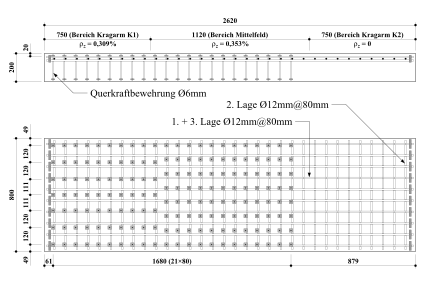
\includegraphics{index_files/mediabag/../imgs/bewehrung_a3v2.pdf}

}

\caption{\label{fig-bewehrung_a3v2}Bewehrungslayout des
Dreipunktbiegeversuchs, Zeichnung entnommen aus
{[}\citeproc{ref-jager_versuche_2006}{2}{]}}

\end{figure}%

\subsubsection{Versuchsergebnisse}\label{versuchsergebnisse}

Der Abschluss des Versuchsbeschriebs bilden die Versuchsergebnisse.
Beschrieben werden die Messresultate, sowie der Belastungshergang. Der
Plattenstreifen wurde in der ersten Versuchsanordnung bereits
vorbelastet. Nach der Vorbelastung drehte man den Träger und brachte ihn
in die neue Anordnung. Darauf folgte die Belastung mit der Einzellast
\(F_A\). Der Versuchskörper wurde weggesteuert bis zum Bruch gefahren.
Die Aufzeichnung der Verformungen begann ab dem Belastungsbegin der
Pressen. Die Abbildung~\ref{fig-verformungslinie_a3v2} zeigt die
Verformung entlang der Stabachse für die entsprechenden Laststufen. Das
Last-Verformungs-Diagramm an der Stelle der Lasteinleitung ist in der
Abbildung~\ref{fig-last_verformung_a3v2} aufgezeigt. Die Traglast des
Systems lag bei circa \(320\) kN.

\begin{figure}[H]

\centering{

\includegraphics{index_files/mediabag/../imgs/a3v2_verformungsverlauf.pdf}

}

\caption{\label{fig-verformungslinie_a3v2}Verformungsverlauf des
Dreipunktbiegeversuchs, Zeichnung entnommen aus
{[}\citeproc{ref-jager_versuche_2006}{2}{]}}

\end{figure}%

\begin{figure}[H]

\centering{

\includegraphics{index_files/mediabag/../imgs/a3v2_last_verformung_Fa.pdf}

}

\caption{\label{fig-last_verformung_a3v2}Last-Verformungs-Diagramm des
Dreipunktbiegeversuchs, Zeichnung entnommen aus
{[}\citeproc{ref-jager_versuche_2006}{2}{]}}

\end{figure}%

\subsection{Modellierung}\label{modellierung}

In diesem Abschnitt wird die Modellierung des Systems aufgezeigt. Das
Ziel ist es das Verhalten des Versuchskörpers mit einem simplen Modell
abzubilden. Das statische System des Versuchs ist in
Abbildung~\ref{fig-system_a3v2} dargestellt. Das Eigengewicht wird
vernachlässigt, da die Verformungsmessungen nach dem Einbau des Versuchs
beginnen.

\begin{figure}[H]

\centering{

\includegraphics{index_files/mediabag/../imgs/A3V2_system.pdf}

}

\caption{\label{fig-system_a3v2}Statisches System des
Dreipunktbiegeversuchs}

\end{figure}%

Die Auflagerbreiten werden vernachlässigt. Auf die Darstellung der
Federn wird verzichtet. Diese sind in einem Abstand von \(10\) mm
entlang der Stabachse verteilt.

$$
\begin{aligned}
l_{E} &= 10.0\ \mathrm{mm} \; \;\textrm{(Elementlänge des biege- und schubsteifen Stabs)}
\end{aligned}
$$

Der Einfluss der Elementlänge wurde mittels einer Sensitivitätsanalyse
ermittelt. Eine feinere Stabunterteilung resultiert zu keiner
signifikanten Änderung der Resultate.

\subsubsection{Biegeverformungen}\label{biegeverformungen}

Dieser Abschnitt beschreibt die Ermittlung der Biegesteifigkeit des
Systems. Zur Bestimmung der Biegeverformungen ist eine
Drehfedercharakteristik zu definieren. Dazu wird anhand einer
Querschnittsanalyse eine Momenten-Krümmungs-Beziehung ermittelt. Durch
Multiplikation der Krümmung mit der Elementlänge resultiert eine
Momenten-Verdrehungs-Beziehung, sprich eine Drehfedercharakteristik. Die
Querschnittsanalyse basiert auf einem bilinearen
Spannungs-Dehnungs-Verhalten für den Betonstahl. Der Beton wird mittels
einem linear-elastischen ideal plastischen Werkstoffgesetz
berücksichtigt. Dies resultiert zu der bilinearen Beziehung gemäss der
Abbildung~\ref{fig-mchi_a3v2}. Detaillierte Berechnungen sind in der
Vertiefungsarbeit I {[}\citeproc{ref-gitz_ansatze_2024}{1}{]} zu finden.
In der Vertiefungsarbeit I wurde die Zugfestigkeit des Betons
mitberücksichtigt. Diese wird in dieser Analyse aufgrund von
Konvergenzproblemen im numerischen Modell vernachlässigt.

\begin{figure}[H]

\centering{

\includegraphics{index_files/mediabag/05_Versuchsnachrechnung_VM1_files/figure-pdf/fig-mchi_a3v2-output-1.pdf}

}

\caption{\label{fig-mchi_a3v2}Momenten-Krümmungs-Beziehung des
Dreipunktbiegeversuchs, ohne ungerissenen Bereich, übernommen aus
{[}\citeproc{ref-gitz_ansatze_2024}{1}{]}}

\end{figure}%

Die Ableitung der Momenten-Krümmungs-Beziehung nach der Krümmung
entspricht der Biegesteifigkeit. Der bilineare Verlauf zeigt eine
Biegesteifigkeit für den gerissenen Querschnitt. Der zweite Bereich
beschreibt die Biegesteifigkeit für den Zustand des Fliessens der
Bewehrung. Im gerissenen Bereich kann die Steifigkeit durch die
Zugversteifung erhöht werden. Diese berücksichtigt das Mitwirken des
Betons zwischen den Rissen.

Die daraus resultierende Momenten-Verdrehungs-Beziehung ist in der
Abbildung~\ref{fig-mphi_a3v2} aufgezeigt. Diese ist den Stabendgelenken
als Drehfedercharakteristik in globaler \(Y\)-Richtung, gemäss
Abbildung~\ref{fig-system_a3v2}, zu hinterlegen.

\begin{figure}[H]

\centering{

\includegraphics{index_files/mediabag/05_Versuchsnachrechnung_VM1_files/figure-pdf/fig-mphi_a3v2-output-1.pdf}

}

\caption{\label{fig-mphi_a3v2}Momenten-Verdrehungs-Beziehung des
Dreipunktbiegeversuchs}

\end{figure}%

\subsubsection{Schubverformungen}\label{schubverformungen}

Die Bestimmung der Schubsteifigkeit der einzelnen Federn wird in diesem
Abschnitt aufgezeigt. Zuerst wird das Vorgehen beschrieben, danach wird
die betragsmässige Ermittlung gezeigt.

Die Schubsteifigkeit wird mittels einer Wegfedercharakteristik
beschrieben. Diese wird in globaler \(Z\)-Richtung, entsprechend dem
Koordinatensystem aus Abbildung~\ref{fig-system_a3v2}, bestimmt. Dabei
wird ein Kraftfluss entsprechend den Spannungsfeldern in
Abbildung~\ref{fig-spannungsfelder_a3v2} angenommen. Es wird
vorausgesetzt, dass lediglich die Schubbewehrung Querkräfte aufnimmt.
Ein Mitwirken des Betons wird nicht berücksichtigt. Anhand der
Beanspruchung der Schubbewehrung kann deren Verformung ermittelt werden.
Daraus resultiert eine Kraft-Verformungs-Beziehung.

\begin{figure}[H]

\centering{

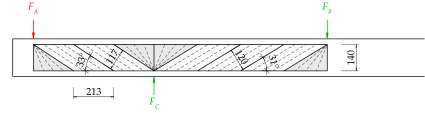
\includegraphics{index_files/mediabag/../imgs/Spannungsfelder_flach.pdf}

}

\caption{\label{fig-spannungsfelder_a3v2}Einteilung in Spannungsfelder
des Dreipunktbiegeversuchs, Zeichnung entnommen aus
{[}\citeproc{ref-gitz_ansatze_2024}{1}{]}}

\end{figure}%

Dazu wird die Anzahl an mitwirkenden Schubdübeln pro Spannungsfeld
bestimmt. Die Schubdübel weisen das Spannungs-Dehnungs-Verhalten gemäss
der Abbildung~\ref{fig-sigma-eps-a3v2} auf. Die Kraftkomponente ergibt
sich aus der Querschnittsfläche der mitwirkenden Dübel multipliziert mit
der Zugfestigkeit. Die Verformung wird mittels Multiplikation der
Dehnungen aus der Spannungs-Dehnungs-Beziehung mit dem Hebelarm der
inneren Kräfte bestimmt. Die bestimmte Wegfedercharakteristik gilt für
das betrachtete Spannungsfeld. Abschliessend wird die Verformung um den
Faktor gemäss folgender Gleichung reduziert.

\[
\gamma_{E} = \frac{z \cdot \cot(\theta)}{l_{E}}
\]

\(l_{E}\) steht für Elementlänge

Diese erhöht die Steifigkeit jeder Feder. In der Summe bilden die
Verformungen der einzelnen Federn innerhalb des Spannungsfelds die
gesamte Verformung des Spannungsfelds ab.

\begin{figure}[H]

\centering{

\includegraphics{index_files/mediabag/05_Versuchsnachrechnung_VM1_files/figure-pdf/fig-sigma-eps-a3v2-output-1.pdf}

}

\caption{\label{fig-sigma-eps-a3v2}Spannungs-Dehnungs-Beziehung der
Schubbewehrung, übernommen aus
{[}\citeproc{ref-gitz_ansatze_2024}{1}{]}}

\end{figure}%

Folgend sind die Parameter zur Bestimmung der Wegfedercharakteristik
gezeigt. Der gewählte Neigungswinkel der Spannungsfelder \(\theta_{c3}\)
gilt für den Bruchzustand. Vereinfacht wird die daraus bestimmte
Wegfedercharakteristik für sämtliche Laststufen angesetzt. Dies führt zu
Abweichungen des Verformungsverhalten im Lastniveau unterhalb der
Traglast.

$$
\begin{aligned}
\oslash_{sw} &= 6.0\ \mathrm{mm} \; 
 &S_{sw} &= 80.0\ \mathrm{mm} \; 
 &b_{w} &= 800.0\ \mathrm{mm} \; 
\\[12pt]
 E_{sw} &= 205000.0\ \frac{\mathrm{N}}{\mathrm{mm}^{2}} \; 
 &z &= 140.0\ \mathrm{mm} \; 
 &\theta_{c3} &= 34.3\ \mathrm{°} \; 
\\[12pt]
 f_{su} &= 630.0\ \frac{\mathrm{N}}{\mathrm{mm}^{2}} \;
\end{aligned}
$$

In einem ersten Schritt wird die Querschnittsfläche der Schubbewehrung
bestimmt. Gemäss der Abbildung~\ref{fig-bewehrung_a3v2} ist ersichtlich,
dass entlang der Plattenbreite \(7\) Schubdübel verlegt sind. Die
Querschnittsfläche für eine Dübelreihe folgt somit zu:

$$
\begin{aligned}
A_{sw} &= 7 \cdot \left( \frac{ \oslash_{sw} }{ 2 } \right) ^{ 2 } \cdot \pi \; 
\end{aligned}
$$

$$
\begin{aligned}
A_{sw} &= 197.9\ \mathrm{mm}^{2} \;
\end{aligned}
$$

Wird diese nun über einen Meterstreifen verschmiert, so folgt:

$$
\begin{aligned}
a_{sw} &= \frac{ A_{sw} }{ S_{sw} } \; 
\end{aligned}
$$

$$
\begin{aligned}
a_{sw} &= 2474.0\ \frac{\mathrm{mm}^{2}}{\mathrm{m}} \;
\end{aligned}
$$

Darauf folgt die Bestimmung des Querkraftwiderstands. Gemäss der
Abbildung~\ref{fig-last_verformung_a3v2} ist ersichtlich, dass der
Plattenstreifen bei \(320\) kN versagt. Der Querkraftwiderstand muss der
Querkraft unter der Traglast entsprechen. Folglich ist zu kontrollieren,
ob sich mittels des gewählten Neigungswinkels \(\theta_{c3}\) der
geforderte Querkraftwiderstand einstellt.

$$
\begin{aligned}
V_{R} &= a_{sw} \cdot z \cdot \frac{ f_{su} }{ \tan \left( \theta_{c3} \right) } \; 
\end{aligned}
$$

$$
\begin{aligned}
V_{R} &= 319.9\ \mathrm{kN} \;
\end{aligned}
$$

Der Querkraftwiderstand entspricht in etwa der Querkraft aus der
Traglast. Die Wegfedercharakteristik lässt sich abschliessend unter
Berücksichtigung des Reduktionsfaktors ermitteln. Die Berechnung des
Reduktionsfaktors ist folgend gezeigt:

$$
\begin{aligned}
\gamma_{E} &= z \cdot \frac{ 1 }{ \tan \left( \theta_{c3} \right) } \cdot \frac{1} { l_{E} }  = 140\ \mathrm{mm} \cdot \frac{ 1 }{ \tan \left( 34\ \mathrm{°} \right) } \cdot \frac{1} { 10\ \mathrm{mm} } &= 21\  
\end{aligned}
$$

Die Abbildung~\ref{fig-wegfeder-schub-a3v2} zeigt das ermittelte
Kraft-Verformungs-Verhalten. Das Verhalten ist analog dem bilinearen
Spannungs-Dehnungs-Diagramm. Dies wird den Federn in globaler
\(Z\)-Richtung hinterlegt.

\begin{figure}[H]

\centering{

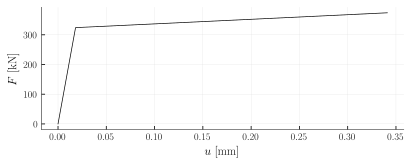
\includegraphics{index_files/mediabag/05_Versuchsnachrechnung_VM1_files/figure-pdf/fig-wegfeder-schub-a3v2-output-1.pdf}

}

\caption{\label{fig-wegfeder-schub-a3v2}Berechnete
Wegfedercharakteristik der Federn in \(Z\)-Richtung des
Dreipunktbiegeversuchs}

\end{figure}%

\subsection{Modellergebnisse}\label{modellergebnisse}

Mit den bestimmten Federcharakteristiken kann die Verformungslinie des
Systems ermittelt werden. Das Modell ist in der Lage, Biege- und
Schubverformungen zu beschreiben, basierend auf nichtlinearen
Stoffgesetzen.

Die Abbildung~\ref{fig-fwa3v2} zeigt das Last-Verformungs-Diagramm des
Systems bei der Lasteinleitung. Gezeigt sind die Resultate des Modells,
mit und ohne Berücksichtigung der Zugversteifung, sowie die gemessenen
Versuchsresultate aus dem Versuchsbericht.

\begin{figure}[H]

\centering{

\includegraphics{index_files/mediabag/05_Versuchsnachrechnung_VM1_files/figure-pdf/fig-fwa3v2-output-1.pdf}

}

\caption{\label{fig-fwa3v2}Last-Verformungs-Verlauf an der Stelle der
Lasteinleitung aus dem Federmodell und aus den Versuchsmessungen}

\end{figure}%

Der Verdrehungsverlauf in Abbildung~\ref{fig-phi-max-a3v2} lässt sich
ebenfalls direkt aus dem Modell exportieren. Durch die Ableitung des
Verlaufs resultiert der Krümmungsverlauf.

\begin{figure}[H]

\centering{

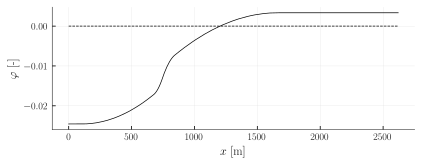
\includegraphics{index_files/mediabag/05_Versuchsnachrechnung_VM1_files/figure-pdf/fig-phi-max-a3v2-output-1.pdf}

}

\caption{\label{fig-phi-max-a3v2}Verdrehungsverlauf aus dem Federmodell
für die Traglast}

\end{figure}%

Der Krümmungsverlauf in der Abbildung~\ref{fig-chi-max-a3v2} gibt
Aufschluss über die Steifigkeit des Plattenstreifens entlang der
Stabachse. Beim Auflager \(C\) fliesst die Längsbewehrung. Der
dreieckige Verlauf neben dem Auflager \(C\) beschreibt den gerissenen
Bereich.

\begin{figure}[H]

\centering{

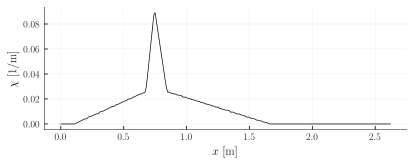
\includegraphics{index_files/mediabag/05_Versuchsnachrechnung_VM1_files/figure-pdf/fig-chi-max-a3v2-output-1.pdf}

}

\caption{\label{fig-chi-max-a3v2}Berechneter Krümmungsverlauf aus dem
Verdrehungsverlauf}

\end{figure}%

Das Modell beschreibt den Verformungsverlauf zufriedenstellend. Die
Resultate sind deckungsgleich mit den Modellresultaten aus der
Vorarbeit. Die Verifizierung des Modells am Dreipunktbiegeversuch wird
als gelungen betrachtet.

\newpage{}

\section{Vierpunktbiegeversuch}\label{vierpunktbiegeversuch}

Der Vierpunktbiegeversuch, kurz SV14, wurde aus der Publikation
{[}\citeproc{ref-tue_einfluss_2019}{3}{]} entnommen. Auffallend bei
diesem Versuch ist die niedrig gehaltene Schubbewehrung. Der Versuch
wurde gewählt, um den Einfluss der Schubverformungen in den Vordergrund
zu bringen.

\subsection{Versuchsbeschrieb}\label{versuchsbeschrieb-1}

Es handelt sich um einen Träger mit rechteckigem Querschnitt, gelagert
als einfacher Balken. In Längsrichtung sind Stäbe mit unterschiedlicher
Güte verlegt. In der Publikation sind zum Beton und den beiden
Betonstählen keine umfassenden Materialprüfungen beschrieben.

\begin{figure}[H]

\centering{

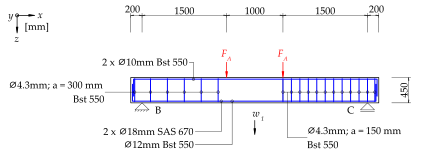
\includegraphics{index_files/mediabag/../imgs/versuchsskizze_14.pdf}

}

\caption{\label{fig-versuchsskizze-SV14}Bewehrungslayout des
Vierpunktbiegeversuchs, Zeichnung entnommen aus
{[}\citeproc{ref-gitz_ansatze_2024}{1}{]}}

\end{figure}%

Die Abbildung~\ref{fig-versuchsskizze-SV14} zeigt die Lagerung des
Trägers, sowie die Stellen der Lasteinleitung. Zusätzlich ist das
Bewehrungslayout dargestellt. Die Längsbewehrung ist stossfrei verlegt.
Am Ende ist diese abgebogen. Dies dient zur Verankerung. Der
Schubbewehrungsgehalt unterscheidet sich für die beiden Trägerhälften.

Die Abbildung~\ref{fig-QS-SV14} zeigt den Querschnitt mit den
Hauptabmessungen. Die Position der Längsbewehrung ist vermasst. Sowie
sind die Hauptabmessungen dargestellt.

\begin{figure}[H]

\centering{

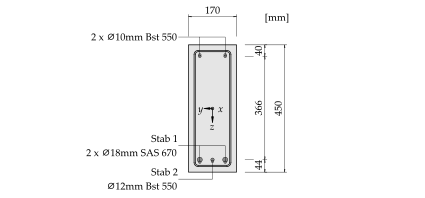
\includegraphics{index_files/mediabag/../imgs/QS_Versuch14.pdf}

}

\caption{\label{fig-QS-SV14}Querschnitt des Vierpunktbiegeversuchs,
nachgezeichnet nach {[}\citeproc{ref-gitz_ansatze_2024}{1}{]}}

\end{figure}%

\subsubsection{Versuchsergebnisse}\label{versuchsergebnisse-1}

Belastet wurde der Träger an beiden Stellen \(F_A\) bis zum Versagen.
Aufgrund des unterschiedlichen Schubbewehrungsgehalts erfolgte zuerst
ein Schubversagen in der schwächer bewehrten Zone. Diese wurde
nachträglich verstärkt. Abschliessend wurde die Last gesteigert, bis ein
Biegeversagen in der Feldmitte eintrat. Gemessen wurden die Verformungen
an der Stelle \(w_1\). Die Abbildung~\ref{fig-sv14_versuchsres_1} zeigt
das Rissbild nach dem Schubversagen der schwächer bewehrten Zone.

\begin{figure}[H]

\centering{

\includegraphics{index_files/mediabag/../imgs/sv14_versuchsresultat1.pdf}

}

\caption{\label{fig-sv14_versuchsres_1}Rissbild des
Vierpunktbiegeversuchs nach dem Versagen der schwächeren Zone, entnommen
aus {[}\citeproc{ref-tue_einfluss_2019}{3}{]}}

\end{figure}%

Die Abbildung~\ref{fig-sv14_versuchsres_2} zeigt einen Ausschnitt der
Last-Verformungs-Diagramme der Versuche der Serie. Rechts ist der
Versuch SV14 abgebildet. Die nachträgliche Verstärkung ist dargestellt,
sowie die Stelle des Biegeversagens. Die Traglast beträgt circa \(105\)
kN.

\begin{figure}[H]

\centering{

\includegraphics{index_files/mediabag/../imgs/sv14_versuchsresultat_2.pdf}

}

\caption{\label{fig-sv14_versuchsres_2}Last-Verformungs-Diagramm für
einen Teil der Versuchsserie, Versuch SV14 rechts, entnommen aus
{[}\citeproc{ref-tue_einfluss_2019}{3}{]}}

\end{figure}%

\subsection{Modellierung}\label{modellierung-1}

In diesem Abschnitt wird auf die Modellierung des Versuchs eingegangen.
Das statische System ist in der Abbildung~\ref{fig-system-SV14} gezeigt.
Die Auflagerbreite wird vernachlässigt. Die Versuchsmessung der
Durchbiegungen zeigt, dass die Verformung bei Lastbeginn null ist. Dies
führt zur Annahme, dass der Einfluss des Eigengewichts nicht gemessen
wurde. Somit wird dieses vernachlässigt.

\begin{figure}[H]

\centering{

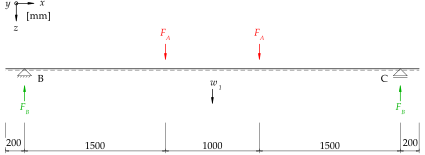
\includegraphics{index_files/mediabag/../imgs/statisches_system_14.pdf}

}

\caption{\label{fig-system-SV14}Statisches System des
Vierpunktbiegeversuchs, Zeichnung entnommen aus
{[}\citeproc{ref-gitz_ansatze_2024}{1}{]}}

\end{figure}%

Auf die Darstellung der Federn wird verzichtet. Diese sind in einem
Abstand von \(10\) mm entlang der Stabachse verteilt.

$$
\begin{aligned}
l_{E} &= 10.0\ \mathrm{mm} \; \;\textrm{(Elementlänge des biege- und schubsteifen Stabs)}
\end{aligned}
$$

Analog zum Vorgehen beim Dreipunktbiegeversuch wurde die Elementlänge
mittels einer Sensitivitätsanalyse ermittelt. Eine feinere
Stabunterteilung bewirkt keine aussagekräftige Änderung der Resultate.

\subsubsection{Biegeverformungen}\label{biegeverformungen-1}

Wie beim Dreipunktbiegeversuch wird zuerst die Biegesteifigkeit des
Systems ermittelt. Dazu wird die Drehfedercharakteristik der Federn
bestimmt. Die Grundlage der Drehfedercharakteristik bildet die
Momenten-Krümmungs-Beziehung. Für den Querschnitt des
Vierpunktbiegeversuchs gilt die Beziehung gemäss
Abbildung~\ref{fig-mchi_sv14}. Für detaillierte Berechnungen ist die
Vertiefungsarbeit I {[}\citeproc{ref-gitz_ansatze_2024}{1}{]} zu
konsultieren. Die Beziehung wurde basierend auf bilinearen
Spannungs-Dehnungs-Beziehungen für den Betonstahl und linear-elastischen
ideal-plastischen Spannungs-Dehnungs-Beziehungen für den Beton bestimmt.
Die Zugfestigkeit des Betons wurde vernachlässigt. Detaillierte
Materialkennlinien konnten der Publikation nicht entnommen werden. Das
Materialverhalten wurde anhand Normgrössen modelliert.

\begin{figure}[H]

\centering{

\includegraphics{index_files/mediabag/05_Versuchsnachrechnung_VM1_files/figure-pdf/fig-mchi_sv14-output-1.pdf}

}

\caption{\label{fig-mchi_sv14}Momenten-Krümmungs-Beziehung des
Vierpunktbiegeversuchs, ohne ungerissenen Bereich, übernommen aus
{[}\citeproc{ref-gitz_ansatze_2024}{1}{]}}

\end{figure}%

Die Steigung der Momenten-Krümmungs-Beziehung beschreibt die
Biegesteifigkeit. Das annähernd bilineare Verhalten lässt sich der
Steifigkeit des gerissenen Querschnitts und der Steifigkeit des Zustands
des Fliessens der Bewehrung zuordnen. Im erstgenannten Bereich wird die
Zugversteifung berücksichtigt. Damit wird eine Steifigkeitserhöhung
zwischen den Rissen abgebildet. Der leicht ausgeprägte Knick in diesem
Bereich ist auf das Fliessen der schwächeren Bewehrung zurückzuführen.
Danach folgt das Fliessen der gesamten Bewehrung.

\begin{figure}[H]

\centering{

\includegraphics{index_files/mediabag/05_Versuchsnachrechnung_VM1_files/figure-pdf/fig-mphi_sv14-output-1.pdf}

}

\caption{\label{fig-mphi_sv14}Momenten-Verdrehungs-Beziehung des
Vierpunktbiegeversuchs}

\end{figure}%

Die Verdrehung berechnet sich mittels Multiplikation der Krümmung mit
der Elementlänge. Die daraus folgende Momenten-Verdrehungs-Beziehung ist
in der Abbildung~\ref{fig-mphi_sv14} dargestellt. Diese ist den
Stabendgelenken in globaler \(Y\)-Richtung, gemäss dem Koordinatensystem
in der Abbildung~\ref{fig-system-SV14}, hinterlegt. Da die
Längsbewehrung nicht abgestuft ist, bzw. der Querschnitt für den
gesamten Stab gilt, ist diese Beziehung für sämtliche Elemente gültig.

\subsubsection{Versatzmass}\label{versatzmass}

In diesem Abschnitt wird die Bestimmung des Versatzmass aufgezeigt. Beim
Dreipunktbiegeversuch wurde dies vernachlässigt. Das Versatzmass
beschreibt die Längszugkraft aus der Querkraft. Zur Bestimmung des
Versatzmass wird der Träger in Spannungsfelder eingeteilt. Es wird ein
Neigungswinkel \(\theta_{c3}\) gewählt um einen Querkraftwiderstand zu
erreichen, welcher der Querkraft aus der Traglast entspricht.

Die Analyse der Schnittkörperdiagramme der Spannungsfelder ermöglicht
die Bestimmung der Gurtkräfte. Durch Abzug der Längszugkraft aus der
Biegebeanspruchung resultiert das Versatzmass. Die betragsmässige
Ermittlung wird mit den folgenden Parametern durchgeführt:

$$
\begin{aligned}
z_{_{}} &= 359.0\ \mathrm{mm} \; 
 &\oslash_{sw_{_{}}} &= 4.3\ \mathrm{mm} \; 
 &b_{w_{_{}}} &= 170.0\ \mathrm{mm} \; 
\\[12pt]
 S_{sw_{_{}}} &= 150.0\ \mathrm{mm} \; 
 &f_{su_{_{}}} &= 715.0\ \frac{\mathrm{N}}{\mathrm{mm}^{2}} \; 
 &\theta_{c3_{_{}}} &= 25.6\ \mathrm{°} \; 
\\[12pt]
 F_{B} &= 105.0\ \mathrm{kN} \;
\end{aligned}
$$

Zuerst gilt es die Geometrie der Spannungsfelder zu ermitteln. Dazu wird
die Querschnittsfläche der Schubbewehrung bestimmt. Für den
zweischenkligen Bügel folgt diese zu:

$$
\begin{aligned}
A_{sw_{_{}}} &= 2 \cdot \left( \frac{ \oslash_{sw_{_{}}} }{ 2 } \right) ^{ 2 } \cdot \pi \; 
\end{aligned}
$$

$$
\begin{aligned}
A_{sw_{_{}}} &= 29.0\ \mathrm{mm}^{2} \;
\end{aligned}
$$

Verschmiert über einen Meterstreifen resultiert:

$$
\begin{aligned}
a_{sw_{_{}}} &= \frac{ A_{sw_{_{}}} }{ S_{sw_{_{}}} } \; 
\end{aligned}
$$

$$
\begin{aligned}
a_{sw_{_{}}} &= 193.6\ \frac{\mathrm{mm}^{2}}{\mathrm{m}} \;
\end{aligned}
$$

Mit den gewählten Parametern kann der Querkraftwiderstand der
Schubbewehrung bestimmt werden. Es gilt wiederum zu kontrollieren, ob
der Querkraftwiderstand der Querkraft aus der Traglast entspricht.

$$
\begin{aligned}
V_{R_{_{}}} &= a_{sw_{_{}}} \cdot z_{_{}} \cdot \frac{ f_{su_{_{}}} }{ \tan \left( \theta_{c3_{_{}}} \right) } \; 
\end{aligned}
$$

$$
\begin{aligned}
V_{R_{_{}}} &= 103.8\ \mathrm{kN} \;
\end{aligned}
$$

Die Traglast und der Querkraftwiderstand stimmen in etwa überein. Die
Geometrie der Spannungsfelder ist durch den Winkel und durch den
Hebelarm der inneren Kräfte definiert. Die Spannungsfeldeinteilung ist
in der Abbildung~\ref{fig-spannungsfelder_sv14} gezeigt. Diese
beschreibt den Kraftfluss im System.

\begin{figure}[H]

\centering{

\includegraphics{index_files/mediabag/../imgs/SV14_spannungsfelder.pdf}

}

\caption{\label{fig-spannungsfelder_sv14}Der Vierpunktbiegeversuch in
Spannungsfelder eingeteilt}

\end{figure}%

Wird nun Gleichgewicht an den entsprechenden Schnittkörperdiagrammen der
Spannungsfelder ausgeübt, so lässt sich der Zug- und Druckkraftverlauf
bestimmen. Auf die Bestimmung der Bügelkräfte \(f_{sw}\) wird nicht
eingegangen. Für den zentrierten Fächer beim Auflager gilt das
Schnittkörperdiagramm in der
Abbildung~\ref{fig-skd_1_spannungsfelder_sv14}.

\begin{figure}[H]

\centering{

\includegraphics{index_files/mediabag/../imgs/SV14_skd_1.pdf}

}

\caption{\label{fig-skd_1_spannungsfelder_sv14}Schnittkörperdiagramm des
zentrierten Fächers}

\end{figure}%

Die Kraft im Untergurt lässt sich durch Momentengleichgewicht um den
Punkt \(O'\) bestimmen.

$$
\begin{aligned}
F_{inf_{1}} &= F_{B} \cdot \frac{ z_{_{}} }{ \tan \left( \theta_{c3_{_{}}} \right) } \cdot \frac{1} { 2 } \cdot \frac{1} { z_{_{}} } \; 
\end{aligned}
$$

$$
\begin{aligned}
F_{inf_{1}} &= 109.7\ \mathrm{kN} \; 
\end{aligned}
$$

Durch das Gleichgewicht der horizontalen Kräfte folgt die Obergurtkraft:

$$
\begin{aligned}
F_{sup_{1}} &= F_{inf_{1}} \; 
\end{aligned}
$$

$$
\begin{aligned}
F_{sup_{1}} &= 109.7\ \mathrm{kN} \; 
\end{aligned}
$$

Am zentrierten Fächer schliesst das Parallelfeld an. Das entsprechende
Schnittkörperdiagramm zeigt die
Abbildung~\ref{fig-skd_2_spannungsfelder_sv14}.

\begin{figure}[H]

\centering{

\includegraphics{index_files/mediabag/../imgs/SV14_skd_2.pdf}

}

\caption{\label{fig-skd_2_spannungsfelder_sv14}Schnittkörperdiagramm des
Parallelfelds}

\end{figure}%

Durch Gleichgewicht der Momente um den Punkt \(O'\) folgt wiederum die
Untergurtkraft:

$$
\begin{aligned}
F_{inf_{2}} &= F_{B} \cdot \frac{ 3 }{ 2 } \cdot \frac{ z_{_{}} }{ \tan \left( \theta_{c3_{_{}}} \right) } \cdot \frac{1} { z_{_{}} } \; 
\end{aligned}
$$

$$
\begin{aligned}
F_{inf_{2}} &= 329.0\ \mathrm{kN} \;
\end{aligned}
$$

Die Obergurtkraft folgt aus dem Gleichgewicht der horizontalen Kräfte:

$$
\begin{aligned}
F_{sup_{2}} &= F_{inf_{2}} \; 
\end{aligned}
$$

$$
\begin{aligned}
F_{sup_{2}} &= 329.0\ \mathrm{kN} \; 
\end{aligned}
$$

Das Schnittkörperdiagramm des zweiten zentrieren Fächers ist in der
Abbildung~\ref{fig-skd_3_spannungsfelder_sv14} gezeigt.

\begin{figure}[H]

\centering{

\includegraphics{index_files/mediabag/../imgs/SV14_skd_3.pdf}

}

\caption{\label{fig-skd_3_spannungsfelder_sv14}Schnittkörperdiagramm des
zweiten zentrierten Fächers}

\end{figure}%

Die Untergurtkraft folgt zu:

$$
\begin{aligned}
F_{inf_{3}} &= F_{B} \cdot 2 \cdot \frac{ z_{_{}} }{ \tan \left( \theta_{c3_{_{}}} \right) } \cdot \frac{1} { z_{_{}} } \; 
\end{aligned}
$$

$$
\begin{aligned}
F_{inf_{3}} &= 438.7\ \mathrm{kN} \;
\end{aligned}
$$

Die Obergurtkraft entspricht dabei:

$$
\begin{aligned}
F_{sup_{3}} &= F_{inf_{3}} \; 
\end{aligned}
$$

$$
\begin{aligned}
F_{sup_{3}} &= 438.7\ \mathrm{kN} \;
\end{aligned}
$$

Die Gurtkraftverläufe sind in der Abbildung~\ref{fig-gurtkraft_sv14}
aufgezeigt. Der Zuggurtverlauf ist mit dem Anteil aus dem Biegemoment
ergänzt. Dazu wurde der Biegemomentenverlauf durch den Hebelarm der
inneren Kräfte dividiert. Die Differenz zwischen der gesamten
Untergurtkraft und dem Anteil aus dem Biegemoment führt zum Versatzmass.

\begin{figure}[H]

\centering{

\includegraphics{index_files/mediabag/05_Versuchsnachrechnung_VM1_files/figure-pdf/fig-gurtkraft_sv14-output-1.pdf}

}

\caption{\label{fig-gurtkraft_sv14}Gurtkraftverläufe bestimmt anhand der
Spannungsfelder in Abbildung~\ref{fig-spannungsfelder_sv14}. Dargestellt
ist der gesamte Gurtkraftverlauf, sowie der Anteil aus dem Biegemoment}

\end{figure}%

Wird das Versatzmass mit dem Hebelarm der inneren Kräfte multipliziert,
so resultiert das Versatzmoment.

\[
\Delta_F = F_{inf} - F_M
\] \[
\Delta_M = \Delta_F \cdot z
\]

Das Versatzmoment ist in der Abbildung~\ref{fig-versatzmoment_sv14}
entlang der Stabachse aufgezeigt. Dieses wird dem Modell auf Seiten der
Einwirkung hinterlegt. Es wird ein Lastfall definiert, welcher zu dem
Biegemomentenverlauf gemäss dem Versatzmoment führt.

\begin{figure}[H]

\centering{

\includegraphics{index_files/mediabag/05_Versuchsnachrechnung_VM1_files/figure-pdf/fig-versatzmoment_sv14-output-1.pdf}

}

\caption{\label{fig-versatzmoment_sv14}Versatzmoment dargestellt entlang
der Stabachse}

\end{figure}%

\subsubsection{Schubverformungen}\label{schubverformungen-1}

In diesem Abschnitt wird die Bestimmung der Schubsteifigkeit aufgezeigt.
Die Schubverformungen werden im Modell mittels einer
Wegfedercharakteristik in globaler \(Z\)-Richtung, gemäss dem
Koordinatensystem in der Abbildung~\ref{fig-system-SV14},
berücksichtigt. Die Wegfedercharakteristik basiert auf der
Spannungsfeldmodellierung gemäss der
Abbildung~\ref{fig-spannungsfelder_sv14}. Durch die Annahme, dass
lediglich die Schubbewehrung Querkräfte aufnimmt, kann die Beanspruchung
dieser ermittelt werden. Gekoppelt durch die
Spannungs-Dehnungs-Beziehung kann deren Verformung bestimmt werden. Dies
führt zur geforderten Kraft-Verformungs-Beziehung.

\begin{figure}[H]

\centering{

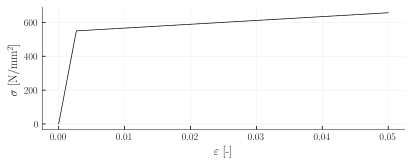
\includegraphics{index_files/mediabag/05_Versuchsnachrechnung_VM1_files/figure-pdf/fig-sigma-epsilon-sv14-output-1.pdf}

}

\caption{\label{fig-sigma-epsilon-sv14}Spannungs-Dehnungs-Beziehung der
Schubbewehrung, übernommen aus
{[}\citeproc{ref-gitz_ansatze_2024}{1}{]}}

\end{figure}%

Wird das Spannungs-Dehnungs-Verhalten gemäss der
Abbildung~\ref{fig-sigma-epsilon-sv14} berücksichtigt. So resultiert mit
der Querschnittsfläche der Schubbewehrung pro Spannungsfeld die
entsprechende Kraftkomponente der Wegfedercharakteristik. Die
Verformungskomponente entspricht der Dehnung multipliziert mit dem
Hebelarm der inneren Kräfte. Dies führt zum Kraft-Verformungs-Verhalten
für ein Spannungsfeld. Um die Wegfedercharakteristik einer einzelnen
Feder zu erhalten, ist die Verformung um die Anzahl an Stabelementen im
Spannungsfeld zu reduzieren. Der Reduktionsfaktor zur Erhöhung der
Steifigkeit der Feder folgt zu:

$$
\begin{aligned}
\gamma_{E_{_{}}} &= z_{_{}} \cdot \frac{ 1 }{ \tan \left( \theta_{c3_{_{}}} \right) } \cdot \frac{1} { l_{E} } \; 
\end{aligned}
$$

$$
\begin{aligned}
\gamma_{E_{_{}}} &= 75\ \;
\end{aligned}
$$

Die Abbildung~\ref{fig-wegfeder-schub-sv14} zeigt das
Kraft-Verformungs-Verhalten für die Federn des Stabmodells in vertikaler
Richtung. Das Verhalten ist analog dem des bilinearen
Spannungs-Dehnungs-Diagramms.

\begin{figure}[H]

\centering{

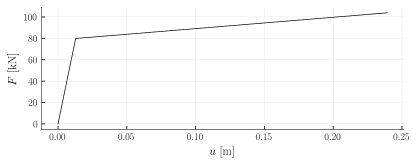
\includegraphics{index_files/mediabag/05_Versuchsnachrechnung_VM1_files/figure-pdf/fig-wegfeder-schub-sv14-output-1.pdf}

}

\caption{\label{fig-wegfeder-schub-sv14}Berechnete
Wegfedercharakteristik der Federn des Vierpunktbiegeversuches}

\end{figure}%

\subsection{Modellergebnisse}\label{modellergebnisse-1}

Mit den bestimmten Federcharakteristiken kann die Biegelinie des Systems
ermittelt werden unter Berücksichtigung der Schub- und Biegeverformungen
basierend auf nichtlinearen Stoffgesetzen. Die
Abbildung~\ref{fig-l-w-sv14} zeigt das Last-Verformungs-Diagramm des
Systems am Punkt \(w_1\). Der Verformungsverlauf zeigt Abweichungen zu
den gemessenen Resultaten.

\begin{figure}[H]

\centering{

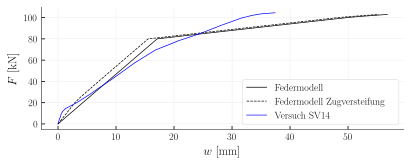
\includegraphics{index_files/mediabag/05_Versuchsnachrechnung_VM1_files/figure-pdf/fig-l-w-sv14-output-1.pdf}

}

\caption{\label{fig-l-w-sv14}Last-Verformungs-Verlauf am Punkt \(w_1\)
aus dem Federmodell und aus den Versuchsmessungen}

\end{figure}%

Bis zum Erreichen des ersten Knicks im Verlauf des Federmodells ist das
Modell etwas zu steif. Trotzdem ist dies akzeptabel. Das zu steife
Verhalten lässt sich auf die Vernachlässigung der Stauchung der
Druckdiagonalen und der Gurtdehnung zurückführen. In der
Abbildung~\ref{fig-schubverf_sigrist} ist ein Modell zur Ermittlung der
Schiebung am Fachwerk gezeigt. Dies bietet einen Ansatz zur erweiterten
Bestimmung der Schubsteifigkeit. Der Knick resultiert aus dem Fliessen
der Schubbewehrung. Bei den Versuchsresultaten ist bei gleicher
Verformung ebenfalls ein Knick zu erkennen. Jedoch ist das Lastniveau
nicht deckungsgleich.

\begin{figure}[H]

\centering{

\includegraphics{index_files/mediabag/../imgs/schubverformungen_sigrist.pdf}

}

\caption{\label{fig-schubverf_sigrist}Ermittlung der Schiebung am
Fachwerk, a) Dehnung der Bügel b) Stauchung der Diagonalen c) mittlere
Gurtdehnung, nach {[}\citeproc{ref-sigrist_zum_1995}{4}{]}}

\end{figure}%

Das darauffolgende verfestigende Verhalten weicht deutlich von dem
Versuchsverhalten ab. Des Weiteren hat die Berechnung im Modell ein
Schubversagen prognostiziert. Die Versuchsdaten beschreiben ein
Biegeversagen im Feld. Das Modell beschreibt das Versuchsverhalten
mangelhaft. Dies ist den Unschärfen der Stoffgesetze zuzuschreiben.

Abschliessend wird der, aus dem Modell exportierte, Verdrehungsverlauf
aufgezeigt. Sowie wird der daraus berechnete Krümmungsverlauf
aufgezeigt.

\begin{figure}[H]

\centering{

\includegraphics{index_files/mediabag/05_Versuchsnachrechnung_VM1_files/figure-pdf/fig-phi-max-sv14-output-1.pdf}

}

\caption{\label{fig-phi-max-sv14}Verdrehungsverlauf aus dem Federmodell
für die Höchstlast des Vierpunktbiegeversuchs}

\end{figure}%

Der Krümmungsverlauf gibt Aufschluss über den Biegesteifigkeitenverlauf
entlang der Stabachse. Die Darstellung weist Unreinheiten auf. Der grobe
Verlauf ist jedoch erkennbar. Es zeigt sich, dass die Längsbewehrung in
Feldmitte zu fliessen beginnt.

\begin{figure}[H]

\centering{

\includegraphics{index_files/mediabag/05_Versuchsnachrechnung_VM1_files/figure-pdf/fig-chi-max-sv14-output-1.pdf}

}

\caption{\label{fig-chi-max-sv14}Berechneter Krümmungsverlauf aus dem
Verdrehungsverlauf für den Vierpunktbiegeversuch}

\end{figure}%

Obwohl der Verformungsverlauf mangelhaft beschrieben wird, deckt sich
das Verhalten des Federmodells mit den Berechnungen der Vorarbeit. Die
Modellverifizierung wird somit als gelungen betrachtet.

\bookmarksetup{startatroot}

\chapter{Modellanwendung - vorgespannter
Träger}\label{modellanwendung---vorgespannter-truxe4ger}

Nachdem das Kapitel~\ref{sec-verifizierung} die Anwendbarkeit des
Modells bestätigt hat, wird in diesem Kapitel ein Versuch eines
vorgespannten Trägers mittels dem Federmodell nachgerechnet. Der
Versuchsbeschrieb liefert die nötigen Grundlagen. Es wird die Bestimmung
der Momenten-Krümmungs-Beziehung aufgezeigt. Auf das Versatzmass und auf
die Schubverformungen wird nicht eingegangen. Abschliessend werden die
Versuchsresultate mit den berechneten Grössen verglichen und
kommentiert. Zudem wird die Compatible Stress Field Method (CSFM)
mittels der Software IDEAStatiCa angewendet und mit dem Federmodell
verglichen.

\section{Versuchsbeschrieb}\label{versuchsbeschrieb-2}

Der vorgespannte Träger T6 wurde aus dem Versuchsbericht
{[}\citeproc{ref-sigrist_versuche_1993}{5}{]} entnommen. Es handelt sich
um einen einfachen Balken mit einer Auskragung. Die Geometrie des
Versuchs in Längsrichtung ist in Abbildung~\ref{fig-geometrie_t6}
gezeigt.

\begin{figure}[H]

\centering{

\includegraphics{index_files/mediabag/../imgs/T6_geometrie_laengs.pdf}

}

\caption{\label{fig-geometrie_t6}Geometrie des Versuchsträgers T6,
entnommen aus {[}\citeproc{ref-sigrist_versuche_1993}{5}{]}}

\end{figure}%

Der Querschnitt des Trägers ist in Abbildung~\ref{fig-geometrie_qs_t6}
gezeigt. Versehen ist das I-Profil mit den Abmessungen. Der Steg ist am
Stabende und Anfang verbreitert.

\begin{figure}[H]

\centering{

\includegraphics{index_files/mediabag/../imgs/T6_geometrie_qs.pdf}

}

\caption{\label{fig-geometrie_qs_t6}Geometrie des Querschnitts des
Versuchsträgers T6, entnommen aus
{[}\citeproc{ref-sigrist_versuche_1993}{5}{]}}

\end{figure}%

Das Bewehrungslayout im Querschnitt zeigt die
Abbildung~\ref{fig-bewehrung_qs_t6}. Die Bewehrungsüberdeckung beträgt
in allen Richtungen \(20\) mm. Mit Grossbuchstaben \(A\) bis \(I\) sind
die Bewehrungslagen in längsrichtung beschrieben. Die Schubbügel sind
mit den Kleinbuchstaben \(i\) bis \(iii\) bezeichnet.

\begin{figure}[H]

\centering{

\includegraphics{index_files/mediabag/../imgs/T6_bewehrung_qs.pdf}

}

\caption{\label{fig-bewehrung_qs_t6}Bewehrungslayout im Querschnitt des
Versuchsträgers T6, entnommen aus
{[}\citeproc{ref-sigrist_versuche_1993}{5}{]}}

\end{figure}%

Die verlegte schlaffe Bewehrung ist in der
Abbildung~\ref{fig-bewehrung_laengs_t6} gezeigt. Diese ist an mehreren
Punkten abgestuft. Die Stosslänge beträgt jeweils \(60\) cm.

\begin{figure}[H]

\centering{

\includegraphics{index_files/mediabag/../imgs/T6_bewehrung_laengs.pdf}

}

\caption{\label{fig-bewehrung_laengs_t6}Bewehrungslayout in
Längsrichtung des Versuchsträgers T6, entnommen aus
{[}\citeproc{ref-sigrist_versuche_1993}{5}{]}}

\end{figure}%

Die Position der Vorspannung ist in der
Abbildung~\ref{fig-vorspannung_t6} gezeigt. Das Kabel konnte im Mittel
bis auf \(730\) kN vorgespannt werden. Das Spannkabel besteht aus 4
Litzen mit Durchmesser \(0.6''\). Eingelegt sind diese in einem
Stahlhüllrohr, welches nachträglich ausinjiziert wurde.

\begin{figure}[H]

\centering{

\includegraphics{index_files/mediabag/../imgs/T6_vorspannung_laengs.pdf}

}

\caption{\label{fig-vorspannung_t6}Vorspannungslayout des
Versuchsträgers T6. Horizontaler Abstand {[}m{]} und vertikale Position
{[}mm{]}, gemessen von der Unterkante des Trägers, entnommen aus
{[}\citeproc{ref-sigrist_versuche_1993}{5}{]}}

\end{figure}%

Die Lastsituation zeigt die Abbildung~\ref{fig-last_t6}. Am Ende des
Kragarms greift eine Einzellast \(P\) an. Mit \(Q\) wird eine
Streckenlast simuliert. Der Träger ist an den Punkten \(A\) und \(B\)
gelenkig gelagert. Zusätzlich ist der Träger beim Auflager \(B\)
horizontal gehalten.

\begin{figure}[H]

\centering{

\includegraphics{index_files/mediabag/../imgs/T6_last_laengs.pdf}

}

\caption{\label{fig-last_t6}Lagerung und Position der Pressenkräfte des
Versuchsträgers T6, entnommen aus
{[}\citeproc{ref-sigrist_versuche_1993}{5}{]}}

\end{figure}%

\subsection{Berechnungsgrössen}\label{berechnungsgruxf6ssen}

In diesem Abschnitt werden die allgemein verwendeten Parameter
aufgelistet. Gegliedert nach den einzelnen Aspekten des Versuchs.
Aufgezeigt sind sämtliche Baustoffkennwerte. Dazu sind die geometrischen
Grössen erwähnt.

\subsubsection{Vorspannung}\label{vorspannung}

Der folgende Abschnitt charakterisiert die Vorspannung. Aufgezeigt ist
die mittlere initiale Vorspannkraft, die Fliessgrenze der Litzen, sowie
deren Zugfestigkeit und entsprechende Bruchdehnung. Ebenfalls
dargestellt ist der Elastizitätsmodul, die Querschnittsfläche des
Spannglieds und der angewendete Verlustfaktor. Die aus den Proben
bestimmte Materialkennlinien sind in der
Abbildung~\ref{fig-sigma_eps_spannstahl} gezeigt.

\begin{figure}[H]

\centering{

\includegraphics{index_files/mediabag/../imgs/t6_spannstahl.pdf}

}

\caption{\label{fig-sigma_eps_spannstahl}Spannungs-Dehnungs-Diagramm und
Kraft-Verformungs-Diagramm des Spannstahls mittels Zugproben ermittelt,
entnommen aus {[}\citeproc{ref-sigrist_versuche_1993}{5}{]}}

\end{figure}%

$$
\begin{aligned}
f_{py} &= 1706.0\ \frac{\mathrm{N}}{\mathrm{mm}^{2}} \; 
 &f_{pu} &= 1855.0\ \frac{\mathrm{N}}{\mathrm{mm}^{2}} \; 
 &V_{om} &= 730.0\ \mathrm{kN} \; 
\\[10pt]
 A_{p} &= 596.0\ \mathrm{mm}^{2} \; 
 &E_{p} &= 190000.0\ \frac{\mathrm{N}}{\mathrm{mm}^{2}} \; 
 &\varepsilon_{pu} &= 1.5\ \mathrm{\%} \; 
\\[10pt]
 \eta &= 0.9 \; \;\textrm{(Verlustfaktor)}
\end{aligned}
$$

Der Verlustfaktor wird ohne Berücksichtigung von Langzeiteffekten auf
90\% geschätzt. Daraus resultiert die Vorspannkraft zu:

$$
\begin{aligned}
P_{\infty} &= \eta \cdot V_{om} \; 
\end{aligned}
$$

$$
\begin{aligned}
P_{\infty} &= 657.0\ \mathrm{kN} \;
\end{aligned}
$$

Die Spannung im Spannglied aufgrund der Vorspannung definiert sich zu:

$$
\begin{aligned}
\sigma_{P_{\infty}} &= \frac{ P_{\infty} }{ A_{p} } \; 
\end{aligned}
$$

$$
\begin{aligned}
\sigma_{P_{\infty}} &= 1102.3\ \frac{\mathrm{N}}{\mathrm{mm}^{2}} \;
\end{aligned}
$$

\subsubsection{Beton}\label{beton}

Die Parameter sind Mittelwerte aus Betonwürfel- und Betonzylinderproben,
entnommen aus dem Versuchsbericht
{[}\citeproc{ref-sigrist_versuche_1993}{5}{]}. In der
Abbildung~\ref{fig-sigma_eps_beton} ist das Spannungs-Dehnungs-Verhalten
der Betonproben für die gesamte Versuchsserie aufgezeigt.

\begin{figure}[H]

\centering{

\includegraphics{index_files/mediabag/../imgs/t6_beton.pdf}

}

\caption{\label{fig-sigma_eps_beton}Spannungs-Dehnungs-Diagramm des
Betons, dargestellt sind diese für die Versuchskörper \(T_1\) bis
\(T_6\), entnommen aus {[}\citeproc{ref-sigrist_versuche_1993}{5}{]}}

\end{figure}%

Dabei beschreibt \(f_c\) die maximale Druckfestigkeit. Die Zugfestigkeit
wird dabei mit \(f_{ct}\) bezeichnet. Der Elasitzitätsmodul \(E_c\), die
Dichte \(\rho_c\) und die Bruchstauchung \(\varepsilon_{cu}\) schliessen
den Beschrieb ab.

$$
\begin{aligned}
f_{c} &= 52.10\ \frac{\mathrm{N}}{\mathrm{mm}^{2}} \; 
 &f_{ct} &= 4.30\ \frac{\mathrm{N}}{\mathrm{mm}^{2}} \; 
 &E_{c} &= 50200.00\ \frac{\mathrm{N}}{\mathrm{mm}^{2}} \; 
\\[10pt]
 \rho_{c} &= 2409.00\ \frac{\mathrm{kg}}{\mathrm{m}^{3}} \; 
 &\varepsilon_{cu} &= 0.35\ \mathrm{\%} \;
\end{aligned}
$$

\subsubsection{Betonstahl}\label{betonstahl}

Die dargestellten Parameter sind Mittelwerte aus den durchgeführten
Zugproben am Betonstahl. Diese sind ebenfalls aus dem Versuchsbericht
{[}\citeproc{ref-sigrist_versuche_1993}{5}{]} entnommen worden.

\begin{figure}[H]

\centering{

\includegraphics{index_files/mediabag/../imgs/t6_betonstahl.pdf}

}

\caption{\label{fig-sigma_eps_betonstahl}Spannungs-Dehnungs-Diagramm und
Kraft-Verformungs-Diagramm mittels Zugproben ermittelt für den
Betonstahl, entnommen aus {[}\citeproc{ref-sigrist_versuche_1993}{5}{]}}

\end{figure}%

Die Abbildung~\ref{fig-sigma_eps_betonstahl} zeigt das
Spannungs-Dehnungs-Verhalten, sowie das Kraft-Verformungs-Verhalten der
Probe eines Durchmessers \(16\) mm Stabs. Im Spannungs-Dehnungs-Diagramm
ist lediglich das Fliessplateau dargestellt. Dabei beschreibt \(f_{sy}\)
die Fliessgrenze, \(f_{su}\) die Zugfestigkeit. \(\varepsilon_{su}\)
bezeichnet die Bruchdehnung und \(E_s\) den Elastizitätsmodul.

$$
\begin{aligned}
f_{sy} &= 500.0\ \mathrm{MPa} \; 
 &f_{su} &= 630.0\ \mathrm{MPa} \; 
 &\varepsilon_{su} &= 12.7\ \mathrm{\%} \; 
\\[10pt]
 E_{s} &= 205000.0\ \frac{\mathrm{N}}{\mathrm{mm}^{2}} \;
\end{aligned}
$$

\subsubsection{Geometrie}\label{geometrie}

Die Parameter der Geometrie des Querschnitts beziehen sich auf die
Abbildung~\ref{fig-geometrie_qs_t6}. Der Schwerpunkt \(S_z\) des
Querschnitts ist von der Unterkante aus gemessen.

$$
\begin{aligned}
h_{sup} &= 140.0\ \mathrm{mm} \; 
 &h_{inf} &= 180.0\ \mathrm{mm} \; 
 &h &= 800.0\ \mathrm{mm} \; 
\\[10pt]
 b_{inf} &= 400.0\ \mathrm{mm} \; 
 &b_{sup} &= 800.0\ \mathrm{mm} \; 
 &S_{z} &= 459.5\ \mathrm{mm} \; 
\\[10pt]
 L &= 13600.0\ \mathrm{mm} \;
\end{aligned}
$$

\subsection{Versuchsergebnisse}\label{versuchsergebnisse-2}

Der Versuchsbeschrieb wird mit den gemessenen Resultaten abgeschlossen.
Gemessen wurde der Einfluss der Vorspannung beim Einbringen des Trägers,
sowie das Verhalten unter Belastung mittels Pressenkräften. Die
Abbildung~\ref{fig-durchbiegung_laengs_t6} zeigt den Verformungsverlauf
für den gesamten Träger in Abhängigkeit der Laststufen.

\begin{figure}[H]

\centering{

\includegraphics{index_files/mediabag/../imgs/T6_durchbiegung_laengs.pdf}

}

\caption{\label{fig-durchbiegung_laengs_t6}Verformungsverlauf des
Versuchsträgers T6, entnommen aus
{[}\citeproc{ref-sigrist_versuche_1993}{5}{]}}

\end{figure}%

Die Abbildung~\ref{fig-durchbiegung_t6} zeigt oben links das
Kraft-Verformungs-Diagramm für die Einzellast \(P\) mit der gemessenen
Verformung \(w_{10}\) an der Stelle \(10\), gemäss der
Abbildung~\ref{fig-messstellen_t6}. Oben rechts ist das
Kraft-Verformungs-Diagramm für die simulierte Streckenlast \(Q\) und die
Verformung \(w_{18}\) aufgezeigt.

\begin{figure}[H]

\centering{

\includegraphics{index_files/mediabag/../imgs/t6_messstellen.pdf}

}

\caption{\label{fig-messstellen_t6}Messstellen des Versuchsträgers T6,
entnommen aus {[}\citeproc{ref-sigrist_versuche_1993}{5}{]}}

\end{figure}%

Das Diagramm unten links gibt Aufschluss über den Belastungshergang.
Zunächst wurde die Einzellast \(P\) gesteigert bis ca. \(480\) kN. Ab
dieser Stufe verblieb die Einzellast in etwa auf diesem Niveau, die
Streckenlast \(Q\) wurde abschliessend erhöht, bis der Träger versagte.
Das Versagen geschah schlagartig, durch das Versagen der Vorspannlitzen
links neben dem Auflager \(B\). Der Versuch wurde weggesteuert gefahren.

\begin{figure}[H]

\centering{

\includegraphics{index_files/mediabag/../imgs/T6_durchbiegungen.pdf}

}

\caption{\label{fig-durchbiegung_t6}Last-Verformungs-Verhalten des
Versuchsträgers T6, entnommen aus
{[}\citeproc{ref-sigrist_versuche_1993}{5}{]}}

\end{figure}%

\section{Modellierung}\label{modellierung-2}

Basierend auf dem Versuchsbeschrieb wird in diesem Abschnitt auf die
Modellierung eingegangen. Der Versuch wird mittels dem Federmodell
modelliert. Das statische System dazu ist in der
Abbildung~\ref{fig-system_t6} aufgezeigt.

\begin{figure}[H]

\centering{

\includegraphics{index_files/mediabag/../imgs/T6_system.pdf}

}

\caption{\label{fig-system_t6}Statisches System des Versuchs \(T_6\)}

\end{figure}%

Die Auflagerbreiten sind vernachlässigt. Auf die Darstellung der Federn
wird verzichtet. Diese sind in einem Abstand von \(l_E\) angeordnet.

$$
\begin{aligned}
l_{E} &= 10.0\ \mathrm{cm} \; \;\textrm{(Elementlänge des biege- und schubsteifen Stabs)}
\end{aligned}
$$

Die Elementlänge wird im Vergleich mit den Versuchen aus dem
Kapitel~\ref{sec-verifizierung} deutlich grösser gewählt. Dies ist auf
die aufwändige Bestimmung der Momenten-Krümmungs-Beziehung
zurückzuführen.

\subsection{Lastfälle}\label{lastfuxe4lle}

Die unterschiedliche Belastungsgeschwindigkeit liefert eine gewisse
Komplexität bei der Modellierung. Sowie wird die Vorspannung als
Einwirkung interpretiert. Abschliessend ist aufgrund der Vorspannung das
Eigengewicht zu berücksichtigen, da dies den negativ gerichteten
Umlenkkräften entgegenwirkt. Es wird zwischen den Lastfällen
Eigengewicht, Vorspannung und den Pressenkräften unterschieden. Diese
werden folgend beschrieben:

\subsubsection{Eigengewicht}\label{eigengewicht}

Das Eigengewicht wird als Streckenlast auf dem gesamten statischen
System angeordnet. Ermittelt aus der Betonquerschnittsfläche und
entsprechender Dichte.

\begin{figure}[H]

\centering{

\includegraphics{index_files/mediabag/../imgs/T6_eigengewicht_lf.pdf}

}

\caption{\label{fig-t6_lastfall_eg}Statisches System mit Streckenlast
durch Eigengewicht}

\end{figure}%

Dabei beträgt die Querschnittsfläche des I-Profils:

$$
\begin{aligned}
A_{c} &= 302800.0\ \mathrm{mm}^{2} \;
\end{aligned}
$$

Welche zu folgendem Eigengewicht führt:

$$
\begin{aligned}
g_{c} &= A_{c} \cdot \rho_{c} \cdot 10 \cdot \frac{ m }{ \left( s \right) ^{ 2 } } \; 
\end{aligned}
$$

$$
\begin{aligned}
g_{c} &= 7.3\ \frac{\mathrm{kN}}{\mathrm{m}} \;
\end{aligned}
$$

\subsubsection{Vorspannung}\label{vorspannung-1}

Unabhängig von der Versuchslast gilt es den Einfluss der Vorspannung zu
modellieren. Dazu wird die Vorspannung als Anker - Umlenk - und
Reibungskräfte (AUR) interpretiert. Grundlagen dazu sind in
{[}\citeproc{ref-thoma_vorspannung_2020}{6}{]} aufgezeigt. Die
Interpretation nach AUR führt zu Umlenkkräften im parabolischen Bereich
der Vorspannung, sowie zu Normal- und Querkräften, und einem Biegemoment
bei der Verankerungsstelle. Aufgezeigt ist der Lastfall in der
Abbildung~\ref{fig-t6_lastfall_p}.

\begin{figure}[H]

\centering{

\includegraphics{index_files/mediabag/../imgs/T6_vorspann_lf.pdf}

}

\caption{\label{fig-t6_lastfall_p}Statisches System mit Anker und
Umlenkkräften, die Einwirkungen sind in der entsprechenden
Wirkungsrichtung dargestellt}

\end{figure}%

Zur Quantifizierung der Einwirkung wird in einem ersten Schritt die
Kabelgeometrie, sprich \(z_p(x)\) analytisch beschrieben. Dargestellt
ist die Funktion in der Abbildung~\ref{fig-z_p_von_x}. Zusätzlich ist
der Umriss des Trägers dargestellt.

\begin{figure}[H]

\centering{

\includegraphics{index_files/mediabag/06_Vorspannversuch_files/figure-pdf/fig-z_p_von_x-output-1.pdf}

}

\caption{\label{fig-z_p_von_x}Geometrie des Spannkabels als Funktion
\(z_p(x)\)}

\end{figure}%

Unter Berücksichtigung der folgenden Gleichung können die Umlenkkräfte
bestimmt werden.

\[
u_p(x) \simeq z_p(x)'' \cdot P_{\infty}
\]

Diese betragen dabei:

$$
\begin{aligned}
u_{P1} &= 115.6\ \frac{\mathrm{kN}}{\mathrm{m}} \; 
 &u_{P2} &= -34.3\ \frac{\mathrm{kN}}{\mathrm{m}} \;
\end{aligned}
$$

Darauffolgend wird die Spannstelle betrachtet. Die Exzentrizität des
Spannkabels zum geometrischen Schwerpunkt des Querschnitts führt zu
einem Biegemoment. Die Exzentrizität entspricht dabei:

$$
\begin{aligned}
e_{P0} &= 55.5\ \mathrm{mm} \; \;\textrm{($x=0$)}
 &e_{P1} &= -65.3\ \mathrm{mm} \; \;\textrm{($x=L$)}
\end{aligned}
$$

Multipliziert mit der Vorspannkraft folgt das Biegemoment bei der
Spannstelle links zu:

$$
\begin{aligned}
M_{P0} &= P_{\infty} \cdot e_{P0} \; 
\end{aligned}
$$

$$
\begin{aligned}
M_{P0} &= 36.5\ \mathrm{kN} \cdot \mathrm{m} \; \;\textrm{(OK Zug)}
\end{aligned}
$$

Und bei der Spannstelle rechts zu:

$$
\begin{aligned}
M_{P1} &= P_{\infty} \cdot e_{P1} \; 
\end{aligned}
$$

$$
\begin{aligned}
M_{P1} &= -42.9\ \mathrm{kN} \cdot \mathrm{m} \; \;\textrm{(UK Zug)}
\end{aligned}
$$

Die Vertikalkomponente der Spannkraft resultiert aus der Transformation
der Normalkraft mittels der Neigung des Spannkabels bei der Spannstelle.
Diese entspricht beim Trägeranfang:

$$
\begin{aligned}
P_{V0} &= \sin \left( \alpha_{0} \right) \cdot P_{\infty}  = \sin \left( 0.1 \right) \cdot 657.0\ \mathrm{kN} &= 73.1\ \mathrm{kN}  
\end{aligned}
$$

Und beim Trägerende entspricht die vertikale Kraft:

$$
\begin{aligned}
P_{V1} &= \sin \left( \alpha_{1} \right) \cdot P_{\infty}  = \sin \left( 0.2 \right) \cdot 657.0\ \mathrm{kN} &= 98.7\ \mathrm{kN}  
\end{aligned}
$$

\subsubsection{Pressenkräfte}\label{pressenkruxe4fte}

\begin{figure}[H]

\centering{

\includegraphics{index_files/mediabag/../imgs/T6_versuch_lf.pdf}

}

\caption{\label{fig-t6_lastfall_versuch}Statisches System mit der
Laststellung aus den Pressen}

\end{figure}%

Gemäss dem Versuchsbeschrieb lässt sich der Träger bis zu den folgenden
maximalen Lasten belasten:

$$
\begin{aligned}
Q_{max} &= 1638.0\ \mathrm{kN} \; 
 &P_{max} &= 512.0\ \mathrm{kN} \; 
 &L_{q} &= 9.0\ \mathrm{m} \; 
\\[10pt]
\end{aligned}
$$

Die mit \(Q\) simulierte Streckenlast wird als effektive Streckenlast
modelliert. Dies führt zu folgender Grösse:

$$
\begin{aligned}
q_{Q_{max}} &= \frac{ Q_{max} }{ L_{q} }  = \frac{ 1638.0\ \mathrm{kN} }{ 9.0\ \mathrm{m} } &= 182.0\ \frac{\mathrm{kN}}{\mathrm{m}}  
\end{aligned}
$$

Im Stabstatikmodell werden zwei Lastfälle definiert zum Abbilden der
Pressenkräfte. Zum einen wird die Einzellast \(P_{1}\) und die
entsprechende Streckenlast \(q_{1}\) angesetzt. Betitelt wird diese
Lastsituation mit \emph{Pressenkräfte 1}. Betragsmässig entspricht der
Lastfall \emph{Pressenkräfte 1} in etwa der Laststufe 8 gemäss der
Abbildung~\ref{fig-durchbiegung_t6}. Bei der Berechnung werden \(P_1\)
und \(q_1\) inkrementell gesteigert. Sie liefern somit Resultate für
sämtliche Laststufen unterhalb der Laststufe 8.

$$
\begin{aligned}
P_{1} &= 475.0\ \mathrm{kN} \; 
 &q_{1} &= 80.0\ \frac{\mathrm{kN}}{\mathrm{m}} \; 
 &Q_{1} &= 720.0\ \mathrm{kN} \; 
\\[10pt]
\end{aligned}
$$

Der zweite Lastfall beinhaltet die Einzellast \(P_{1}\), sowie die
Streckenlast \(q_1\) des Lastfalls \emph{Pressenkräfte \(1\)}. Ergänzend
wird eine Einzellast \(P_{\Delta}\) und eine Streckenlast \(q_{\Delta}\)
an den gleichen Positionen eingeführt. Diese werden inkrementell
gesteigert, die Lasten des Lastfalls \emph{Pressenkräfte \(1\)} bleiben
konstant. Die Lasten wurden iterativ bestimmt und entsprechen der
Traglast des Modells. Der Lastfall wird mit \emph{Pressenkräfte \(2\)}
bezeichnet.

$$
\begin{aligned}
P_{\Delta} &= 11.0\ \mathrm{kN} \; 
 &q_{\Delta} &= 90.0\ \frac{\mathrm{kN}}{\mathrm{m}} \; 
 &P_{2} &= 486.0\ \mathrm{kN} \; 
\\[10pt]
 q_{2} &= 169.9\ \frac{\mathrm{kN}}{\mathrm{m}} \; 
 &Q_{2} &= 1529.5\ \mathrm{kN} \;
\end{aligned}
$$

Es zeigen sich Differenzen zwischen der gemessenen Traglast und der
Traglast des Modells.

\subsection{Baustoffe}\label{baustoffe}

Folgend wird die Modellierung der Stoffgesetze beschrieben. Diese dienen
lediglich zur Bestimmung der Momenten-Krümmungs-Beziehung. Der Beton
wird mit der Parabel nach Eurocode 2 bzw. DIN 1045 zur nichtlinearen
Schnittgrössenermittlung beschrieben. Dabei wird die Würfelfestigkeit
als Bauteilfestigkeit angesetzt.

\begin{figure}[H]

\centering{

\includegraphics{index_files/mediabag/06_Vorspannversuch_files/figure-pdf/fig-sigma_epc_t6-output-1.pdf}

}

\caption{\label{fig-sigma_epc_t6}Modelliertes
Spannungs-Dehnungs-Verhalten des Betons des Versuchsträgers T6, mit
ergänzten Versuchsmessungen}

\end{figure}%

Das Verhalten der schlaffen Bewehrung wird mit einem bilinearen
Stoffgesetzt modelliert. Aufgezeigt ist das Verhalten in der
Abbildung~\ref{fig-sigma_eps_t6}

\begin{figure}[H]

\centering{

\includegraphics{index_files/mediabag/06_Vorspannversuch_files/figure-pdf/fig-sigma_eps_t6-output-1.pdf}

}

\caption{\label{fig-sigma_eps_t6}Modelliertes
Spannungs-Dehnungs-Verhalten des Betonstahls des Versuchsträgers T6, mit
ergänzten Versuchsmessungen}

\end{figure}%

Abgeschlossen wird die Modellierung der Baustoffe mit der
Spannungs-Dehnungs-Beziehung der Vorspannlitzen. Betrachtet man das
Spannungs-Dehnungs-Verhalten des Spannstahls, so ist ersichtlich, dass
durch die Vorspannkraft die Spannlitzen noch nicht vollständig
ausgeschöpft sind. Die Differenz bis zur Zugfestigkeit kann mittels
Biegung aktiviert werden und wird bei der Querschnittsanalyse
mitberücksichtigt. Dargestellt ist Ausnutzung der Vorspannkraft in der
Abbildung~\ref{fig-ausnutzung_sigma_p}.

\begin{figure}[H]

\centering{

\includegraphics{index_files/mediabag/06_Vorspannversuch_files/figure-pdf/fig-ausnutzung_sigma_p-output-1.pdf}

}

\caption{\label{fig-ausnutzung_sigma_p}Spannungs-Dehnungs-Beziehung der
Spannlitzen mit ergänzter Ausnutzung durch die Vorspannkraft}

\end{figure}%

Dies führt zu der Spannungs-Dehnungs-Beziehung in der
Abbildung~\ref{fig-sigma_eps_vorspannung_t6}. Dargestellt ist lediglich
der positive Spannungsbereich. Im negativen Spannungsbereich wird ein
linear-elastisches Verhalten vorausgesetzt. Dies ist jedoch nicht
relevant, da die Vorspannung lediglich Zugbeanspruchungen erfährt.

\begin{figure}[H]

\centering{

\includegraphics{index_files/mediabag/06_Vorspannversuch_files/figure-pdf/fig-sigma_eps_vorspannung_t6-output-1.pdf}

}

\caption{\label{fig-sigma_eps_vorspannung_t6}Modelliertes
Spannungs-Dehnungs-Verhalten der Vorspannung des Versuchsträgers T6, mit
ergänzten Versuchsmessungen}

\end{figure}%

\subsection{Momenten-Krümmungs-Beziehung}\label{momenten-kruxfcmmungs-beziehung}

Basierend auf den eben beschriebenen Materialgesetzen wird die
Momenten-Krümmungs-Beziehung ermittelt. Die Ermittlung zeigt bei diesem
Versuch eine gewisse Komplexität. Grundsätzlich gilt es für jede
Abstufung der Bewehrung eine separate Momenten-Krümmungs-Beziehung
herzuleiten.

Durch die Berücksichtigung der Vorspannung und deren parabolischen
Geometrie gilt es die Momenten-Krümmungs-Beziehung unter Variation der
Spannkabellage zu definieren, was die Komplexität der
Momenten-Krümmungs-Beziehung zusätzlich erhöht. Die numerische
Bestimmung wird mit einer Querschnittsanalyse-Software durchgeführt. Es
werden 136 Querschnitte im Abstand der Elementlänge \(l_E\) entlang des
Stabs analysiert, gezeigt sind diese im Anhang.

\subsubsection{Verifizierung}\label{verifizierung}

Um die Resultate der Querschnittsanalyse-Software zu verifizieren, wird
hier eine Abschätzung aufgezeigt. Die Krümmung und das Biegemoment wird
für den Querschnitt bei \(x=3.5\)m abgeschätzt. Die Bewehrungsführung
wird dabei vereinfacht, schematisch ist dies für negative Biegung
gezeigt in der Abbildung~\ref{fig-t6_qs_approx}.

\begin{figure}[H]

\centering{

\includegraphics{index_files/mediabag/../imgs/T6_qs_approx.pdf}

}

\caption{\label{fig-t6_qs_approx}Vereinfachung der Bewehrungsführung,
Druckbewehrung vernachlässigt, Zugbewehrung zu einem Stab
zusammengefasst}

\end{figure}%

Dabei werden vier Zustände betrachtet. Das Fliessen der Vorspannung bei
negativer Biegung, sowie wird der negative Biegewiderstand ermittelt.
Das Fliessen der schlaffen Bewehrung bei positiver Biegung wird
betrachtet, und abschliessend wird der positive Biegewiderstand
berechnet.

\paragraph{Fliessen der Vorspannung - Zug im Obergurt
(1)}\label{fliessen-der-vorspannung---zug-im-obergurt-1}

Im Zustand \(1\) wird vorausgesetzt, dass die Vorspannlitzen die
Fliessgrenze erreichen. Die schlaffe Bewehrung hat ebenfalls die
Fliessgrenze erreicht. Die Spannungsverteilung des Betons wird als
Dreiecksverlauf angenommen. Der Beton erreicht die Druckfestigkeit.

\begin{figure}[H]

\centering{

\includegraphics{index_files/mediabag/../imgs/T6_qs_My_pos.pdf}

}

\caption{\label{fig-t6_qs_My_pos}Querschnittsanalyse bei \(x=3.5\) m
entlang der Stabachse, Vorspannung erreicht Fliessgrenze, Beton erreicht
Druckfestigkeit}

\end{figure}%

Die Querschnittsfläche der schlaffen Bewehrung beträgt dabei:

$$
\begin{aligned}
A_{s1} &= \left( 4 \cdot \frac{ \left( 14 \cdot \mathrm{mm} \right) ^{ 2 } }{ 4 } + 12 \cdot \frac{ \left( 12 \cdot \mathrm{mm} \right) ^{ 2 } }{ 4 } \right) \cdot \pi \; 
\end{aligned}
$$

$$
\begin{aligned}
A_{s1} &= 1972.9\ \mathrm{mm}^{2} \;
\end{aligned}
$$

Die statische Höhe wird abgeschätzt und beträgt:

$$
\begin{aligned}
d_{1} &= h - \frac{ h_{sup} }{ 2 } \; 
\end{aligned}
$$

$$
\begin{aligned}
d_{1} &= 730.0\ \mathrm{mm} \;
\end{aligned}
$$

Mittels horizontalen Gleichgewichts der Kräfte lässt sich die
Druckzonenhöhe bestimmen:

$$
\begin{aligned}
x_{1} &= \frac{ A_{s1} \cdot f_{sy} + A_{p} \cdot \left( f_{py} - \sigma_{P_{\infty}} \right) + P_{\infty} }{ b_{inf} \cdot 0.5 \cdot f_{c} } \; 
\end{aligned}
$$

$$
\begin{aligned}
x_{1} &= 192.2\ \mathrm{mm} \;
\end{aligned}
$$

Mit welcher das Fliessmoment ermittelt werden kann.

$$
\begin{aligned}
M_{y1} &= \left( A_{s1} \cdot f_{sy} + A_{p} \cdot \left( f_{py} - \sigma_{P_{\infty}} \right) \right) \cdot \left( d_{1} - S_{z} \right) + 0.5 \cdot b_{inf} \cdot f_{c} \cdot x_{1} \cdot \left( S_{z} - \frac{ 1 }{ 3 } \cdot x_{1} \right) \; 
\end{aligned}
$$

$$
\begin{aligned}
M_{y1} &= 1156.3\ \mathrm{kN} \cdot \mathrm{m} \;
\end{aligned}
$$

Die Krümmung wird dabei ebenfalls abgeschätzt.

$$
\begin{aligned}
\varepsilon_{py} &= \frac{ f_{py} }{ E_{s} } \; 
\\[10pt]
\chi_{1} &= \frac{ \varepsilon_{py} - \frac{ \sigma_{P_{\infty}} }{ E_{p} } }{ d_{1} - x_{1} } \; 
\end{aligned}
$$

$$
\begin{aligned}
\chi_{1} &= 0.0047\ \frac{1}{\mathrm{m}} \;
\end{aligned}
$$

\paragraph{Biegewiderstand - Zug im Obergurt
(2)}\label{biegewiderstand---zug-im-obergurt-2}

Der Zustand \(2\) beschreibt den Biegewiderstand für negative Biegung.
Es gilt, dass die Spannungsverteilung des Betons in der Druckzone einem
Dreiecksverlauf gleicht, sowie das Vorspannkabel die Zugfestigkeit
erreicht. Die schlaffe Bewehrung fliesst.

\begin{figure}[H]

\centering{

\includegraphics{index_files/mediabag/../imgs/T6_qs_MR.pdf}

}

\caption{\label{fig-t6_qs_MR_pos}Querschnittsanalyse bei \(x=3.5\) m
entlang der Stabachse, Vorspannung erreicht Zugfestigkeit, Beton
erreicht Druckfestigkeit, schlaffe Bewehrung fliesst.}

\end{figure}%

Mittels horizontalen Gleichgewichts der Kräfte lässt sich die
Druckzonenhöhe bestimmen:

$$
\begin{aligned}
x_{2} &= \frac{ A_{s1} \cdot f_{sy} + A_{p} \cdot \left( f_{pu} - \sigma_{P_{\infty}} \right) + P_{\infty} }{ b_{inf} \cdot 0.5 \cdot f_{c} } \; 
\end{aligned}
$$

$$
\begin{aligned}
x_{2} &= 200.8\ \mathrm{mm} \;
\end{aligned}
$$

Die berechnete Druckzonenhöhe ist grösser als der rechteckige Bereich
des Untergurts. Dies bleibt unberücksichtigt. Unter diesen Gegebenheiten
bestimmt sich der Biegewiderstand zu:

$$
\begin{aligned}
M_{R2} &= \left( A_{s1} \cdot f_{sy} + A_{p} \cdot \left( f_{pu} - \sigma_{P_{\infty}} \right) \right) \cdot \left( d_{1} - S_{z} \right) + 0.5 \cdot b_{inf} \cdot f_{c} \cdot x_{2} \cdot \left( S_{z} - \frac{ 1 }{ 3 } \cdot x_{2} \right) \; 
\end{aligned}
$$

$$
\begin{aligned}
M_{R2} &= 1209.5\ \mathrm{kN} \cdot \mathrm{m} \;
\end{aligned}
$$

Die Krümmung wird dabei ebenfalls abgeschätzt. Es wird vorausgesetzt,
dass die Vorspannung zuerst versagt, da die Bruchdehnung deutlich
kleiner als die der schlaffen Bewehrung ist. Ein Druckversagen des
Betons wird ebenfalls ausgeschlossen:

$$
\begin{aligned}
\chi_{2} &= \frac{ \varepsilon_{pu} - \frac{ \sigma_{P_{\infty}} }{ E_{p} } }{ d_{1} - x_{2} } \; 
\end{aligned}
$$

$$
\begin{aligned}
\chi_{2} &= 0.0174\ \frac{1}{\mathrm{m}} \;
\end{aligned}
$$

\paragraph{Fliessen der schlaffen Bewehrung - Zug im Untergurt
(3)}\label{fliessen-der-schlaffen-bewehrung---zug-im-untergurt-3}

Das gleiche Vorgehen wird für positive Biegebeanspruchung angewendet.
Die schlaffe Bewehrung fliesst. Die Vorspannung ist im Untergurt nicht
vorhanden. Dem Beton wird das Erreichend er Druckfestigkeit
vorausgesetzt.

\begin{figure}[H]

\centering{

\includegraphics{index_files/mediabag/../imgs/T6_qs_My_neg.pdf}

}

\caption{\label{fig-t6_qs_MR_neg}Querschnittsanalyse bei \(x=3.5\) m
entlang der Stabachse, schlaffe Bewehrung erreicht Fliessgrenze,
vereinfacht erreicht äusserste Betonfaser die Druckfestigkeit}

\end{figure}%

Die Querschnittsfläche der Bewehrung beträgt dabei:

$$
\begin{aligned}
A_{s3} &= 8 \cdot \frac{ \left( 14 \cdot \mathrm{mm} \right) ^{ 2 } }{ 4 } \cdot \pi \; 
\end{aligned}
$$

$$
\begin{aligned}
A_{s3} &= 1231.5\ \mathrm{mm}^{2} \;
\end{aligned}
$$

Und die abgeschätzte statische Höhe folgt zu:

$$
\begin{aligned}
d_{3} &= h - \frac{ h_{inf} }{ 2.5 } \; 
\end{aligned}
$$

$$
\begin{aligned}
d_{3} &= 728.0\ \mathrm{mm} \;
\end{aligned}
$$

Durch das Gleichsetzen der horizontalen Kräfte folgt die Druckzonenhöhe
zu:

$$
\begin{aligned}
x_{3} &= \frac{ A_{s3} \cdot f_{sy} + P_{\infty} }{ b_{sup} \cdot 0.5 \cdot f_{c} } \; 
\end{aligned}
$$

$$
\begin{aligned}
x_{3} &= 61.1\ \mathrm{mm} \;
\end{aligned}
$$

Das daraus resultierende Fliessmoment beträgt:

$$
\begin{aligned}
M_{y3} &= A_{s3} \cdot f_{sy} \cdot \left( d_{3} - S_{z} \right) + 0.5 \cdot b_{sup} \cdot f_{c} \cdot x_{3} \cdot \left( S_{z} - \frac{ 1 }{ 3 } \cdot x_{3} \right) \; 
\end{aligned}
$$

$$
\begin{aligned}
M_{y3} &= 724.2\ \mathrm{kN} \cdot \mathrm{m} \;
\end{aligned}
$$

Durch die Berücksichtigung der Fliessdehnung in der schlaffen Bewehrung,
folgt die Krümmung zu:

$$
\begin{aligned}
\chi_{3} &= \frac{ \frac{ f_{sy} }{ E_{s} } }{ d_{3} - x_{3} } \; 
\end{aligned}
$$

$$
\begin{aligned}
\chi_{3} &= 0.0037\ \frac{1}{\mathrm{m}} \;
\end{aligned}
$$

\paragraph{Biegewiderstand - Zug im Untergurt
(4)}\label{biegewiderstand---zug-im-untergurt-4}

Abschliessend wird der positive Biegewiderstand bestimmt.

\begin{figure}[H]

\centering{

\includegraphics{index_files/mediabag/../imgs/T6_qs_MR_neg.pdf}

}

\caption{\label{fig-t6_qs_My_neg}Querschnittsanalyse bei \(x=3.5\) m
entlang der Stabachse, schlaffe Bewehrung überschreitet Fliessgrenze,
Beton erreicht Bruchstauchung}

\end{figure}%

Da das verfestigende Verhalten der Bewehrung näherungsweise nicht
vorhanden ist, wird ebenfalls die Fliessspannung bei der schlaffen
Bewehrung angesetzt. Dies führt zur gleichen Druckzonenhöhe wie die des
Zustands \(3\).

$$
\begin{aligned}
x_{4} &= \frac{ A_{s3} \cdot f_{sy} + P_{\infty} }{ b_{sup} \cdot 0.5 \cdot f_{c} } \; 
\end{aligned}
$$

$$
\begin{aligned}
x_{4} &= 61.1\ \mathrm{mm} \;
\end{aligned}
$$

Der daraus folgende Biegewiderstand ist ebenfalls deckungsgleich.

$$
\begin{aligned}
M_{R4} &= A_{s3} \cdot f_{sy} \cdot \left( d_{3} - S_{z} \right) + 0.5 \cdot b_{sup} \cdot f_{c} \cdot x_{4} \cdot \left( S_{z} - \frac{ 1 }{ 3 } \cdot x_{4} \right) \; 
\end{aligned}
$$

$$
\begin{aligned}
M_{R4} &= 724.2\ \mathrm{kN} \cdot \mathrm{m} \;
\end{aligned}
$$

Wird nun die Betonbruchdehnung vorausgesetzt, so bestimmt sich die
Krümmung wie folgt. Diese weicht vom Zustand \(3\) deutlich ab.

$$
\begin{aligned}
\chi_{4} &= \frac{ \varepsilon_{cu} }{ x_{4} } \; 
\end{aligned}
$$

$$
\begin{aligned}
\chi_{4} &= 0.0573\ \frac{1}{\mathrm{m}} \;
\end{aligned}
$$

Die Analyse sämtlicher Querschnitt ist zusammenfassend in der
Abbildung~\ref{fig-m_chi_schaetzung} gezeigt. Ergänzend sind die
händisch ermittelten Punkte dargestellt. Die Abschätzungen liefern
annähernd identische Resultate wie die numerisch ermittelten Kurven. Die
Resultate sind somit plausibel.

\begin{figure}[H]

\centering{

\includegraphics{index_files/mediabag/06_Vorspannversuch_files/figure-pdf/fig-m_chi_schaetzung-output-1.pdf}

}

\caption{\label{fig-m_chi_schaetzung}Momenten-Krümmungs-Beziehung
numerisch gelöst mittels der Querschnittsanalyse-Software, dazu grobe
Abschätzung der Grenzpunkte aufgezeigt}

\end{figure}%

Die Krümmung der Momenten-Krümmungs-Beziehung gilt es mit der
Elementlänge zu multiplizieren, um die Momenten-Verdrehungs-Beziehung zu
erhalten. Diese bestimmt die Biegesteifigkeit des Federmodells und ist
den entsprechenden Federn zu hinterlegen. Sämtliche Federn weisen somit
einzigartige Drehfedercharakteristiken auf.

\section{Modellergebnisse}\label{modellergebnisse-2}

Mit der Bestimmung der Momenten-Verdrehungs-Beziehung sind die
geforderten Modellbausteine ermittelt und die Resultate können
verglichen werden. Dazu werden die Verformungen aus dem Federmodell mit
den gemessenen Verformungen auf einem Kraft-Verformungs-Diagramm
dargestellt.

In der Abbildung~\ref{fig-p_w10_vergleich} ist das Verhalten des
Kragarms dargestellt unter der Belastung \emph{Pressenkräfte 1}. Die
Nachrechnung ist in etwa deckungsgleich mit den Messwerten. Das Plateau
im Diagramm wird mit der Nachrechnung nicht getroffen. Bzw. müsste dies
mit dem Lastfall \emph{Pressenkräfte 2} abgebildet werden. Die
Modellierung mit dem zweiten Lastfall hat jedoch gezeigt, dass das
Verhalten im Modell beim Auflager \(B\) deutlich zu steif ist. Durch die
Erhöhung der Streckenlast im Lastfall \emph{Pressenkräfte 2} drückt es
den Kragarm nach oben, die Resultate sind für den Kragarm nicht
brauchbar.

\begin{figure}[H]

\centering{

\includegraphics{index_files/mediabag/06_Vorspannversuch_files/figure-pdf/fig-p_w10_vergleich-output-1.pdf}

}

\caption{\label{fig-p_w10_vergleich}Vergleich der Versuchsresultate mit
den numerisch ermittelten Resultaten, dargestellt im
Last-Verformungs-Diagramm an der Stelle \(10\), Messpositionen in
Abbildung~\ref{fig-messstellen_t6}}

\end{figure}%

Die Spannungsverteilung beim Auflager \(B\) für den Lastfall
\emph{Pressenkräfte 1} ist in der
Abbildung~\ref{fig-spannungsverteilung_ls8} gezeigt. Das daraus
resultierende Moment ist etwas niedriger als der Biegewiderstand.

\begin{figure}[H]

\centering{

\includegraphics{index_files/mediabag/../imgs/T6_LS8_spannungsverteilung.pdf}

}

\caption{\label{fig-spannungsverteilung_ls8}Spannungsverteilung beim
Auflager \(B\) für die Laststufe \emph{Pressenkräfte 1}}

\end{figure}%

Ebenfalls dargestellt ist der exportierte Verdrehungsverlauf und der
daraus berechnete Krümmungsverlauf.

\begin{figure}[H]

\centering{

\includegraphics{index_files/mediabag/06_Vorspannversuch_files/figure-pdf/fig-phi-max-t6_l8-output-1.pdf}

}

\caption{\label{fig-phi-max-t6_l8}Verdrehungsverlauf aus dem Federmodell
für den Lastfall \emph{Pressenkräfte 1} für den Träger T6}

\end{figure}%

Der Krümmungsverlauf über dem Auflager \(B\) zeigt ein deutliches
Fliessen der Vorspannlitzen und der schlaffen Bewehrung.

\begin{figure}[H]

\centering{

\includegraphics{index_files/mediabag/06_Vorspannversuch_files/figure-pdf/fig-chi-max-t6l8-output-1.pdf}

}

\caption{\label{fig-chi-max-t6l8}Berechneter Krümmungsverlauf aus dem
Verdrehungsverlauf für den Lastfall \emph{Pressenkräfte 1}}

\end{figure}%

Das Last-Verformungs-Verhalten im Feldbereich, gezeigt in der
Abbildung~\ref{fig-q_w18_vergleich}, wurde mit dem Lastfall
\emph{Pressenkräfte \(2\)} ermittelt. Auch hier zeigt sich ein annähernd
deckungsgleicher Verlauf. Lediglich das ausgeprägte Verformungsvermögen
des Trägers wird nicht getroffen.

\begin{figure}[H]

\centering{

\includegraphics{index_files/mediabag/06_Vorspannversuch_files/figure-pdf/fig-q_w18_vergleich-output-1.pdf}

}

\caption{\label{fig-q_w18_vergleich}Vergleich der Versuchsresultate mit
den numerisch ermittelten Resultaten, dargestellt im
Last-Verformungs-Diagramm an der Stelle \(18\)}

\end{figure}%

In der Versuchsdurchführung ist das Vorspannkabel neben dem Auflager
\(B\) gerissen. Der Querschnitt an dieser Stelle ist im Modell ebenfalls
kurz vor dem Versagen. Jedoch stellt sich frühzeitig ein Biegeversagen
im Feld ein. Die Spannungsverteilung beim Versagen im Feld ist in der
Abbildung~\ref{fig-spannungsverteilung_ls12} gezeigt. Die Unterschiede
in der Versagensart werden nicht dramatisiert, da das Modell beinahe ein
Versagen beim Auflager prognostiziert.

\begin{figure}[H]

\centering{

\includegraphics{index_files/mediabag/../imgs/T6_LS12_spannungsverteilung.pdf}

}

\caption{\label{fig-spannungsverteilung_ls12}Spannungsverteilung im Feld
beim Erreichen des Biegewiderstands}

\end{figure}%

Die Feldanalyse wird mit dem Verdrehungsverlauf und dem Krümmungsverlauf
abgeschlossen.

\begin{figure}[H]

\centering{

\includegraphics{index_files/mediabag/06_Vorspannversuch_files/figure-pdf/fig-phi-t6_l12-output-1.pdf}

}

\caption{\label{fig-phi-t6_l12}Verdrehungsverlauf aus dem Federmodell
für den Lastfall \emph{Pressenkräfte 2} für den Träger T6}

\end{figure}%

\begin{figure}[H]

\centering{

\includegraphics{index_files/mediabag/06_Vorspannversuch_files/figure-pdf/fig-chi-max-t6l12-output-1.pdf}

}

\caption{\label{fig-chi-max-t6l12}Berechneter Krümmungsverlauf aus dem
Verdrehungsverlauf für den Lastfall \emph{Pressenkräfte 2} für den
Träger T6}

\end{figure}%

Der Krümmungsverlauf beschreibt ein Fliessen der Bewehrung und der
Vorspannlitzen beim Auflager \(B\). Im Vergleich zum Lastfall
\emph{Pressenkräfte \(1\)} hat sich die Krümmung beim Auflager etwas
gesteigert. Dies ist auf \(P_\Delta\) zurückzuführen. Im Feld stellt
sich ein grosser Fliessbereich ein.

\section{Compatible Stress Field
Method}\label{compatible-stress-field-method}

Abschliessend werden die Verformungen mittels der kommerziellen Software
IDEAStatiCa, speziell mit dem Tool \emph{Detail}, nachgerechnet. Die
Software basiert auf der Compatible Stress Field Method, kurz CSFM.
Theoretische Grundlagen zur Methode können aus
{[}\citeproc{ref-kaufmann_compatible_2020}{7}{]} entnommen werden.

\subsection{Modellvorstellung}\label{modellvorstellung-1}

Der Grundgedanke der Modellbildung ist in Abbildung~\ref{fig-csfm_base}
gezeigt. Mittels diskreten (1-dimensionalen) Elementen werden
Bewehrungsstäbe abgebildet. Es werden folglich nur Kräfte in
Stabrichtung berücksichtigt. Den Stäben wird eine Beziehung zur
Berücksichtigung der Zugversteifung hinterlegt, basierend auf dem
Zuggurtmodell. Der Beton wird in ebene (2-dimensionale) Elemente
unterteilt. Verknüpft werden die Betonelemente über eine
Wechselbeziehung mit der Bewehrung. Abschliessend wird mittels einer
Spannungsfeldmodellierung der Kraftfluss ermittelt.

\begin{figure}[H]

\centering{

\includegraphics[width=1.02\textwidth,height=\textheight]{index_files/mediabag/../imgs/modell_ideastatica.pdf}

}

\caption{\label{fig-csfm_base}Modellvorstellung der Compatible Stress
Field Method (CSFM), entnommen aus
{[}\citeproc{ref-kaufmann_compatible_2020}{7}{]}}

\end{figure}%

\subsection{Modellierung}\label{modellierung-3}

Das Tool ist grundsätzlich für Wände ausgelegt. Um den Träger darin zu
modellieren, ist dieser in drei Wandsegmente zu unterteilen. Den
Wandsegmenten sind die Breiten des Ober- und Untergurts und die des
Stegs hinterlegt. Die Vouten der Flansche sind ausgemittelt und in der
Wandsegmenthöhe berücksichtigt.

Die Längsbewehrung ist in entsprechender Position und mittels voller
Verankerung modelliert. Die Schubbewehrung ist nicht modelliert. Die
Vorspannung ist mit entsprechender Querschnittsfläche versehen und
gemäss der Vorspanngeometrie modelliert.

\begin{figure}[H]

\centering{

\includegraphics{index_files/mediabag/../imgs/system_ideastat.pdf}

}

\caption{\label{fig-system_ideastat}Strukturmodell des Versuchs in
IDEAStatiCa für den Lastfall \emph{Pressenkräfte 1}}

\end{figure}%

Die Abbildung~\ref{fig-system_ideastat} zeigt das modellierte
2-dimensionale statische System. Die Überlegungen zu den Lastfällen
entsprechen deren des Federmodells. Die Stoffegesetze sind nach
Möglichkeit gleich deren des Federmodells gewählt. Die qualitativen
Verläufe sind in den folgenden Abbildungen aufgezeigt. Die
Abbildung~\ref{fig-beton_ideastat} zeigt das Verhalten des Betons. Das
parabolische Verhalten kann in der Software nicht modelliert werden.

\begin{figure}[H]

\centering{

\includegraphics[width=0.7\textwidth,height=\textheight]{../imgs/beton_ideastat.png}

}

\caption{\label{fig-beton_ideastat}Qualitatives Verhalten der
modellierten Spannungs-Dehnungs-Beziehung des Betons in IDEAStatiCa}

\end{figure}%

In der Abbildung~\ref{fig-betonstahl_ideastat} ist die
Spannungs-Dehnungs-Beziehung der schlaffen Bewehrung gezeigt. Die
Zugversteifung wird auf Seiten der Spannungs-Dehnungs-Beziehung
berücksichtigt, dargestellt in der
Abbildung~\ref{fig-zugverst_ideastat}.

\begin{figure}[H]

\centering{

\includegraphics[width=0.7\textwidth,height=\textheight]{../imgs/stahl_ideastat.png}

}

\caption{\label{fig-betonstahl_ideastat}Qualitatives Verhalten der
modellierten Spannungs-Dehnungs-Beziehung der schlaffen Bewehrung in
IDEAStatiCa}

\end{figure}%

\begin{figure}[H]

\centering{

\includegraphics[width=0.7\textwidth,height=\textheight]{../imgs/zugversteifung_ideastat.png}

}

\caption{\label{fig-zugverst_ideastat}Qualitative Berücksichtigung der
Zugversteifung der schlaffen Bewehrung in IDEAStatiCa}

\end{figure}%

Dem Spannstahl wird das Stoffgesetzt gemäss der
Abbildung~\ref{fig-spannstahl_ideastat} hinterlegt. Die Modellierung des
Mitwirkens der Vorspannlitzen abzüglich der Vorspannkraft ist hier nicht
zu berücksichtigen.

\begin{figure}[H]

\centering{

\includegraphics[width=0.7\textwidth,height=\textheight]{../imgs/spannstahl_ideastat.png}

}

\caption{\label{fig-spannstahl_ideastat}Qualitatives Verhalten der
modellierten Spannungs-Dehnungs-Beziehung des Spannstahls in
IDEAStatiCa}

\end{figure}%

\subsection{Modellergebnisse}\label{modellergebnisse-3}

Abschliessend werden die Modellergebnisse aufgezeigt. In der
Abbildung~\ref{fig-def_kragarm_ideastat} ist der Verformungsverlauf für
das gesamte System unter der maximalen Belastung im Lastfall
\emph{Pressenkräfte 1} aufgezeigt.

\begin{figure}[H]

\centering{

\includegraphics{index_files/mediabag/../imgs/kragarm_ideastat.pdf}

}

\caption{\label{fig-def_kragarm_ideastat}Verformung des Kragarms für den
Lastfall \emph{Pressenkräfte 1}}

\end{figure}%

Das Last-Verformungs-Diagramm zeigt die
Abbildung~\ref{fig-p_w10_vergleich_idea}. Das Verhalten ist auch hier in
etwa deckungsgleich mit den Versuchsergebnissen. Das Plateau wird auch
mit dieser Methode nicht abgebildet. Die Resultate sind jedoch
zufriedenstellend. Als Vergleichswert ist die Kurve des Federmodells
dargestellt.

\begin{figure}[H]

\centering{

\includegraphics{index_files/mediabag/06_Vorspannversuch_files/figure-pdf/fig-p_w10_vergleich_idea-output-1.pdf}

}

\caption{\label{fig-p_w10_vergleich_idea}Vergleich der Versuchsresultate
mit den numerisch ermittelten Resultaten aus IDEAStatiCa, sowie den
Resultaten des Federmodells, dargestellt im Last-Verformungs-Diagramm an
der Stelle \(10\)}

\end{figure}%

Das Verhalten im Feld weicht leicht von den Versuchsergebnissen ab. Die
Präzision ist jedoch auch hier zufriedenstellend. Die
Abbildung~\ref{fig-def_feld_ideastat} zeigt den Verformungsverlaufs des
Trägers unter der maximalen Last des Lastfalls \emph{Pressenkräfte 2}.

\begin{figure}[H]

\centering{

\includegraphics{index_files/mediabag/../imgs/feld_ideastat_mono.pdf}

}

\caption{\label{fig-def_feld_ideastat}Verformung des Felds für den
Lastfall \emph{Pressenkräfte 2}}

\end{figure}%

Das Last-Verformungs-Diagramm in der
Abbildung~\ref{fig-q_w18_vergleich_idea} zeigt auch hier eine
Übereinstimmung der Versuchsergebnissen mit den Modellresultaten.

\begin{figure}[H]

\centering{

\includegraphics{index_files/mediabag/06_Vorspannversuch_files/figure-pdf/fig-q_w18_vergleich_idea-output-1.pdf}

}

\caption{\label{fig-q_w18_vergleich_idea}Vergleich der Versuchsresultate
mit den numerisch ermittelten Resultaten aus IDEAStatiCa, sowie den
Resultaten des Federmodells, dargestellt im Last-Verformungs-Diagramm an
der Stelle \(18\)}

\end{figure}%

Abschliessend wird auf die prognostizierte Versagensart des Modells
eingegangen. Die Abbildung~\ref{fig-versagen_ideastat} zeigt die
Ausnutzung innerhalb des Trägers. Es kann lediglich 80\% der Lasten des
Lastfalls \emph{Pressenkräfte 2} angesetzt werden bis sich eine lokale
Überschreitung der Betonspannungen beim Auflager \(B\) einstellt und die
Berechnung abgebrochen wird. Die Spannungskonzentrationen befinden sich
an den Enden der Auflagerplatten. Das Modell prognostiziert ein
Versagen, sobald sich in einem definierten Bereich
Spannungsüberschreitungen häufen. Ob sich durch die lokale
Überschreitung der Betonspannungen ein Versagen des Systems einstellt
ist zu hinterfragen.

\begin{figure}[H]

\centering{

\includegraphics{index_files/mediabag/../imgs/versagen_ideastat_mono.pdf}

}

\caption{\label{fig-versagen_ideastat}Ausnutzung des Modells, lokale
Überschreitung der Druckspannungen im Auflagerbereich}

\end{figure}%

Die Betrachtung der Versagensart ist unabhängig von den oben gezeigten
Verformungsberechnungen. Die Verformungsberechnungen sind mit der
gesamten Last des Lastfalls berechnet.

\bookmarksetup{startatroot}

\chapter{Fazit}\label{fazit}

\section{Rückblick}\label{ruxfcckblick}

In dieser Arbeit wurde das Verformungsverhalten von Stahlbetontragwerken
untersucht. Die geforderte Verknüpfung der mechanischen Modelle aus der
Vorarbeit mit kommerziellen FE-Programmen konnte erfolgreich umgesetzt
werden. Das daraus entstandene Federmodell liefert eine praxistaugliche
Modellvorstellung, um nichtlineare Verformungen von Stabtragwerken zu
berechnen. Das Federmodell kann nichtlineare Verformungen in Richtung
der sechs Freiheitsgrade im dreidimensionalen Raum für Stabtragwerke
abbilden. Die Bestimmung der entsprechenden Steifigkeiten erweist sich
als Hauptaufgabe bei der Modellbildung. Zudem kann das Modell bei
statisch unbestimmten Systemen Schnittgrössen umlagern.

Das Modell zeigt Schwächen bei der empfindlichen Reaktion der Resultate
auf die gewählten Abstände der Federn, die Inkremente bei der
numerischen Ermittlung der Federsteifigkeiten und die Grösse der
Laststufen beim Lösungsalgorithmus. Dies ist eine generelle Problematik
bei FE-Lösungen.

Die Modellverifizierung hat zufriedenstellende Resultate geliefert.
Speziell die Biegeverformungen unter Berücksichtigung der Zugversteifung
konnten für sämtliche Versuche präzise abgebildet werden. Die Bestimmung
der Schubverformungen wurde vereinfacht durch die Dehnung der Schubbügel
berücksichtigt. Um genaue Schubverformungen zu bestimmen, muss diese
Modellvorstellung erweitert werden. Trotzdem zeigt dies die Möglichkeit,
mittels dem Federmodell Schubverformungen zu berechnen. Das Versatzmass
konnte im Federmodell auf Seiten der Einwirkung leicht implementiert
werden. Zudem zeigt die Nachrechnung des Vierpunktbiegeversuchs die
Notwendigkeit von exakten Baustoffkennwerten, um zutreffende Prognosen
zum Verformungsverhalten zu liefern.

Die Anwendung am vorgespannten Träger zeigte, wie das Federmodell auch
an komplexen Stabtragwerken angewendet werden kann. Die Abstufung der
schlaffen Bewehrung und die Berücksichtigung der Vorspannung erhöhen den
Berechnungsaufwand drastisch. Die Resultate des Federmodells sind
deckungsgleich mit den Versuchsergebnissen. Dies ist äusserst
zufriedenstellend. Ebenso liefert die CSFM treffende Ergebnisse.
Abweichungen zeigen sich mit beiden Modellen bei der Prognose der
Versagensart.

Die Anwendung des IDEAStatiCa-Tools ist nur oberflächlich behandelt, ein
konsistentes Modellverständnis wird in der Arbeit nicht aufgezeigt. In
diesem Bereich ist für eine praxistaugliche Anwendung ein vertiefteres
Verständnis aufzubauen.

\section{Ausblick}\label{ausblick}

In der folgenden Masterarbeit wird versucht, mittels dem Federmodell das
Verformungsverhalten von Plattentragwerken zu bestimmen. Dabei wird das
Federmodell als Trägerrost angeordnet. Dargestellt ist der Trägerrost in
der Abbildung~\ref{fig-traegerrost}

\begin{figure}[H]

\centering{

\includegraphics{index_files/mediabag/../imgs/traegerrost.pdf}

}

\caption{\label{fig-traegerrost}Anordnung des Federmodells als
Trägerrost, entnommen aus {[}\citeproc{ref-gitz_ansatze_2024}{1}{]}}

\end{figure}%

Da sich das Tool der IDEAStatica als durchaus potent erwiesen hat, gilt
es sich in die Grundlagen der Software zu vertiefen. Ein wichtiger
Aspekt der Arbeit wird somit der Vergleich der Resultate des
Federmodells mit den Resultaten des Plattentools der IDEAStatiCa.

\newpage{}

\addchap{Bezeichnungen}

\begin{longtable}[]{@{}
  >{\raggedright\arraybackslash}p{(\columnwidth - 2\tabcolsep) * \real{0.5000}}
  >{\raggedright\arraybackslash}p{(\columnwidth - 2\tabcolsep) * \real{0.5000}}@{}}
\toprule\noalign{}
\begin{minipage}[b]{\linewidth}\raggedright
Variabel
\end{minipage} & \begin{minipage}[b]{\linewidth}\raggedright
Bezeichnung
\end{minipage} \\
\midrule\noalign{}
\endhead
\bottomrule\noalign{}
\endlastfoot
\(A_c\) & Querschnittsfläche Beton \\
\(A_{s}\) & Querschnittsfläche schlaffe Bewehrung \\
\(A_{sw}\) & Querschnittsfläche Schubbewehrung \\
\(A_{p}\) & Querschnittsfläche Vorspannlitzen \\
\(F_i\) & Kraft \(i\) \\
\(E_c\) & Elastizitätsmodul Beton \\
\(E_s\) & Elastizitätsmodul schlaffe Bewehrung \\
\(E_P\) & Elastizitätsmodul Vorspannlitze \\
\(E_{sw}\) & Elastizitätsmodul Schubbewehrung \\
\(L\) & Länge \\
\(M\) & Biegemoment \\
\(M_y\) & Fliessmoment \\
\(M_{P}\) & Biegemoment durch Exzentrizität des Spannkabels \\
\(M_{R}\) & Biegewiderstand \\
\(\bar{M}\) & Biegemoment aus virtuellem Kräftezustand \\
\(P, Q\) & Pressenkräfte \\
\(P_\infty\) & Vorspannkraft \\
\(P_V\) & Vertikale Komponente der Vorspannkraft bei der Spannstelle \\
\(S_{sw}\) & Teilung der Schubbewehrung \\
\(S_{z}\) & Abstand des geometrischen Schwerpunkts \\
\(V_R\) & Querkraftwiderstand \\
\(V_{om}\) & Mittlere Vorspannkraft \\
\(a_{sw}\) & Querschnittsfläche Schubbewehrung verschmiert \\
\(b\) & Breite \\
\(b_w\) & Bauteilbreite \\
\(d\) & Statische Höhe \\
\(e_{p}\) & Exzentrizität des Spannkabels zum Schwerpunkt \\
\(f_{sy}\) & Fliessgrenze der schlaffen Bewehrung \\
\(f_{su}\) & Zugfestigkeit der schlaffen Bewehrung \\
\(f_{py}\) & Fliessgrenze der Vorspannlitze \\
\(f_{pu}\) & Zugfestigkeit der Vorspannlitze \\
\(f_{c}\) & Druckfestigkeit des Betons \\
\(f_{ct}\) & Zugfestigkeit des Betons \\
\(g_c\) & Eigengewicht als Streckenlast \\
\(h\) & Höhe \\
\(k_{\varphi}\) & Steifigkeit der Drehfeder \\
\(l_E\) & Länge der steifen Elemente \\
\(q\) & Streckenlast \\
\(u_P\) & Umlenkkraft \\
\(w_1\) & Verformung an der Stelle \(1\) \\
\(w_i\) & Verformung durch \(i\) \\
\(x_i\) & Betondruckzonenhöhe Zustand \(i\) \\
\(z\) & Hebelarm der inneren Kräfte \\
\(z_p\) & Höhe des Vorspannkabels \\
\(z_p(x)''\) & Zweite Ableitung der Funktion der Spannkabelgeometrie \\
\(\varepsilon_{py}\) & Fliessdehnung der Vorspannlitze \\
\(\varepsilon_{pu}\) & Bruchdehnung der Vorspannlitze \\
\(\varepsilon_{cu}\) & Bruchdehnung des Betons \\
\(\varepsilon_{sy}\) & Fliessdehnung der schlaffen Bewehrung \\
\(\varepsilon_{su}\) & Bruchdehnung der schlaffen Bewehrung \\
\(\eta\) & Verlustfaktor \\
\(\theta_{c3}\) & Neigung Betondruckdiagonale \\
\(\lambda_E\) & Reduktionsfaktor Schubsteifigkeit \\
\(\rho_c\) & Dichte des Betons \\
\(\sigma_{P_\infty}\) & Stahlspannung aus der Vorspannkraft \\
\(\varphi\) & Verdrehung \\
\(\chi_i\) & Krümmung des Zustands \(i\) \\
\(\oslash_{sw}\) & Durchmesser der Schubbewehrung \\
\(\Delta_F\) & Längszugkraft durch Querkraft \\
\(\Delta_M\) & Versatzmoment \\
\end{longtable}

\bookmarksetup{startatroot}

\chapter*{Literatur}\label{literatur}
\addcontentsline{toc}{chapter}{Literatur}

\markboth{Literatur}{Literatur}

\phantomsection\label{refs}
\begin{CSLReferences}{0}{1}
\bibitem[\citeproctext]{ref-gitz_ansatze_2024}
\CSLLeftMargin{1. }%
\CSLRightInline{Gitz P (2024) Ansätze zur {Verformungsberechnung}. HSLU
Technik \& Architektur}

\bibitem[\citeproctext]{ref-jager_versuche_2006}
\CSLLeftMargin{2. }%
\CSLRightInline{Jäger T, Marti P (2006) Versuche zum
{Querkraftwiderstand} und zum {Verformungsvermögen} von
{Stahlbetonplatten}. IBK Bericht 294.
\url{https://doi.org/10.3929/ethz-a-005195576}}

\bibitem[\citeproctext]{ref-tue_einfluss_2019}
\CSLLeftMargin{3. }%
\CSLRightInline{Tue NV, Ehmann R, Betschoga C, Tung ND (2019) Einfluss
geringer {Querkraftbewehrung} auf die {Querkrafttragfähigkeit} von
{Stahlbetonbalken} unterschiedlicher {M}/{V}-{Kombinationen}. Beton- und
Stahlbetonbau 114(4):217--230.
https://doi.org/\url{https://doi.org/10.1002/best.201800075}}

\bibitem[\citeproctext]{ref-sigrist_zum_1995}
\CSLLeftMargin{4. }%
\CSLRightInline{Sigrist V (1995) Zum {Verformungsvermögen} von
{Stahlbetonträgern}. Birkhäuser, Basel Boston Berlin}

\bibitem[\citeproctext]{ref-sigrist_versuche_1993}
\CSLLeftMargin{5. }%
\CSLRightInline{Sigrist V, Marti P (1993) Versuche zum
{Verformungsvermögen} von {Stahlbetonträgern}. Birkhäuser, Basel Boston
Berlin}

\bibitem[\citeproctext]{ref-thoma_vorspannung_2020}
\CSLLeftMargin{6. }%
\CSLRightInline{Thoma K (2020) Vorspannung. HSLU Technik \& Architektur}

\bibitem[\citeproctext]{ref-kaufmann_compatible_2020}
\CSLLeftMargin{7. }%
\CSLRightInline{Kaufmann W (2020) Compatible stress field design of
structural concrete: principles and validation. ETH Zurich, Institute of
Structural Engineering, Zurich}

\end{CSLReferences}

\cleardoublepage
\phantomsection
\addcontentsline{toc}{part}{Anhang}
\appendix

\chapter{Momenten-Krümmungs-Beziehungen des vorgespannten
Trägers}\label{momenten-kruxfcmmungs-beziehungen-des-vorgespannten-truxe4gers}

\addtocontents{lof}{\protect\setcounter{tocdepth}{0}}

Dieses Kapitel zeigt die einzelnen Querschnitte mit den entsprechenden
Parametern und der resultierenden Momenten-Krümmungs-Beziehung. Der
Umfang des Anhangs wurde reduziert auf Kosten der Leserlichkeit in
Papierformat.

\begin{figure}[H]

{\centering \includegraphics{index_files/mediabag/T6_m_chi/m_chi_tot.pdf}

}

\caption{Überlagerung der einzelnen Momenten-Krümmungs-Beziehungen}

\end{figure}%

\begin{figure}[H]

\begin{minipage}{0.50\linewidth}
\includegraphics{index_files/mediabag/T6_m_chi/qs_0.pdf}\end{minipage}%
%
\begin{minipage}{0.50\linewidth}
\includegraphics{index_files/mediabag/T6_m_chi/m_chi_0.pdf}\end{minipage}%

\caption{\label{fig-mchi_anhang}Momenten-Krümmungs-Beziehung des
Querschnitts 0}

\end{figure}%

\begin{figure}[H]

\begin{minipage}{0.50\linewidth}
\includegraphics{index_files/mediabag/T6_m_chi/qs_1.pdf}\end{minipage}%
%
\begin{minipage}{0.50\linewidth}
\includegraphics{index_files/mediabag/T6_m_chi/m_chi_1.pdf}\end{minipage}%

\caption{\label{fig-mchi_anhang}Momenten-Krümmungs-Beziehung des
Querschnitts 1}

\end{figure}%

\begin{figure}[H]

\begin{minipage}{0.50\linewidth}
\includegraphics{index_files/mediabag/T6_m_chi/qs_2.pdf}\end{minipage}%
%
\begin{minipage}{0.50\linewidth}
\includegraphics{index_files/mediabag/T6_m_chi/m_chi_2.pdf}\end{minipage}%

\caption{\label{fig-mchi_anhang}Momenten-Krümmungs-Beziehung des
Querschnitts 2}

\end{figure}%

\begin{figure}[H]

\begin{minipage}{0.50\linewidth}
\includegraphics{index_files/mediabag/T6_m_chi/qs_3.pdf}\end{minipage}%
%
\begin{minipage}{0.50\linewidth}
\includegraphics{index_files/mediabag/T6_m_chi/m_chi_3.pdf}\end{minipage}%

\caption{\label{fig-mchi_anhang}Momenten-Krümmungs-Beziehung des
Querschnitts 3}

\end{figure}%

\begin{figure}[H]

\begin{minipage}{0.50\linewidth}
\includegraphics{index_files/mediabag/T6_m_chi/qs_4.pdf}\end{minipage}%
%
\begin{minipage}{0.50\linewidth}
\includegraphics{index_files/mediabag/T6_m_chi/m_chi_4.pdf}\end{minipage}%

\caption{\label{fig-mchi_anhang}Momenten-Krümmungs-Beziehung des
Querschnitts 4}

\end{figure}%

\begin{figure}[H]

\begin{minipage}{0.50\linewidth}
\includegraphics{index_files/mediabag/T6_m_chi/qs_5.pdf}\end{minipage}%
%
\begin{minipage}{0.50\linewidth}
\includegraphics{index_files/mediabag/T6_m_chi/m_chi_5.pdf}\end{minipage}%

\caption{\label{fig-mchi_anhang}Momenten-Krümmungs-Beziehung des
Querschnitts 5}

\end{figure}%

\begin{figure}[H]

\begin{minipage}{0.50\linewidth}
\includegraphics{index_files/mediabag/T6_m_chi/qs_6.pdf}\end{minipage}%
%
\begin{minipage}{0.50\linewidth}
\includegraphics{index_files/mediabag/T6_m_chi/m_chi_6.pdf}\end{minipage}%

\caption{\label{fig-mchi_anhang}Momenten-Krümmungs-Beziehung des
Querschnitts 6}

\end{figure}%

\begin{figure}[H]

\begin{minipage}{0.50\linewidth}
\includegraphics{index_files/mediabag/T6_m_chi/qs_7.pdf}\end{minipage}%
%
\begin{minipage}{0.50\linewidth}
\includegraphics{index_files/mediabag/T6_m_chi/m_chi_7.pdf}\end{minipage}%

\caption{\label{fig-mchi_anhang}Momenten-Krümmungs-Beziehung des
Querschnitts 7}

\end{figure}%

\begin{figure}[H]

\begin{minipage}{0.50\linewidth}
\includegraphics{index_files/mediabag/T6_m_chi/qs_8.pdf}\end{minipage}%
%
\begin{minipage}{0.50\linewidth}
\includegraphics{index_files/mediabag/T6_m_chi/m_chi_8.pdf}\end{minipage}%

\caption{\label{fig-mchi_anhang}Momenten-Krümmungs-Beziehung des
Querschnitts 8}

\end{figure}%

\begin{figure}[H]

\begin{minipage}{0.50\linewidth}
\includegraphics{index_files/mediabag/T6_m_chi/qs_9.pdf}\end{minipage}%
%
\begin{minipage}{0.50\linewidth}
\includegraphics{index_files/mediabag/T6_m_chi/m_chi_9.pdf}\end{minipage}%

\caption{\label{fig-mchi_anhang}Momenten-Krümmungs-Beziehung des
Querschnitts 9}

\end{figure}%

\begin{figure}[H]

\begin{minipage}{0.50\linewidth}
\includegraphics{index_files/mediabag/T6_m_chi/qs_10.pdf}\end{minipage}%
%
\begin{minipage}{0.50\linewidth}
\includegraphics{index_files/mediabag/T6_m_chi/m_chi_10.pdf}\end{minipage}%

\caption{\label{fig-mchi_anhang}Momenten-Krümmungs-Beziehung des
Querschnitts 10}

\end{figure}%

\begin{figure}[H]

\begin{minipage}{0.50\linewidth}
\includegraphics{index_files/mediabag/T6_m_chi/qs_11.pdf}\end{minipage}%
%
\begin{minipage}{0.50\linewidth}
\includegraphics{index_files/mediabag/T6_m_chi/m_chi_11.pdf}\end{minipage}%

\caption{\label{fig-mchi_anhang}Momenten-Krümmungs-Beziehung des
Querschnitts 11}

\end{figure}%

\begin{figure}[H]

\begin{minipage}{0.50\linewidth}
\includegraphics{index_files/mediabag/T6_m_chi/qs_12.pdf}\end{minipage}%
%
\begin{minipage}{0.50\linewidth}
\includegraphics{index_files/mediabag/T6_m_chi/m_chi_12.pdf}\end{minipage}%

\caption{\label{fig-mchi_anhang}Momenten-Krümmungs-Beziehung des
Querschnitts 12}

\end{figure}%

\begin{figure}[H]

\begin{minipage}{0.50\linewidth}
\includegraphics{index_files/mediabag/T6_m_chi/qs_13.pdf}\end{minipage}%
%
\begin{minipage}{0.50\linewidth}
\includegraphics{index_files/mediabag/T6_m_chi/m_chi_13.pdf}\end{minipage}%

\caption{\label{fig-mchi_anhang}Momenten-Krümmungs-Beziehung des
Querschnitts 13}

\end{figure}%

\begin{figure}[H]

\begin{minipage}{0.50\linewidth}
\includegraphics{index_files/mediabag/T6_m_chi/qs_14.pdf}\end{minipage}%
%
\begin{minipage}{0.50\linewidth}
\includegraphics{index_files/mediabag/T6_m_chi/m_chi_14.pdf}\end{minipage}%

\caption{\label{fig-mchi_anhang}Momenten-Krümmungs-Beziehung des
Querschnitts 14}

\end{figure}%

\begin{figure}[H]

\begin{minipage}{0.50\linewidth}
\includegraphics{index_files/mediabag/T6_m_chi/qs_15.pdf}\end{minipage}%
%
\begin{minipage}{0.50\linewidth}
\includegraphics{index_files/mediabag/T6_m_chi/m_chi_15.pdf}\end{minipage}%

\caption{\label{fig-mchi_anhang}Momenten-Krümmungs-Beziehung des
Querschnitts 15}

\end{figure}%

\begin{figure}[H]

\begin{minipage}{0.50\linewidth}
\includegraphics{index_files/mediabag/T6_m_chi/qs_16.pdf}\end{minipage}%
%
\begin{minipage}{0.50\linewidth}
\includegraphics{index_files/mediabag/T6_m_chi/m_chi_16.pdf}\end{minipage}%

\caption{\label{fig-mchi_anhang}Momenten-Krümmungs-Beziehung des
Querschnitts 16}

\end{figure}%

\begin{figure}[H]

\begin{minipage}{0.50\linewidth}
\includegraphics{index_files/mediabag/T6_m_chi/qs_17.pdf}\end{minipage}%
%
\begin{minipage}{0.50\linewidth}
\includegraphics{index_files/mediabag/T6_m_chi/m_chi_17.pdf}\end{minipage}%

\caption{\label{fig-mchi_anhang}Momenten-Krümmungs-Beziehung des
Querschnitts 17}

\end{figure}%

\begin{figure}[H]

\begin{minipage}{0.50\linewidth}
\includegraphics{index_files/mediabag/T6_m_chi/qs_18.pdf}\end{minipage}%
%
\begin{minipage}{0.50\linewidth}
\includegraphics{index_files/mediabag/T6_m_chi/m_chi_18.pdf}\end{minipage}%

\caption{\label{fig-mchi_anhang}Momenten-Krümmungs-Beziehung des
Querschnitts 18}

\end{figure}%

\begin{figure}[H]

\begin{minipage}{0.50\linewidth}
\includegraphics{index_files/mediabag/T6_m_chi/qs_19.pdf}\end{minipage}%
%
\begin{minipage}{0.50\linewidth}
\includegraphics{index_files/mediabag/T6_m_chi/m_chi_19.pdf}\end{minipage}%

\caption{\label{fig-mchi_anhang}Momenten-Krümmungs-Beziehung des
Querschnitts 19}

\end{figure}%

\begin{figure}[H]

\begin{minipage}{0.50\linewidth}
\includegraphics{index_files/mediabag/T6_m_chi/qs_20.pdf}\end{minipage}%
%
\begin{minipage}{0.50\linewidth}
\includegraphics{index_files/mediabag/T6_m_chi/m_chi_20.pdf}\end{minipage}%

\caption{\label{fig-mchi_anhang}Momenten-Krümmungs-Beziehung des
Querschnitts 20}

\end{figure}%

\begin{figure}[H]

\begin{minipage}{0.50\linewidth}
\includegraphics{index_files/mediabag/T6_m_chi/qs_21.pdf}\end{minipage}%
%
\begin{minipage}{0.50\linewidth}
\includegraphics{index_files/mediabag/T6_m_chi/m_chi_21.pdf}\end{minipage}%

\caption{\label{fig-mchi_anhang}Momenten-Krümmungs-Beziehung des
Querschnitts 21}

\end{figure}%

\begin{figure}[H]

\begin{minipage}{0.50\linewidth}
\includegraphics{index_files/mediabag/T6_m_chi/qs_22.pdf}\end{minipage}%
%
\begin{minipage}{0.50\linewidth}
\includegraphics{index_files/mediabag/T6_m_chi/m_chi_22.pdf}\end{minipage}%

\caption{\label{fig-mchi_anhang}Momenten-Krümmungs-Beziehung des
Querschnitts 22}

\end{figure}%

\begin{figure}[H]

\begin{minipage}{0.50\linewidth}
\includegraphics{index_files/mediabag/T6_m_chi/qs_23.pdf}\end{minipage}%
%
\begin{minipage}{0.50\linewidth}
\includegraphics{index_files/mediabag/T6_m_chi/m_chi_23.pdf}\end{minipage}%

\caption{\label{fig-mchi_anhang}Momenten-Krümmungs-Beziehung des
Querschnitts 23}

\end{figure}%

\begin{figure}[H]

\begin{minipage}{0.50\linewidth}
\includegraphics{index_files/mediabag/T6_m_chi/qs_24.pdf}\end{minipage}%
%
\begin{minipage}{0.50\linewidth}
\includegraphics{index_files/mediabag/T6_m_chi/m_chi_24.pdf}\end{minipage}%

\caption{\label{fig-mchi_anhang}Momenten-Krümmungs-Beziehung des
Querschnitts 24}

\end{figure}%

\begin{figure}[H]

\begin{minipage}{0.50\linewidth}
\includegraphics{index_files/mediabag/T6_m_chi/qs_25.pdf}\end{minipage}%
%
\begin{minipage}{0.50\linewidth}
\includegraphics{index_files/mediabag/T6_m_chi/m_chi_25.pdf}\end{minipage}%

\caption{\label{fig-mchi_anhang}Momenten-Krümmungs-Beziehung des
Querschnitts 25}

\end{figure}%

\begin{figure}[H]

\begin{minipage}{0.50\linewidth}
\includegraphics{index_files/mediabag/T6_m_chi/qs_26.pdf}\end{minipage}%
%
\begin{minipage}{0.50\linewidth}
\includegraphics{index_files/mediabag/T6_m_chi/m_chi_26.pdf}\end{minipage}%

\caption{\label{fig-mchi_anhang}Momenten-Krümmungs-Beziehung des
Querschnitts 26}

\end{figure}%

\begin{figure}[H]

\begin{minipage}{0.50\linewidth}
\includegraphics{index_files/mediabag/T6_m_chi/qs_27.pdf}\end{minipage}%
%
\begin{minipage}{0.50\linewidth}
\includegraphics{index_files/mediabag/T6_m_chi/m_chi_27.pdf}\end{minipage}%

\caption{\label{fig-mchi_anhang}Momenten-Krümmungs-Beziehung des
Querschnitts 27}

\end{figure}%

\begin{figure}[H]

\begin{minipage}{0.50\linewidth}
\includegraphics{index_files/mediabag/T6_m_chi/qs_28.pdf}\end{minipage}%
%
\begin{minipage}{0.50\linewidth}
\includegraphics{index_files/mediabag/T6_m_chi/m_chi_28.pdf}\end{minipage}%

\caption{\label{fig-mchi_anhang}Momenten-Krümmungs-Beziehung des
Querschnitts 28}

\end{figure}%

\begin{figure}[H]

\begin{minipage}{0.50\linewidth}
\includegraphics{index_files/mediabag/T6_m_chi/qs_29.pdf}\end{minipage}%
%
\begin{minipage}{0.50\linewidth}
\includegraphics{index_files/mediabag/T6_m_chi/m_chi_29.pdf}\end{minipage}%

\caption{\label{fig-mchi_anhang}Momenten-Krümmungs-Beziehung des
Querschnitts 29}

\end{figure}%

\begin{figure}[H]

\begin{minipage}{0.50\linewidth}
\includegraphics{index_files/mediabag/T6_m_chi/qs_30.pdf}\end{minipage}%
%
\begin{minipage}{0.50\linewidth}
\includegraphics{index_files/mediabag/T6_m_chi/m_chi_30.pdf}\end{minipage}%

\caption{\label{fig-mchi_anhang}Momenten-Krümmungs-Beziehung des
Querschnitts 30}

\end{figure}%

\begin{figure}[H]

\begin{minipage}{0.50\linewidth}
\includegraphics{index_files/mediabag/T6_m_chi/qs_31.pdf}\end{minipage}%
%
\begin{minipage}{0.50\linewidth}
\includegraphics{index_files/mediabag/T6_m_chi/m_chi_31.pdf}\end{minipage}%

\caption{\label{fig-mchi_anhang}Momenten-Krümmungs-Beziehung des
Querschnitts 31}

\end{figure}%

\begin{figure}[H]

\begin{minipage}{0.50\linewidth}
\includegraphics{index_files/mediabag/T6_m_chi/qs_32.pdf}\end{minipage}%
%
\begin{minipage}{0.50\linewidth}
\includegraphics{index_files/mediabag/T6_m_chi/m_chi_32.pdf}\end{minipage}%

\caption{\label{fig-mchi_anhang}Momenten-Krümmungs-Beziehung des
Querschnitts 32}

\end{figure}%

\begin{figure}[H]

\begin{minipage}{0.50\linewidth}
\includegraphics{index_files/mediabag/T6_m_chi/qs_33.pdf}\end{minipage}%
%
\begin{minipage}{0.50\linewidth}
\includegraphics{index_files/mediabag/T6_m_chi/m_chi_33.pdf}\end{minipage}%

\caption{\label{fig-mchi_anhang}Momenten-Krümmungs-Beziehung des
Querschnitts 33}

\end{figure}%

\begin{figure}[H]

\begin{minipage}{0.50\linewidth}
\includegraphics{index_files/mediabag/T6_m_chi/qs_34.pdf}\end{minipage}%
%
\begin{minipage}{0.50\linewidth}
\includegraphics{index_files/mediabag/T6_m_chi/m_chi_34.pdf}\end{minipage}%

\caption{\label{fig-mchi_anhang}Momenten-Krümmungs-Beziehung des
Querschnitts 34}

\end{figure}%

\begin{figure}[H]

\begin{minipage}{0.50\linewidth}
\includegraphics{index_files/mediabag/T6_m_chi/qs_35.pdf}\end{minipage}%
%
\begin{minipage}{0.50\linewidth}
\includegraphics{index_files/mediabag/T6_m_chi/m_chi_35.pdf}\end{minipage}%

\caption{\label{fig-mchi_anhang}Momenten-Krümmungs-Beziehung des
Querschnitts 35}

\end{figure}%

\begin{figure}[H]

\begin{minipage}{0.50\linewidth}
\includegraphics{index_files/mediabag/T6_m_chi/qs_36.pdf}\end{minipage}%
%
\begin{minipage}{0.50\linewidth}
\includegraphics{index_files/mediabag/T6_m_chi/m_chi_36.pdf}\end{minipage}%

\caption{\label{fig-mchi_anhang}Momenten-Krümmungs-Beziehung des
Querschnitts 36}

\end{figure}%

\begin{figure}[H]

\begin{minipage}{0.50\linewidth}
\includegraphics{index_files/mediabag/T6_m_chi/qs_37.pdf}\end{minipage}%
%
\begin{minipage}{0.50\linewidth}
\includegraphics{index_files/mediabag/T6_m_chi/m_chi_37.pdf}\end{minipage}%

\caption{\label{fig-mchi_anhang}Momenten-Krümmungs-Beziehung des
Querschnitts 37}

\end{figure}%

\begin{figure}[H]

\begin{minipage}{0.50\linewidth}
\includegraphics{index_files/mediabag/T6_m_chi/qs_38.pdf}\end{minipage}%
%
\begin{minipage}{0.50\linewidth}
\includegraphics{index_files/mediabag/T6_m_chi/m_chi_38.pdf}\end{minipage}%

\caption{\label{fig-mchi_anhang}Momenten-Krümmungs-Beziehung des
Querschnitts 38}

\end{figure}%

\begin{figure}[H]

\begin{minipage}{0.50\linewidth}
\includegraphics{index_files/mediabag/T6_m_chi/qs_39.pdf}\end{minipage}%
%
\begin{minipage}{0.50\linewidth}
\includegraphics{index_files/mediabag/T6_m_chi/m_chi_39.pdf}\end{minipage}%

\caption{\label{fig-mchi_anhang}Momenten-Krümmungs-Beziehung des
Querschnitts 39}

\end{figure}%

\begin{figure}[H]

\begin{minipage}{0.50\linewidth}
\includegraphics{index_files/mediabag/T6_m_chi/qs_40.pdf}\end{minipage}%
%
\begin{minipage}{0.50\linewidth}
\includegraphics{index_files/mediabag/T6_m_chi/m_chi_40.pdf}\end{minipage}%

\caption{\label{fig-mchi_anhang}Momenten-Krümmungs-Beziehung des
Querschnitts 40}

\end{figure}%

\begin{figure}[H]

\begin{minipage}{0.50\linewidth}
\includegraphics{index_files/mediabag/T6_m_chi/qs_41.pdf}\end{minipage}%
%
\begin{minipage}{0.50\linewidth}
\includegraphics{index_files/mediabag/T6_m_chi/m_chi_41.pdf}\end{minipage}%

\caption{\label{fig-mchi_anhang}Momenten-Krümmungs-Beziehung des
Querschnitts 41}

\end{figure}%

\begin{figure}[H]

\begin{minipage}{0.50\linewidth}
\includegraphics{index_files/mediabag/T6_m_chi/qs_42.pdf}\end{minipage}%
%
\begin{minipage}{0.50\linewidth}
\includegraphics{index_files/mediabag/T6_m_chi/m_chi_42.pdf}\end{minipage}%

\caption{\label{fig-mchi_anhang}Momenten-Krümmungs-Beziehung des
Querschnitts 42}

\end{figure}%

\begin{figure}[H]

\begin{minipage}{0.50\linewidth}
\includegraphics{index_files/mediabag/T6_m_chi/qs_43.pdf}\end{minipage}%
%
\begin{minipage}{0.50\linewidth}
\includegraphics{index_files/mediabag/T6_m_chi/m_chi_43.pdf}\end{minipage}%

\caption{\label{fig-mchi_anhang}Momenten-Krümmungs-Beziehung des
Querschnitts 43}

\end{figure}%

\begin{figure}[H]

\begin{minipage}{0.50\linewidth}
\includegraphics{index_files/mediabag/T6_m_chi/qs_44.pdf}\end{minipage}%
%
\begin{minipage}{0.50\linewidth}
\includegraphics{index_files/mediabag/T6_m_chi/m_chi_44.pdf}\end{minipage}%

\caption{\label{fig-mchi_anhang}Momenten-Krümmungs-Beziehung des
Querschnitts 44}

\end{figure}%

\begin{figure}[H]

\begin{minipage}{0.50\linewidth}
\includegraphics{index_files/mediabag/T6_m_chi/qs_45.pdf}\end{minipage}%
%
\begin{minipage}{0.50\linewidth}
\includegraphics{index_files/mediabag/T6_m_chi/m_chi_45.pdf}\end{minipage}%

\caption{\label{fig-mchi_anhang}Momenten-Krümmungs-Beziehung des
Querschnitts 45}

\end{figure}%

\begin{figure}[H]

\begin{minipage}{0.50\linewidth}
\includegraphics{index_files/mediabag/T6_m_chi/qs_46.pdf}\end{minipage}%
%
\begin{minipage}{0.50\linewidth}
\includegraphics{index_files/mediabag/T6_m_chi/m_chi_46.pdf}\end{minipage}%

\caption{\label{fig-mchi_anhang}Momenten-Krümmungs-Beziehung des
Querschnitts 46}

\end{figure}%

\begin{figure}[H]

\begin{minipage}{0.50\linewidth}
\includegraphics{index_files/mediabag/T6_m_chi/qs_47.pdf}\end{minipage}%
%
\begin{minipage}{0.50\linewidth}
\includegraphics{index_files/mediabag/T6_m_chi/m_chi_47.pdf}\end{minipage}%

\caption{\label{fig-mchi_anhang}Momenten-Krümmungs-Beziehung des
Querschnitts 47}

\end{figure}%

\begin{figure}[H]

\begin{minipage}{0.50\linewidth}
\includegraphics{index_files/mediabag/T6_m_chi/qs_48.pdf}\end{minipage}%
%
\begin{minipage}{0.50\linewidth}
\includegraphics{index_files/mediabag/T6_m_chi/m_chi_48.pdf}\end{minipage}%

\caption{\label{fig-mchi_anhang}Momenten-Krümmungs-Beziehung des
Querschnitts 48}

\end{figure}%

\begin{figure}[H]

\begin{minipage}{0.50\linewidth}
\includegraphics{index_files/mediabag/T6_m_chi/qs_49.pdf}\end{minipage}%
%
\begin{minipage}{0.50\linewidth}
\includegraphics{index_files/mediabag/T6_m_chi/m_chi_49.pdf}\end{minipage}%

\caption{\label{fig-mchi_anhang}Momenten-Krümmungs-Beziehung des
Querschnitts 49}

\end{figure}%

\begin{figure}[H]

\begin{minipage}{0.50\linewidth}
\includegraphics{index_files/mediabag/T6_m_chi/qs_50.pdf}\end{minipage}%
%
\begin{minipage}{0.50\linewidth}
\includegraphics{index_files/mediabag/T6_m_chi/m_chi_50.pdf}\end{minipage}%

\caption{\label{fig-mchi_anhang}Momenten-Krümmungs-Beziehung des
Querschnitts 50}

\end{figure}%

\begin{figure}[H]

\begin{minipage}{0.50\linewidth}
\includegraphics{index_files/mediabag/T6_m_chi/qs_51.pdf}\end{minipage}%
%
\begin{minipage}{0.50\linewidth}
\includegraphics{index_files/mediabag/T6_m_chi/m_chi_51.pdf}\end{minipage}%

\caption{\label{fig-mchi_anhang}Momenten-Krümmungs-Beziehung des
Querschnitts 51}

\end{figure}%

\begin{figure}[H]

\begin{minipage}{0.50\linewidth}
\includegraphics{index_files/mediabag/T6_m_chi/qs_52.pdf}\end{minipage}%
%
\begin{minipage}{0.50\linewidth}
\includegraphics{index_files/mediabag/T6_m_chi/m_chi_52.pdf}\end{minipage}%

\caption{\label{fig-mchi_anhang}Momenten-Krümmungs-Beziehung des
Querschnitts 52}

\end{figure}%

\begin{figure}[H]

\begin{minipage}{0.50\linewidth}
\includegraphics{index_files/mediabag/T6_m_chi/qs_53.pdf}\end{minipage}%
%
\begin{minipage}{0.50\linewidth}
\includegraphics{index_files/mediabag/T6_m_chi/m_chi_53.pdf}\end{minipage}%

\caption{\label{fig-mchi_anhang}Momenten-Krümmungs-Beziehung des
Querschnitts 53}

\end{figure}%

\begin{figure}[H]

\begin{minipage}{0.50\linewidth}
\includegraphics{index_files/mediabag/T6_m_chi/qs_54.pdf}\end{minipage}%
%
\begin{minipage}{0.50\linewidth}
\includegraphics{index_files/mediabag/T6_m_chi/m_chi_54.pdf}\end{minipage}%

\caption{\label{fig-mchi_anhang}Momenten-Krümmungs-Beziehung des
Querschnitts 54}

\end{figure}%

\begin{figure}[H]

\begin{minipage}{0.50\linewidth}
\includegraphics{index_files/mediabag/T6_m_chi/qs_55.pdf}\end{minipage}%
%
\begin{minipage}{0.50\linewidth}
\includegraphics{index_files/mediabag/T6_m_chi/m_chi_55.pdf}\end{minipage}%

\caption{\label{fig-mchi_anhang}Momenten-Krümmungs-Beziehung des
Querschnitts 55}

\end{figure}%

\begin{figure}[H]

\begin{minipage}{0.50\linewidth}
\includegraphics{index_files/mediabag/T6_m_chi/qs_56.pdf}\end{minipage}%
%
\begin{minipage}{0.50\linewidth}
\includegraphics{index_files/mediabag/T6_m_chi/m_chi_56.pdf}\end{minipage}%

\caption{\label{fig-mchi_anhang}Momenten-Krümmungs-Beziehung des
Querschnitts 56}

\end{figure}%

\begin{figure}[H]

\begin{minipage}{0.50\linewidth}
\includegraphics{index_files/mediabag/T6_m_chi/qs_57.pdf}\end{minipage}%
%
\begin{minipage}{0.50\linewidth}
\includegraphics{index_files/mediabag/T6_m_chi/m_chi_57.pdf}\end{minipage}%

\caption{\label{fig-mchi_anhang}Momenten-Krümmungs-Beziehung des
Querschnitts 57}

\end{figure}%

\begin{figure}[H]

\begin{minipage}{0.50\linewidth}
\includegraphics{index_files/mediabag/T6_m_chi/qs_58.pdf}\end{minipage}%
%
\begin{minipage}{0.50\linewidth}
\includegraphics{index_files/mediabag/T6_m_chi/m_chi_58.pdf}\end{minipage}%

\caption{\label{fig-mchi_anhang}Momenten-Krümmungs-Beziehung des
Querschnitts 58}

\end{figure}%

\begin{figure}[H]

\begin{minipage}{0.50\linewidth}
\includegraphics{index_files/mediabag/T6_m_chi/qs_59.pdf}\end{minipage}%
%
\begin{minipage}{0.50\linewidth}
\includegraphics{index_files/mediabag/T6_m_chi/m_chi_59.pdf}\end{minipage}%

\caption{\label{fig-mchi_anhang}Momenten-Krümmungs-Beziehung des
Querschnitts 59}

\end{figure}%

\begin{figure}[H]

\begin{minipage}{0.50\linewidth}
\includegraphics{index_files/mediabag/T6_m_chi/qs_60.pdf}\end{minipage}%
%
\begin{minipage}{0.50\linewidth}
\includegraphics{index_files/mediabag/T6_m_chi/m_chi_60.pdf}\end{minipage}%

\caption{\label{fig-mchi_anhang}Momenten-Krümmungs-Beziehung des
Querschnitts 60}

\end{figure}%

\begin{figure}[H]

\begin{minipage}{0.50\linewidth}
\includegraphics{index_files/mediabag/T6_m_chi/qs_61.pdf}\end{minipage}%
%
\begin{minipage}{0.50\linewidth}
\includegraphics{index_files/mediabag/T6_m_chi/m_chi_61.pdf}\end{minipage}%

\caption{\label{fig-mchi_anhang}Momenten-Krümmungs-Beziehung des
Querschnitts 61}

\end{figure}%

\begin{figure}[H]

\begin{minipage}{0.50\linewidth}
\includegraphics{index_files/mediabag/T6_m_chi/qs_62.pdf}\end{minipage}%
%
\begin{minipage}{0.50\linewidth}
\includegraphics{index_files/mediabag/T6_m_chi/m_chi_62.pdf}\end{minipage}%

\caption{\label{fig-mchi_anhang}Momenten-Krümmungs-Beziehung des
Querschnitts 62}

\end{figure}%

\begin{figure}[H]

\begin{minipage}{0.50\linewidth}
\includegraphics{index_files/mediabag/T6_m_chi/qs_63.pdf}\end{minipage}%
%
\begin{minipage}{0.50\linewidth}
\includegraphics{index_files/mediabag/T6_m_chi/m_chi_63.pdf}\end{minipage}%

\caption{\label{fig-mchi_anhang}Momenten-Krümmungs-Beziehung des
Querschnitts 63}

\end{figure}%

\begin{figure}[H]

\begin{minipage}{0.50\linewidth}
\includegraphics{index_files/mediabag/T6_m_chi/qs_64.pdf}\end{minipage}%
%
\begin{minipage}{0.50\linewidth}
\includegraphics{index_files/mediabag/T6_m_chi/m_chi_64.pdf}\end{minipage}%

\caption{\label{fig-mchi_anhang}Momenten-Krümmungs-Beziehung des
Querschnitts 64}

\end{figure}%

\begin{figure}[H]

\begin{minipage}{0.50\linewidth}
\includegraphics{index_files/mediabag/T6_m_chi/qs_65.pdf}\end{minipage}%
%
\begin{minipage}{0.50\linewidth}
\includegraphics{index_files/mediabag/T6_m_chi/m_chi_65.pdf}\end{minipage}%

\caption{\label{fig-mchi_anhang}Momenten-Krümmungs-Beziehung des
Querschnitts 65}

\end{figure}%

\begin{figure}[H]

\begin{minipage}{0.50\linewidth}
\includegraphics{index_files/mediabag/T6_m_chi/qs_66.pdf}\end{minipage}%
%
\begin{minipage}{0.50\linewidth}
\includegraphics{index_files/mediabag/T6_m_chi/m_chi_66.pdf}\end{minipage}%

\caption{\label{fig-mchi_anhang}Momenten-Krümmungs-Beziehung des
Querschnitts 66}

\end{figure}%

\begin{figure}[H]

\begin{minipage}{0.50\linewidth}
\includegraphics{index_files/mediabag/T6_m_chi/qs_67.pdf}\end{minipage}%
%
\begin{minipage}{0.50\linewidth}
\includegraphics{index_files/mediabag/T6_m_chi/m_chi_67.pdf}\end{minipage}%

\caption{\label{fig-mchi_anhang}Momenten-Krümmungs-Beziehung des
Querschnitts 67}

\end{figure}%

\begin{figure}[H]

\begin{minipage}{0.50\linewidth}
\includegraphics{index_files/mediabag/T6_m_chi/qs_68.pdf}\end{minipage}%
%
\begin{minipage}{0.50\linewidth}
\includegraphics{index_files/mediabag/T6_m_chi/m_chi_68.pdf}\end{minipage}%

\caption{\label{fig-mchi_anhang}Momenten-Krümmungs-Beziehung des
Querschnitts 68}

\end{figure}%

\begin{figure}[H]

\begin{minipage}{0.50\linewidth}
\includegraphics{index_files/mediabag/T6_m_chi/qs_69.pdf}\end{minipage}%
%
\begin{minipage}{0.50\linewidth}
\includegraphics{index_files/mediabag/T6_m_chi/m_chi_69.pdf}\end{minipage}%

\caption{\label{fig-mchi_anhang}Momenten-Krümmungs-Beziehung des
Querschnitts 69}

\end{figure}%

\begin{figure}[H]

\begin{minipage}{0.50\linewidth}
\includegraphics{index_files/mediabag/T6_m_chi/qs_70.pdf}\end{minipage}%
%
\begin{minipage}{0.50\linewidth}
\includegraphics{index_files/mediabag/T6_m_chi/m_chi_70.pdf}\end{minipage}%

\caption{\label{fig-mchi_anhang}Momenten-Krümmungs-Beziehung des
Querschnitts 70}

\end{figure}%

\begin{figure}[H]

\begin{minipage}{0.50\linewidth}
\includegraphics{index_files/mediabag/T6_m_chi/qs_71.pdf}\end{minipage}%
%
\begin{minipage}{0.50\linewidth}
\includegraphics{index_files/mediabag/T6_m_chi/m_chi_71.pdf}\end{minipage}%

\caption{\label{fig-mchi_anhang}Momenten-Krümmungs-Beziehung des
Querschnitts 71}

\end{figure}%

\begin{figure}[H]

\begin{minipage}{0.50\linewidth}
\includegraphics{index_files/mediabag/T6_m_chi/qs_72.pdf}\end{minipage}%
%
\begin{minipage}{0.50\linewidth}
\includegraphics{index_files/mediabag/T6_m_chi/m_chi_72.pdf}\end{minipage}%

\caption{\label{fig-mchi_anhang}Momenten-Krümmungs-Beziehung des
Querschnitts 72}

\end{figure}%

\begin{figure}[H]

\begin{minipage}{0.50\linewidth}
\includegraphics{index_files/mediabag/T6_m_chi/qs_73.pdf}\end{minipage}%
%
\begin{minipage}{0.50\linewidth}
\includegraphics{index_files/mediabag/T6_m_chi/m_chi_73.pdf}\end{minipage}%

\caption{\label{fig-mchi_anhang}Momenten-Krümmungs-Beziehung des
Querschnitts 73}

\end{figure}%

\begin{figure}[H]

\begin{minipage}{0.50\linewidth}
\includegraphics{index_files/mediabag/T6_m_chi/qs_74.pdf}\end{minipage}%
%
\begin{minipage}{0.50\linewidth}
\includegraphics{index_files/mediabag/T6_m_chi/m_chi_74.pdf}\end{minipage}%

\caption{\label{fig-mchi_anhang}Momenten-Krümmungs-Beziehung des
Querschnitts 74}

\end{figure}%

\begin{figure}[H]

\begin{minipage}{0.50\linewidth}
\includegraphics{index_files/mediabag/T6_m_chi/qs_75.pdf}\end{minipage}%
%
\begin{minipage}{0.50\linewidth}
\includegraphics{index_files/mediabag/T6_m_chi/m_chi_75.pdf}\end{minipage}%

\caption{\label{fig-mchi_anhang}Momenten-Krümmungs-Beziehung des
Querschnitts 75}

\end{figure}%

\begin{figure}[H]

\begin{minipage}{0.50\linewidth}
\includegraphics{index_files/mediabag/T6_m_chi/qs_76.pdf}\end{minipage}%
%
\begin{minipage}{0.50\linewidth}
\includegraphics{index_files/mediabag/T6_m_chi/m_chi_76.pdf}\end{minipage}%

\caption{\label{fig-mchi_anhang}Momenten-Krümmungs-Beziehung des
Querschnitts 76}

\end{figure}%

\begin{figure}[H]

\begin{minipage}{0.50\linewidth}
\includegraphics{index_files/mediabag/T6_m_chi/qs_77.pdf}\end{minipage}%
%
\begin{minipage}{0.50\linewidth}
\includegraphics{index_files/mediabag/T6_m_chi/m_chi_77.pdf}\end{minipage}%

\caption{\label{fig-mchi_anhang}Momenten-Krümmungs-Beziehung des
Querschnitts 77}

\end{figure}%

\begin{figure}[H]

\begin{minipage}{0.50\linewidth}
\includegraphics{index_files/mediabag/T6_m_chi/qs_78.pdf}\end{minipage}%
%
\begin{minipage}{0.50\linewidth}
\includegraphics{index_files/mediabag/T6_m_chi/m_chi_78.pdf}\end{minipage}%

\caption{\label{fig-mchi_anhang}Momenten-Krümmungs-Beziehung des
Querschnitts 78}

\end{figure}%

\begin{figure}[H]

\begin{minipage}{0.50\linewidth}
\includegraphics{index_files/mediabag/T6_m_chi/qs_79.pdf}\end{minipage}%
%
\begin{minipage}{0.50\linewidth}
\includegraphics{index_files/mediabag/T6_m_chi/m_chi_79.pdf}\end{minipage}%

\caption{\label{fig-mchi_anhang}Momenten-Krümmungs-Beziehung des
Querschnitts 79}

\end{figure}%

\begin{figure}[H]

\begin{minipage}{0.50\linewidth}
\includegraphics{index_files/mediabag/T6_m_chi/qs_80.pdf}\end{minipage}%
%
\begin{minipage}{0.50\linewidth}
\includegraphics{index_files/mediabag/T6_m_chi/m_chi_80.pdf}\end{minipage}%

\caption{\label{fig-mchi_anhang}Momenten-Krümmungs-Beziehung des
Querschnitts 80}

\end{figure}%

\begin{figure}[H]

\begin{minipage}{0.50\linewidth}
\includegraphics{index_files/mediabag/T6_m_chi/qs_81.pdf}\end{minipage}%
%
\begin{minipage}{0.50\linewidth}
\includegraphics{index_files/mediabag/T6_m_chi/m_chi_81.pdf}\end{minipage}%

\caption{\label{fig-mchi_anhang}Momenten-Krümmungs-Beziehung des
Querschnitts 81}

\end{figure}%

\begin{figure}[H]

\begin{minipage}{0.50\linewidth}
\includegraphics{index_files/mediabag/T6_m_chi/qs_82.pdf}\end{minipage}%
%
\begin{minipage}{0.50\linewidth}
\includegraphics{index_files/mediabag/T6_m_chi/m_chi_82.pdf}\end{minipage}%

\caption{\label{fig-mchi_anhang}Momenten-Krümmungs-Beziehung des
Querschnitts 82}

\end{figure}%

\begin{figure}[H]

\begin{minipage}{0.50\linewidth}
\includegraphics{index_files/mediabag/T6_m_chi/qs_83.pdf}\end{minipage}%
%
\begin{minipage}{0.50\linewidth}
\includegraphics{index_files/mediabag/T6_m_chi/m_chi_83.pdf}\end{minipage}%

\caption{\label{fig-mchi_anhang}Momenten-Krümmungs-Beziehung des
Querschnitts 83}

\end{figure}%

\begin{figure}[H]

\begin{minipage}{0.50\linewidth}
\includegraphics{index_files/mediabag/T6_m_chi/qs_84.pdf}\end{minipage}%
%
\begin{minipage}{0.50\linewidth}
\includegraphics{index_files/mediabag/T6_m_chi/m_chi_84.pdf}\end{minipage}%

\caption{\label{fig-mchi_anhang}Momenten-Krümmungs-Beziehung des
Querschnitts 84}

\end{figure}%

\begin{figure}[H]

\begin{minipage}{0.50\linewidth}
\includegraphics{index_files/mediabag/T6_m_chi/qs_85.pdf}\end{minipage}%
%
\begin{minipage}{0.50\linewidth}
\includegraphics{index_files/mediabag/T6_m_chi/m_chi_85.pdf}\end{minipage}%

\caption{\label{fig-mchi_anhang}Momenten-Krümmungs-Beziehung des
Querschnitts 85}

\end{figure}%

\begin{figure}[H]

\begin{minipage}{0.50\linewidth}
\includegraphics{index_files/mediabag/T6_m_chi/qs_86.pdf}\end{minipage}%
%
\begin{minipage}{0.50\linewidth}
\includegraphics{index_files/mediabag/T6_m_chi/m_chi_86.pdf}\end{minipage}%

\caption{\label{fig-mchi_anhang}Momenten-Krümmungs-Beziehung des
Querschnitts 86}

\end{figure}%

\begin{figure}[H]

\begin{minipage}{0.50\linewidth}
\includegraphics{index_files/mediabag/T6_m_chi/qs_87.pdf}\end{minipage}%
%
\begin{minipage}{0.50\linewidth}
\includegraphics{index_files/mediabag/T6_m_chi/m_chi_87.pdf}\end{minipage}%

\caption{\label{fig-mchi_anhang}Momenten-Krümmungs-Beziehung des
Querschnitts 87}

\end{figure}%

\begin{figure}[H]

\begin{minipage}{0.50\linewidth}
\includegraphics{index_files/mediabag/T6_m_chi/qs_88.pdf}\end{minipage}%
%
\begin{minipage}{0.50\linewidth}
\includegraphics{index_files/mediabag/T6_m_chi/m_chi_88.pdf}\end{minipage}%

\caption{\label{fig-mchi_anhang}Momenten-Krümmungs-Beziehung des
Querschnitts 88}

\end{figure}%

\begin{figure}[H]

\begin{minipage}{0.50\linewidth}
\includegraphics{index_files/mediabag/T6_m_chi/qs_89.pdf}\end{minipage}%
%
\begin{minipage}{0.50\linewidth}
\includegraphics{index_files/mediabag/T6_m_chi/m_chi_89.pdf}\end{minipage}%

\caption{\label{fig-mchi_anhang}Momenten-Krümmungs-Beziehung des
Querschnitts 89}

\end{figure}%

\begin{figure}[H]

\begin{minipage}{0.50\linewidth}
\includegraphics{index_files/mediabag/T6_m_chi/qs_90.pdf}\end{minipage}%
%
\begin{minipage}{0.50\linewidth}
\includegraphics{index_files/mediabag/T6_m_chi/m_chi_90.pdf}\end{minipage}%

\caption{\label{fig-mchi_anhang}Momenten-Krümmungs-Beziehung des
Querschnitts 90}

\end{figure}%

\begin{figure}[H]

\begin{minipage}{0.50\linewidth}
\includegraphics{index_files/mediabag/T6_m_chi/qs_91.pdf}\end{minipage}%
%
\begin{minipage}{0.50\linewidth}
\includegraphics{index_files/mediabag/T6_m_chi/m_chi_91.pdf}\end{minipage}%

\caption{\label{fig-mchi_anhang}Momenten-Krümmungs-Beziehung des
Querschnitts 91}

\end{figure}%

\begin{figure}[H]

\begin{minipage}{0.50\linewidth}
\includegraphics{index_files/mediabag/T6_m_chi/qs_92.pdf}\end{minipage}%
%
\begin{minipage}{0.50\linewidth}
\includegraphics{index_files/mediabag/T6_m_chi/m_chi_92.pdf}\end{minipage}%

\caption{\label{fig-mchi_anhang}Momenten-Krümmungs-Beziehung des
Querschnitts 92}

\end{figure}%

\begin{figure}[H]

\begin{minipage}{0.50\linewidth}
\includegraphics{index_files/mediabag/T6_m_chi/qs_93.pdf}\end{minipage}%
%
\begin{minipage}{0.50\linewidth}
\includegraphics{index_files/mediabag/T6_m_chi/m_chi_93.pdf}\end{minipage}%

\caption{\label{fig-mchi_anhang}Momenten-Krümmungs-Beziehung des
Querschnitts 93}

\end{figure}%

\begin{figure}[H]

\begin{minipage}{0.50\linewidth}
\includegraphics{index_files/mediabag/T6_m_chi/qs_94.pdf}\end{minipage}%
%
\begin{minipage}{0.50\linewidth}
\includegraphics{index_files/mediabag/T6_m_chi/m_chi_94.pdf}\end{minipage}%

\caption{\label{fig-mchi_anhang}Momenten-Krümmungs-Beziehung des
Querschnitts 94}

\end{figure}%

\begin{figure}[H]

\begin{minipage}{0.50\linewidth}
\includegraphics{index_files/mediabag/T6_m_chi/qs_95.pdf}\end{minipage}%
%
\begin{minipage}{0.50\linewidth}
\includegraphics{index_files/mediabag/T6_m_chi/m_chi_95.pdf}\end{minipage}%

\caption{\label{fig-mchi_anhang}Momenten-Krümmungs-Beziehung des
Querschnitts 95}

\end{figure}%

\begin{figure}[H]

\begin{minipage}{0.50\linewidth}
\includegraphics{index_files/mediabag/T6_m_chi/qs_96.pdf}\end{minipage}%
%
\begin{minipage}{0.50\linewidth}
\includegraphics{index_files/mediabag/T6_m_chi/m_chi_96.pdf}\end{minipage}%

\caption{\label{fig-mchi_anhang}Momenten-Krümmungs-Beziehung des
Querschnitts 96}

\end{figure}%

\begin{figure}[H]

\begin{minipage}{0.50\linewidth}
\includegraphics{index_files/mediabag/T6_m_chi/qs_97.pdf}\end{minipage}%
%
\begin{minipage}{0.50\linewidth}
\includegraphics{index_files/mediabag/T6_m_chi/m_chi_97.pdf}\end{minipage}%

\caption{\label{fig-mchi_anhang}Momenten-Krümmungs-Beziehung des
Querschnitts 97}

\end{figure}%

\begin{figure}[H]

\begin{minipage}{0.50\linewidth}
\includegraphics{index_files/mediabag/T6_m_chi/qs_98.pdf}\end{minipage}%
%
\begin{minipage}{0.50\linewidth}
\includegraphics{index_files/mediabag/T6_m_chi/m_chi_98.pdf}\end{minipage}%

\caption{\label{fig-mchi_anhang}Momenten-Krümmungs-Beziehung des
Querschnitts 98}

\end{figure}%

\begin{figure}[H]

\begin{minipage}{0.50\linewidth}
\includegraphics{index_files/mediabag/T6_m_chi/qs_99.pdf}\end{minipage}%
%
\begin{minipage}{0.50\linewidth}
\includegraphics{index_files/mediabag/T6_m_chi/m_chi_99.pdf}\end{minipage}%

\caption{\label{fig-mchi_anhang}Momenten-Krümmungs-Beziehung des
Querschnitts 99}

\end{figure}%

\begin{figure}[H]

\begin{minipage}{0.50\linewidth}
\includegraphics{index_files/mediabag/T6_m_chi/qs_100.pdf}\end{minipage}%
%
\begin{minipage}{0.50\linewidth}
\includegraphics{index_files/mediabag/T6_m_chi/m_chi_100.pdf}\end{minipage}%

\caption{\label{fig-mchi_anhang}Momenten-Krümmungs-Beziehung des
Querschnitts 100}

\end{figure}%

\begin{figure}[H]

\begin{minipage}{0.50\linewidth}
\includegraphics{index_files/mediabag/T6_m_chi/qs_101.pdf}\end{minipage}%
%
\begin{minipage}{0.50\linewidth}
\includegraphics{index_files/mediabag/T6_m_chi/m_chi_101.pdf}\end{minipage}%

\caption{\label{fig-mchi_anhang}Momenten-Krümmungs-Beziehung des
Querschnitts 101}

\end{figure}%

\begin{figure}[H]

\begin{minipage}{0.50\linewidth}
\includegraphics{index_files/mediabag/T6_m_chi/qs_102.pdf}\end{minipage}%
%
\begin{minipage}{0.50\linewidth}
\includegraphics{index_files/mediabag/T6_m_chi/m_chi_102.pdf}\end{minipage}%

\caption{\label{fig-mchi_anhang}Momenten-Krümmungs-Beziehung des
Querschnitts 102}

\end{figure}%

\begin{figure}[H]

\begin{minipage}{0.50\linewidth}
\includegraphics{index_files/mediabag/T6_m_chi/qs_103.pdf}\end{minipage}%
%
\begin{minipage}{0.50\linewidth}
\includegraphics{index_files/mediabag/T6_m_chi/m_chi_103.pdf}\end{minipage}%

\caption{\label{fig-mchi_anhang}Momenten-Krümmungs-Beziehung des
Querschnitts 103}

\end{figure}%

\begin{figure}[H]

\begin{minipage}{0.50\linewidth}
\includegraphics{index_files/mediabag/T6_m_chi/qs_104.pdf}\end{minipage}%
%
\begin{minipage}{0.50\linewidth}
\includegraphics{index_files/mediabag/T6_m_chi/m_chi_104.pdf}\end{minipage}%

\caption{\label{fig-mchi_anhang}Momenten-Krümmungs-Beziehung des
Querschnitts 104}

\end{figure}%

\begin{figure}[H]

\begin{minipage}{0.50\linewidth}
\includegraphics{index_files/mediabag/T6_m_chi/qs_105.pdf}\end{minipage}%
%
\begin{minipage}{0.50\linewidth}
\includegraphics{index_files/mediabag/T6_m_chi/m_chi_105.pdf}\end{minipage}%

\caption{\label{fig-mchi_anhang}Momenten-Krümmungs-Beziehung des
Querschnitts 105}

\end{figure}%

\begin{figure}[H]

\begin{minipage}{0.50\linewidth}
\includegraphics{index_files/mediabag/T6_m_chi/qs_106.pdf}\end{minipage}%
%
\begin{minipage}{0.50\linewidth}
\includegraphics{index_files/mediabag/T6_m_chi/m_chi_106.pdf}\end{minipage}%

\caption{\label{fig-mchi_anhang}Momenten-Krümmungs-Beziehung des
Querschnitts 106}

\end{figure}%

\begin{figure}[H]

\begin{minipage}{0.50\linewidth}
\includegraphics{index_files/mediabag/T6_m_chi/qs_107.pdf}\end{minipage}%
%
\begin{minipage}{0.50\linewidth}
\includegraphics{index_files/mediabag/T6_m_chi/m_chi_107.pdf}\end{minipage}%

\caption{\label{fig-mchi_anhang}Momenten-Krümmungs-Beziehung des
Querschnitts 107}

\end{figure}%

\begin{figure}[H]

\begin{minipage}{0.50\linewidth}
\includegraphics{index_files/mediabag/T6_m_chi/qs_108.pdf}\end{minipage}%
%
\begin{minipage}{0.50\linewidth}
\includegraphics{index_files/mediabag/T6_m_chi/m_chi_108.pdf}\end{minipage}%

\caption{\label{fig-mchi_anhang}Momenten-Krümmungs-Beziehung des
Querschnitts 108}

\end{figure}%

\begin{figure}[H]

\begin{minipage}{0.50\linewidth}
\includegraphics{index_files/mediabag/T6_m_chi/qs_109.pdf}\end{minipage}%
%
\begin{minipage}{0.50\linewidth}
\includegraphics{index_files/mediabag/T6_m_chi/m_chi_109.pdf}\end{minipage}%

\caption{\label{fig-mchi_anhang}Momenten-Krümmungs-Beziehung des
Querschnitts 109}

\end{figure}%

\begin{figure}[H]

\begin{minipage}{0.50\linewidth}
\includegraphics{index_files/mediabag/T6_m_chi/qs_110.pdf}\end{minipage}%
%
\begin{minipage}{0.50\linewidth}
\includegraphics{index_files/mediabag/T6_m_chi/m_chi_110.pdf}\end{minipage}%

\caption{\label{fig-mchi_anhang}Momenten-Krümmungs-Beziehung des
Querschnitts 110}

\end{figure}%

\begin{figure}[H]

\begin{minipage}{0.50\linewidth}
\includegraphics{index_files/mediabag/T6_m_chi/qs_111.pdf}\end{minipage}%
%
\begin{minipage}{0.50\linewidth}
\includegraphics{index_files/mediabag/T6_m_chi/m_chi_111.pdf}\end{minipage}%

\caption{\label{fig-mchi_anhang}Momenten-Krümmungs-Beziehung des
Querschnitts 111}

\end{figure}%

\begin{figure}[H]

\begin{minipage}{0.50\linewidth}
\includegraphics{index_files/mediabag/T6_m_chi/qs_112.pdf}\end{minipage}%
%
\begin{minipage}{0.50\linewidth}
\includegraphics{index_files/mediabag/T6_m_chi/m_chi_112.pdf}\end{minipage}%

\caption{\label{fig-mchi_anhang}Momenten-Krümmungs-Beziehung des
Querschnitts 112}

\end{figure}%

\begin{figure}[H]

\begin{minipage}{0.50\linewidth}
\includegraphics{index_files/mediabag/T6_m_chi/qs_113.pdf}\end{minipage}%
%
\begin{minipage}{0.50\linewidth}
\includegraphics{index_files/mediabag/T6_m_chi/m_chi_113.pdf}\end{minipage}%

\caption{\label{fig-mchi_anhang}Momenten-Krümmungs-Beziehung des
Querschnitts 113}

\end{figure}%

\begin{figure}[H]

\begin{minipage}{0.50\linewidth}
\includegraphics{index_files/mediabag/T6_m_chi/qs_114.pdf}\end{minipage}%
%
\begin{minipage}{0.50\linewidth}
\includegraphics{index_files/mediabag/T6_m_chi/m_chi_114.pdf}\end{minipage}%

\caption{\label{fig-mchi_anhang}Momenten-Krümmungs-Beziehung des
Querschnitts 114}

\end{figure}%

\begin{figure}[H]

\begin{minipage}{0.50\linewidth}
\includegraphics{index_files/mediabag/T6_m_chi/qs_115.pdf}\end{minipage}%
%
\begin{minipage}{0.50\linewidth}
\includegraphics{index_files/mediabag/T6_m_chi/m_chi_115.pdf}\end{minipage}%

\caption{\label{fig-mchi_anhang}Momenten-Krümmungs-Beziehung des
Querschnitts 115}

\end{figure}%

\begin{figure}[H]

\begin{minipage}{0.50\linewidth}
\includegraphics{index_files/mediabag/T6_m_chi/qs_116.pdf}\end{minipage}%
%
\begin{minipage}{0.50\linewidth}
\includegraphics{index_files/mediabag/T6_m_chi/m_chi_116.pdf}\end{minipage}%

\caption{\label{fig-mchi_anhang}Momenten-Krümmungs-Beziehung des
Querschnitts 116}

\end{figure}%

\begin{figure}[H]

\begin{minipage}{0.50\linewidth}
\includegraphics{index_files/mediabag/T6_m_chi/qs_117.pdf}\end{minipage}%
%
\begin{minipage}{0.50\linewidth}
\includegraphics{index_files/mediabag/T6_m_chi/m_chi_117.pdf}\end{minipage}%

\caption{\label{fig-mchi_anhang}Momenten-Krümmungs-Beziehung des
Querschnitts 117}

\end{figure}%

\begin{figure}[H]

\begin{minipage}{0.50\linewidth}
\includegraphics{index_files/mediabag/T6_m_chi/qs_118.pdf}\end{minipage}%
%
\begin{minipage}{0.50\linewidth}
\includegraphics{index_files/mediabag/T6_m_chi/m_chi_118.pdf}\end{minipage}%

\caption{\label{fig-mchi_anhang}Momenten-Krümmungs-Beziehung des
Querschnitts 118}

\end{figure}%

\begin{figure}[H]

\begin{minipage}{0.50\linewidth}
\includegraphics{index_files/mediabag/T6_m_chi/qs_119.pdf}\end{minipage}%
%
\begin{minipage}{0.50\linewidth}
\includegraphics{index_files/mediabag/T6_m_chi/m_chi_119.pdf}\end{minipage}%

\caption{\label{fig-mchi_anhang}Momenten-Krümmungs-Beziehung des
Querschnitts 119}

\end{figure}%

\begin{figure}[H]

\begin{minipage}{0.50\linewidth}
\includegraphics{index_files/mediabag/T6_m_chi/qs_120.pdf}\end{minipage}%
%
\begin{minipage}{0.50\linewidth}
\includegraphics{index_files/mediabag/T6_m_chi/m_chi_120.pdf}\end{minipage}%

\caption{\label{fig-mchi_anhang}Momenten-Krümmungs-Beziehung des
Querschnitts 120}

\end{figure}%

\begin{figure}[H]

\begin{minipage}{0.50\linewidth}
\includegraphics{index_files/mediabag/T6_m_chi/qs_121.pdf}\end{minipage}%
%
\begin{minipage}{0.50\linewidth}
\includegraphics{index_files/mediabag/T6_m_chi/m_chi_121.pdf}\end{minipage}%

\caption{\label{fig-mchi_anhang}Momenten-Krümmungs-Beziehung des
Querschnitts 121}

\end{figure}%

\begin{figure}[H]

\begin{minipage}{0.50\linewidth}
\includegraphics{index_files/mediabag/T6_m_chi/qs_122.pdf}\end{minipage}%
%
\begin{minipage}{0.50\linewidth}
\includegraphics{index_files/mediabag/T6_m_chi/m_chi_122.pdf}\end{minipage}%

\caption{\label{fig-mchi_anhang}Momenten-Krümmungs-Beziehung des
Querschnitts 122}

\end{figure}%

\begin{figure}[H]

\begin{minipage}{0.50\linewidth}
\includegraphics{index_files/mediabag/T6_m_chi/qs_123.pdf}\end{minipage}%
%
\begin{minipage}{0.50\linewidth}
\includegraphics{index_files/mediabag/T6_m_chi/m_chi_123.pdf}\end{minipage}%

\caption{\label{fig-mchi_anhang}Momenten-Krümmungs-Beziehung des
Querschnitts 123}

\end{figure}%

\begin{figure}[H]

\begin{minipage}{0.50\linewidth}
\includegraphics{index_files/mediabag/T6_m_chi/qs_124.pdf}\end{minipage}%
%
\begin{minipage}{0.50\linewidth}
\includegraphics{index_files/mediabag/T6_m_chi/m_chi_124.pdf}\end{minipage}%

\caption{\label{fig-mchi_anhang}Momenten-Krümmungs-Beziehung des
Querschnitts 124}

\end{figure}%

\begin{figure}[H]

\begin{minipage}{0.50\linewidth}
\includegraphics{index_files/mediabag/T6_m_chi/qs_125.pdf}\end{minipage}%
%
\begin{minipage}{0.50\linewidth}
\includegraphics{index_files/mediabag/T6_m_chi/m_chi_125.pdf}\end{minipage}%

\caption{\label{fig-mchi_anhang}Momenten-Krümmungs-Beziehung des
Querschnitts 125}

\end{figure}%

\begin{figure}[H]

\begin{minipage}{0.50\linewidth}
\includegraphics{index_files/mediabag/T6_m_chi/qs_126.pdf}\end{minipage}%
%
\begin{minipage}{0.50\linewidth}
\includegraphics{index_files/mediabag/T6_m_chi/m_chi_126.pdf}\end{minipage}%

\caption{\label{fig-mchi_anhang}Momenten-Krümmungs-Beziehung des
Querschnitts 126}

\end{figure}%

\begin{figure}[H]

\begin{minipage}{0.50\linewidth}
\includegraphics{index_files/mediabag/T6_m_chi/qs_127.pdf}\end{minipage}%
%
\begin{minipage}{0.50\linewidth}
\includegraphics{index_files/mediabag/T6_m_chi/m_chi_127.pdf}\end{minipage}%

\caption{\label{fig-mchi_anhang}Momenten-Krümmungs-Beziehung des
Querschnitts 127}

\end{figure}%

\begin{figure}[H]

\begin{minipage}{0.50\linewidth}
\includegraphics{index_files/mediabag/T6_m_chi/qs_128.pdf}\end{minipage}%
%
\begin{minipage}{0.50\linewidth}
\includegraphics{index_files/mediabag/T6_m_chi/m_chi_128.pdf}\end{minipage}%

\caption{\label{fig-mchi_anhang}Momenten-Krümmungs-Beziehung des
Querschnitts 128}

\end{figure}%

\begin{figure}[H]

\begin{minipage}{0.50\linewidth}
\includegraphics{index_files/mediabag/T6_m_chi/qs_129.pdf}\end{minipage}%
%
\begin{minipage}{0.50\linewidth}
\includegraphics{index_files/mediabag/T6_m_chi/m_chi_129.pdf}\end{minipage}%

\caption{\label{fig-mchi_anhang}Momenten-Krümmungs-Beziehung des
Querschnitts 129}

\end{figure}%

\begin{figure}[H]

\begin{minipage}{0.50\linewidth}
\includegraphics{index_files/mediabag/T6_m_chi/qs_130.pdf}\end{minipage}%
%
\begin{minipage}{0.50\linewidth}
\includegraphics{index_files/mediabag/T6_m_chi/m_chi_130.pdf}\end{minipage}%

\caption{\label{fig-mchi_anhang}Momenten-Krümmungs-Beziehung des
Querschnitts 130}

\end{figure}%

\begin{figure}[H]

\begin{minipage}{0.50\linewidth}
\includegraphics{index_files/mediabag/T6_m_chi/qs_131.pdf}\end{minipage}%
%
\begin{minipage}{0.50\linewidth}
\includegraphics{index_files/mediabag/T6_m_chi/m_chi_131.pdf}\end{minipage}%

\caption{\label{fig-mchi_anhang}Momenten-Krümmungs-Beziehung des
Querschnitts 131}

\end{figure}%

\begin{figure}[H]

\begin{minipage}{0.50\linewidth}
\includegraphics{index_files/mediabag/T6_m_chi/qs_132.pdf}\end{minipage}%
%
\begin{minipage}{0.50\linewidth}
\includegraphics{index_files/mediabag/T6_m_chi/m_chi_132.pdf}\end{minipage}%

\caption{\label{fig-mchi_anhang}Momenten-Krümmungs-Beziehung des
Querschnitts 132}

\end{figure}%

\begin{figure}[H]

\begin{minipage}{0.50\linewidth}
\includegraphics{index_files/mediabag/T6_m_chi/qs_133.pdf}\end{minipage}%
%
\begin{minipage}{0.50\linewidth}
\includegraphics{index_files/mediabag/T6_m_chi/m_chi_133.pdf}\end{minipage}%

\caption{\label{fig-mchi_anhang}Momenten-Krümmungs-Beziehung des
Querschnitts 133}

\end{figure}%

\begin{figure}[H]

\begin{minipage}{0.50\linewidth}
\includegraphics{index_files/mediabag/T6_m_chi/qs_134.pdf}\end{minipage}%
%
\begin{minipage}{0.50\linewidth}
\includegraphics{index_files/mediabag/T6_m_chi/m_chi_134.pdf}\end{minipage}%

\caption{\label{fig-mchi_anhang}Momenten-Krümmungs-Beziehung des
Querschnitts 134}

\end{figure}%

\begin{figure}[H]

\begin{minipage}{0.50\linewidth}
\includegraphics{index_files/mediabag/T6_m_chi/qs_135.pdf}\end{minipage}%
%
\begin{minipage}{0.50\linewidth}
\includegraphics{index_files/mediabag/T6_m_chi/m_chi_135.pdf}\end{minipage}%

\caption{\label{fig-mchi_anhang}Momenten-Krümmungs-Beziehung des
Querschnitts 135}

\end{figure}%



\end{document}
